%----------------------------------------------------------------------------------------
% Preambulo y Configuración
%----------------------------------------------------------------------------------------

\documentclass[
    11pt,
    spanish,
    singlespacing,
    parskip,
    headsepline,
    bookmarks=true,
    unicode=true,
    pdftoolbar=true,
    pdfmenubar=true,
    pdffitwindow=false,
    colorlinks=true,
    linkcolor=blue,
    citecolor=blue,
    urlcolor=blue
]{MastersDoctoralThesis}

\usepackage[utf8]{inputenc} % Codificación de entrada UTF-8
\usepackage[T1]{fontenc}    % Codificación de salida para caracteres especiales
\usepackage{graphicx}       % Manejo de gráficos
\usepackage{eso-pic}        % Permite agregar fondos
\usepackage{hyperref}       % Manejo de hipervínculos y marcadores
\usepackage[backend=biber,style=numeric,sorting=ynt]{biblatex}
\usepackage{float}
% Redefinición de caracteres problemáticos en marcadores
\hypersetup{
    pdftitle={Análisis de los patrones temporales de ocurrencia de agua en los salares de la Puna argentina mediante imágenes Landsat: relación con ENSO y cambio climático regional},
    pdfauthor={Cristian Patricio Salinas Talamilla},
    pdfkeywords={Inteligencia Artificial},
    pdfstartview={FitH},
    unicode=true,
    colorlinks=true,
    linkcolor=blue,
    citecolor=blue,
    urlcolor=blue
}

\pdfstringdefDisableCommands{%
  \def\texttt#1{#1}%
  \def\textbf#1{#1}%
  \def\textit#1{#1}%
  \def\"{\"}%
  \def\~{~}%
  \def\'{'}%
  \def\^{}%
  \def\textunderscore{\_} % Manejo del subrayado en marcadores
}


% Definir comandos requeridos por la clase
\newcommand{\degreename}{Carrera de Especialización en Inteligencia Artificial} % Cambia según tu título
\newcommand{\univname}{Universidad Nacional de Buenos Aires} % Cambia según tu universidad
\newcommand{\keywordnames}{Palabras clave:}
%----------------------------------------------------------------------------------------
% Documento Principal
%----------------------------------------------------------------------------------------

\begin{document}

% Configuración de la portada
\posgrado{Carrera / Maestría}
\keywords{Inteligencia Artificial}

% Incluir la portada desde un archivo separado
%----------------------------------------------------------------------------------------
% PORTADA
%----------------------------------------------------------------------------------------
\begin{titlepage}
    % Fondo completo con el PDF que incluye la barra y el logo
    \AddToShipoutPictureBG*{
\includegraphics[width=\paperwidth, height=\paperheight]{Figures/fondo.pdf}}

    % Contenido principal
    \begin{flushright}
        \setlength{\rightskip}{-2cm} % Ajusta la sangría derecha
        \vspace*{7.5cm} % Ajustar según la posición vertical deseada

        % Título
        {\fontfamily{phv}\bfseries\fontsize{33pt}{40pt}\selectfont
        Patrones de ocurrencia de agua e índices de cambio climático en el Salar de Llullaillaco} \\[1.5cm]

        % Autor
        {\fontfamily{phv}\fontsize{20pt}{25pt}\selectfont
        Ing. Cristian Patricio Salinas Talamilla} \\[1cm]

        % Carrera o Maestría (comentar o descomentar la línea correspondiente)
        {\fontfamily{phv}\fontsize{15pt}{20pt}\selectfont
        \textbf{Carrera de Especialización en Inteligencia Artificial}
        % \textbf{Carrera de Especialización en Internet de las Cosas} \\
        % \textbf{Carrera de Especialización en Inteligencia Artificial} \\
        % \textbf{Maestría en Sistemas Embebidos} \\
        % \textbf{Maestría en Internet de las Cosas} \\
        % \textbf{Maestría en Inteligencia Artificial Embebida} \\
        % \textbf{Maestría en Computación de Borde} \\
        % \textbf{Maestría en Inteligencia Artificial} \\
        } \\[2cm]

        % Director
        {\fontfamily{phv}\fontsize{11pt}{15pt}\selectfont
        \textbf{Director:} Esp. Lic. María Carina Roldán (FIUBA)} \\[1cm]

        % Jurados
        {\fontfamily{phv}\fontsize{11pt}{15pt}\selectfont
        \textbf{Jurados:}} \\[0.5cm]
        {\fontfamily{phv}\fontsize{11pt}{15pt}\selectfont
        

Dr. Ing. Diego Hernán Rotili (FAUBA)} \\ 
        {\fontfamily{phv}\fontsize{11pt}{15pt}\selectfont
        Mg. Lic. Pablo Grizas (UPC / UNSL)} \\ 
        {\fontfamily{phv}\fontsize{11pt}{15pt}\selectfont
        

Mg. Ing Braian Drago (UAR / UNER)} \\[2cm]

        % Fecha y lugar
        {\fontfamily{phv}\itshape\fontsize{10pt}{12pt}\selectfont
        Ciudad de Salta, octubre de 2025} % Ejemplo: Ciudad de Córdoba, junio de 2025
    \end{flushright}
\end{titlepage}


% Configuración del contenido preliminar
\frontmatter % Usar numeración romana para las páginas preliminares
\pagestyle{plain} % Estilo de encabezado simple

%----------------------------------------------------------------------------------------
% Resumen
%----------------------------------------------------------------------------------------

\begin{abstract}
\addchaptertocentry{\abstractname} % Agregar resumen al índice

En la presente memoria se analizan los patrones temporales de ocurrencia de agua en el Salar de Llullaillaco, ubicado en la Puna argentina, integrando imágenes satelitales Landsat (misiones 5, 7 y 8), indicadores climáticos globales del fenómeno ENSO (Niño 3.4, SOI, MEI) y técnicas de modelado estadístico. A partir del cálculo de índices espectrales (NDWI) se generaron series temporales mensuales de cobertura de agua superficial entre 1984 y 2022. Estas fueron comparadas con los índices ENSO para identificar correlaciones, relaciones causales y patrones comunes de variabilidad climática.

El análisis incluyó pruebas de estacionariedad (ADF, KPSS, PP), funciones de autocorrelación (ACF, PACF) y la aplicación de modelos SARIMA y VAR, evaluando su capacidad predictiva mediante métricas de error (MSE, RMSE, MAE). Los resultados mostraron que la dinámica de la superficie de agua presenta una fuerte asociación con el índice SOI, lo que confirma la relevancia del ENSO en la regulación hidrológica de sistemas altoandinos. Asimismo, los modelos VAR capturaron interrelaciones significativas entre ONI, SOI y MEI, reforzando la naturaleza multivariada del fenómeno.

Este enfoque metodológico, que combina teledetección, análisis multitemporal y modelado estadístico, sienta bases replicables para el monitoreo de cuerpos de agua en ambientes de altura. Sus resultados aportan evidencia para la gestión ambiental en contextos de alta vulnerabilidad climática y creciente presión extractiva.


\end{abstract}

%----------------------------------------------------------------------------------------
% Agradecimientos
%----------------------------------------------------------------------------------------

\begin{acknowledgements}
\vspace{1.5cm}
A la Universidad de Buenos Aires por la excelente oferta académica y por la calidad de sus profesores y contenidos. A Alberto Tejerina por el soporte técnico en el desarrollo de las series temporales.
\end{acknowledgements}

%----------------------------------------------------------------------------------------
% Índice
%----------------------------------------------------------------------------------------

\tableofcontents
\listoffigures
\listoftables

%----------------------------------------------------------------------------------------
% Dedicatoria
%----------------------------------------------------------------------------------------

%\dedicatory{\textbf{Dedicado a... [OPCIONAL]}}

%----------------------------------------------------------------------------------------
% Capítulos
%----------------------------------------------------------------------------------------

\mainmatter % Iniciar numeración numérica para el contenido principal
\pagestyle{thesis} % Estilo de encabezado de tesis

% Incluir capítulos desde archivos separados
% Chapter 1

\chapter{Introducción general} % Main chapter title

\label{Chapter1} % For referencing the chapter elsewhere, use \ref{Chapter1} 
\label{IntroGeneral}

%----------------------------------------------------------------------------------------

% Define some commands to keep the formatting separated from the content 
\newcommand{\keyword}[1]{\textbf{#1}}
\newcommand{\tabhead}[1]{\textbf{#1}}
\newcommand{\code}[1]{\texttt{#1}}
\newcommand{\file}[1]{\texttt{\bfseries#1}}
\newcommand{\option}[1]{\texttt{\itshape#1}}
\newcommand{\grados}{$^{\circ}$}

%----------------------------------------------------------------------------------------

%\section{Introducción}

%----------------------------------------------------------------------------------------

El Salar de Llullaillaco, ubicado en la región altoandina de la Puna argentina, constituye un ecosistema frágil y poco estudiado desde el punto de vista hidrológico. En el contexto actual de cambio climático y expansión de la minería de litio, comprender su dinámica hídrica se vuelve estratégico tanto para la conservación ambiental como para la planificación territorial. Este capítulo presenta el marco general del estudio, se aborda el contexto físico e hidroclimático de la región, el desarrollo minero en los salares, la motivación del trabajo y su encuadre dentro del estado del arte. Además, se detallan los objetivos que guían la investigación y los límites metodológicos adoptados.


\section{Contexto hídrico de la región}


La región de la Puna argentina constituye uno de los ambientes más extremos, áridos y elevados del continente sudamericano. Ubicada al noroeste del país, abarca territorios de las provincias de Jujuy, Salta y Catamarca, y se extiende a lo largo de la zona de transición entre los Andes Centrales y el Altiplano. Con altitudes que superan los 3500 metros sobre el nivel del mar, esta región se caracteriza por condiciones climáticas rigurosas: precipitaciones escasas (inferiores a 200 mm anuales), alta radiación solar, fuertes vientos y una marcada amplitud térmica diaria. En la imagen ~\ref{fig:fisiografia} se puede observar la fisiografia de la Puna argentina en un contexto de los Andes Centrales. 

Dentro de este entorno se desarrollan ecosistemas frágiles y altamente especializados, entre los que destacan los salares altoandinos, lagunas salinas y vegas. Estos cuerpos de agua, que ocupan depresiones endorreicas, tienen un comportamiento hidrológico complejo y variable, dependen fundamentalmente de la recarga superficial estacional, la infiltración y la evaporación, que es intensa durante gran parte del año. La limitada disponibilidad hídrica en la región determina no solo el desarrollo de comunidades biológicas adaptadas a condiciones extremas, sino también la viabilidad de actividades productivas como la ganadería trashumante, el turismo y, más recientemente, la minería del litio.


\begin{figure}[htpb]
	\centering
	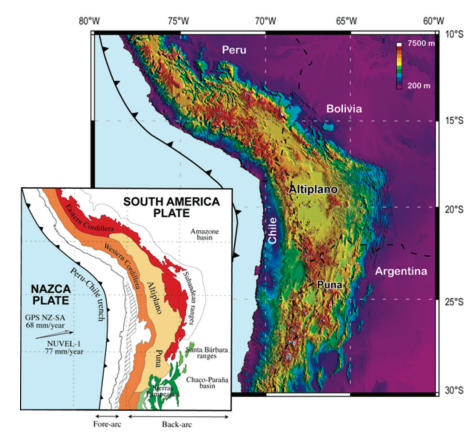
\includegraphics[scale=.6]{./Figures/fig1.png}
	\caption{Fisiografía y unidades geológicas y morfotectónicas de los Andes Centrales\protect\footnotemark.}
	\label{fig:fisiografia}
\end{figure}
\FloatBarrier

La dinámica de los sistemas acuáticos en la Puna argentina está fuertemente influenciada por las fluctuaciones interanuales en las precipitaciones y por eventos climáticos de escala global como El Niño-Oscilación del Sur (ENSO) \cite{trenberth1997definition}. Durante fases cálidas de ENSO, pueden producirse anomalías positivas de precipitación que incrementan temporalmente la superficie cubierta por agua en lagunas y salares. Sin embargo, la magnitud y frecuencia de estos eventos son irregulares y dependen de múltiples factores atmosféricos.

Uno de los principales desafíos para caracterizar estos ambientes radica en la escasez de datos \textit{in situ}. La lejanía geográfica, la falta de infraestructura de monitoreo y las condiciones climáticas adversas dificultan la observación directa y sistemática. La teledetección se usa como una herramienta clave para el estudio de la dinámica hídrica regional, como lo demuestran estudios recientes en regiones altoandinas \cite{saavedra2018changes}.

\footnotetext{Imagen tomada de  \url{https://www.researchgate.net/
publication/342886312}}


El uso de imágenes satelitales multiespectrales y técnicas de teledetección ha cobrado especial relevancia para generar series temporales extensas con datos históricos de sensores como  Landsat \cite{wulder2019landsat}. Esto permite evaluar la evolución de estos cuerpos de agua a lo largo de varias décadas, capturar patrones estacionales, eventos extremos y tendencias de largo plazo. El uso de estas herramientas y técnicas ayuda a mejorar el conocimiento ecológico de los salares y a generar insumos para la toma de decisiones en un contexto de creciente presión sobre los recursos hídricos del altiplano argentino.

%----------------------------------------------------------------------------------------

\section{Contexto del litio en la región}
La región de la Puna argentina se ha convertido en un nodo estratégico dentro del denominado Triángulo del Litio, una zona compartida con Bolivia y Chile que alberga algunas de las mayores reservas de litio del planeta. En esta área, los salares constituyen sistemas hidrogeológicos endorreicos en los que se acumulan salmueras ricas en litio, potasio, boro y otros elementos. Esta riqueza mineral ha dado lugar al despliegue de numerosos proyectos de exploración y explotación minera, particularmente enfocados en el litio en salmuera, una forma no convencional de yacimiento en la que el recurso se encuentra en estado disuelto dentro de acuíferos subterráneos.

Según un relevamiento reciente realizado por López Steinmetz et al. \cite{lopezsteinmetz2024book}, en 2023 existían al menos 90 proyectos de litio tipo salmuera anunciados en el noroeste argentino. Estos proyectos abarcan un amplio espectro de etapas, desde la prospección inicial hasta la operación productiva. Sin embargo, solo el 5,52 \% de la superficie minera otorgada está efectivamente en etapa de producción de litio. A esto se suma un dato llamativo: el 73 \% de las minas concedidas se encuentran fuera de los salares, y el 58\% de los proyectos carecen de datos sobre la concentración de litio en las salmueras, lo que introduce incertidumbres tanto técnicas como ambientales en la gestión de estos recursos.

El sector está dominado por actores privados, quienes controlan el 89\% del total de los 28 752 km² otorgados como concesiones mineras en la región andina argentina. Aun así, la industria mantiene una dinámica competitiva sin alcanzar una completa monopolización: solo tres empresas concentran el 21\% de las concesiones. Esta configuración plantea importantes desafíos para la gobernanza de los recursos, la distribución de beneficios y la gestión ambiental estratégica de los salares.

La regulación y fiscalización de los recursos hídricos en estas zonas cobra entonces una importancia crítica, dado que el proceso extractivo implica la utilización intensiva de agua subterránea, tanto en forma de salmuera como de agua dulce. Si bien representa un porcentaje reducido del uso industrial global, su impacto es significativo en contextos áridos, donde el recurso hídrico es limitado y cumple un rol fundamental para comunidades locales, fauna y ecosistemas.

En este contexto, comprender la distribución espacio-temporal del agua en los salares y su relación con los procesos climáticos se vuelve esencial no solo desde una perspectiva científica, sino también para informar políticas públicas más sostenibles y equitativas.


%----------------------------------------------------------------------------------------

\section{Motivación}

La actividad minera en los salares altoandinos requiere una gran cantidad de agua, utilizada en el bombeo de salmuera y en las operaciones auxiliares de procesamiento. Estudios recientes estiman que la huella hídrica total de un proyecto como Olaroz asciende a 584,1 m\textsuperscript{3} por tonelada de carbonato de litio, con un 92\% correspondiente a salmuera y un 8\% a agua dulce \cite{lopezsteinmetz2024book}.

En paralelo, investigaciones realizadas en el Salar de Atacama y otros sistemas similares muestran que el cambio climático reduce la cobertura nival, eleva la línea de isonieve y disminuye la persistencia estacional de los cuerpos de agua \cite{saavedra2018changes}. Estas transformaciones afectan la recarga natural de los acuíferos y agravan la presión sobre los recursos hídricos superficiales y subterráneos.

Asimismo, estudios limnológicos en lagos salinos del norte de Chile indican que las fluctuaciones térmicas estacionales y la turbidez del agua pueden ser evaluadas mediante sensores remotos como Landsat 8 \cite{delosrios2024lakes}, lo que refuerza la potencialidad de la teledetección para el monitoreo ambiental de salares en zonas remotas.

Frente a este panorama, se plantea la necesidad de contar con herramientas técnicas y replicables que permitan identificar patrones hídricos, anticipar escenarios y orientar decisiones de gestión. La combinación de datos satelitales históricos y técnicas de inteligencia artificial constituye una oportunidad concreta para modelar la ocurrencia de agua en salares y comprender su relación con variables climáticas globales como ENSO.

%----------------------------------------------------------------------------------------

\section{Estado del arte}

En los últimos años, el monitoreo ambiental de ecosistemas altoandinos mediante imágenes satelitales ha ganado relevancia en la comunidad científica. Esto se debe tanto al crecimiento de la minería de litio como a la necesidad de comprender los impactos del cambio climático sobre la disponibilidad de agua en regiones áridas. En este contexto, la combinación de datos de sensores remotos con modelos de aprendizaje automático se presenta como una herramienta robusta para detectar cambios, inferir patrones y generar predicciones sobre sistemas complejos.

Uno de los enfoques más utilizados es el procesamiento multitemporal de imágenes Landsat, que permite evaluar la presencia de cuerpos de agua a partir de índices espectrales como NDWI \textit{(Normalized Difference Water Index)}, NDVI \textit{(Normalized Difference Vegetation Index)} y NDSI \textit{(Normalized Difference Snow Index)}. Estas metodologías han sido aplicadas con éxito en estudios sobre cobertura nival en los Andes \cite{saavedra2018changes} y en la caracterización de lagos salinos mediante parámetros ópticos como turbidez o temperatura superficial \cite{delosrios2024lakes}.

En el ámbito de la minería de litio, el trabajo de López Steinmetz et al. \cite{lopezsteinmetz2024book} destaca la escasa disponibilidad de datos ambientales verificables, especialmente en lo que respecta a la disponibilidad hídrica en salares. Este vacío de información representa una oportunidad para la aplicación de modelos independientes basados en imágenes satelitales.

Por otro lado, existen antecedentes locales relevantes desarrollados en el marco de la Especialización en Inteligencia Artificial de FIUBA. Por ejemplo, Roldán \cite{roldan2023ceia} diseñó un \textit{pipeline} de procesamiento de imágenes aéreas de alta resolución para la clasificación de morfologías de cultivos mediante índices espectrales y redes neuronales convolucionales, en combinación con algoritmos de detección de líneas como la transformada de Hough. Su enfoque sobre datos geoespaciales y procesamiento espectral es comparable con el uso de Landsat en estudios ambientales, aunque aplicado al ámbito agrícola.

Asimismo, Ferrán \cite{ferran2024ceia} integró imágenes Sentinel-2 con datos de sensores terrestres para evaluar la correspondencia entre índices espectrales y observaciones en campo. Su metodología basada en Python y herramientas de código abierto como GeoPandas, Rasterio y OpenEO, puede servir de referencia para la estructuración de \textit{pipelines} multifuente orientados a monitoreo de ecosistemas.

De forma complementaria, Tentor \cite{tentor2023ceiot} desarrolló una plataforma web para la integración y visualización de datos de humedad de suelo, donde se combinan sensores IoT con imágenes satelitales y técnicas de fusión de datos. Su enfoque orientado a toma de decisiones en el ámbito agronómico puede ser extrapolado a problemáticas ambientales como la gestión de recursos hídricos en zonas de extracción minera.

En conjunto, estos antecedentes muestran que existe una base metodológica consolidada para integrar imágenes satelitales, análisis multitemporal e inteligencia artificial en estudios de carácter ambiental y productivo. Sin embargo, aún son escasos los trabajos aplicados específicamente a los salares altoandinos del noroeste argentino, lo que refuerza la pertinencia y originalidad del presente estudio.


%----------------------------------------------------------------------------------------

\section{Objetivos y alcance}

Analizar los patrones temporales de ocurrencia de agua superficial en el Salar de Llullaillaco a partir de imágenes Landsat, e investigar su relación con variables climáticas globales asociadas al fenómeno ENSO mediante técnicas de teledetección, análisis de series temporales.

Dentro de los objetivos específicos, se pueden mencionar los siguientes:

\begin{itemize}
    \item Generar series temporales de índices espectrales (NDWI) a partir de imágenes Landsat 5, 7 y 8 para identificar zonas con presencia estacional o persistente de agua superficial.
    \item Preprocesar y normalizar variables climáticas relevantes (Niño 3.4, SOI, MEI) para su análisis conjunto con los datos satelitales.
    \item Integrar y correlacionar los índices espectrales con series mensuales de indicadores climáticos globales (Niño 3.4, SOI, MEI) para evaluar relaciones potenciales.
    \item Aplicar modelos de análisis de series temporales (SARIMA y VAR) y pruebas de causalidad de Granger para identificar dependencias y relaciones dinámicas entre las variables.
    \item Entrenar y evaluar modelos de aprendizaje automático para generar predicciones exploratorias sobre la ocurrencia de agua superficial.
    \item Visualizar y analizar temporalmente los resultados mediante gráficos interpretativos y funciones de respuesta al impulso (IRF).
\end{itemize}

El alcance del trabajo se enfoca exclusivamente en el análisis del Salar de Llullaillaco, ubicado en la región de la Puna argentina. Se utilizaron imágenes ópticas Landsat procesadas en la plataforma Google Earth Engine. El estudio se limita a la detección de agua superficial mediante índices espectrales (NDWI), sin abordar el modelado de agua subterránea. Asimismo, se emplean únicamente variables climáticas globales con resolución mensual asociadas a ENSO (Niño 3.4, SOI, MEI), sin incorporar datos meteorológicos locales.

No se contempla la validación directa en campo, aunque se prevé la comparación con antecedentes bibliográficos y series públicas disponibles para la región. Los modelos predictivos utilizados tendrán un carácter exploratorio, orientado a generar una base metodológica replicable que permita evaluar dinámicas hidrológicas en ecosistemas salinos vulnerables sometidos a presión climática y extractiva.


%----------------------------------------------------------------------------------------

\chapter{Introducción específica} % Main chapter title

\label{Chapter2}

%----------------------------------------------------------------------------------------
%	SECTION 1
%----------------------------------------------------------------------------------------
En este capítulo se presenta una introducción técnica a la temática abordada en el trabajo. 

\section{Requerimientos}
\label{sec:ejemplo}
A continuación, se detallan los principales requerimientos funcionales y técnicos.

\subsection*{Requerimientos funcionales}

\begin{itemize}
\item Obtener series temporales de cobertura de agua superficial en el Salar de Llullaillaco, a partir de índices espectrales derivados de imágenes Landsat.
\item Correlacionar los patrones de presencia de agua con variables climáticas globales asociadas al ENSO (Niño 3.4, SOI, MEI).
\item Generar modelos predictivos de ocurrencia de agua mediante el uso algoritmos de aprendizaje supervisado.
\item Visualizar los resultados mediante mapas y gráficos temporales que permitan interpretar los patrones hidrológicos en relación con el clima.
\end{itemize}

\subsection*{Requerimientos técnicos}

\begin{itemize}
\item Acceso a la plataforma Google Earth Engine (GEE) para el procesamiento de imágenes satelitales Landsat 5, 7 y 8.
\item Dataset mensual de los índices climáticos de ENSO: Niño 3.4, \textit{Southern Oscillation Index (SOI)}, y \textit{Multivariate ENSO Index (MEI)}.
\item Computadora con entorno de desarrollo Python, con acceso a bibliotecas como PANDAS, NUMPY, MATPLOTLIB, SKLEARN, TORCH.
\item Conexión a INTERNET para descarga de datos y acceso a \textit{notebooks} en la nube.
\end{itemize}



%----------------------------------------------------------------------------------------
%	SECTION 2
%----------------------------------------------------------------------------------------

\section{Técnicas utilizadas}

El desarrollo de este trabajo se basa en la combinación de técnicas de teledetección, análisis multitemporal y aprendizaje automático, integradas en un flujo de trabajo que permite monitorear la presencia de agua superficial en el Salar de Llullaillaco y explorar su relación con la variabilidad climática regional.

\subsection*{Google Earth Engine (GEE)}

Se utilizó la plataforma GEE para el acceso y procesamiento de imágenes Landsat 5, 7 y 8, con el mismo enfoque usado por \cite{ferran2024ceia, roldan2023ceia}. GEE permite aplicar filtros temporales, máscaras de nubes, recortes espaciales y cálculos de índices espectrales sobre áreas definidas, con eficiencia y escalabilidad.


\subsection*{Sobre los índices espectrales}

El índice espectral utilizado en este trabajo fue el NDWI (\textit{Normalized Difference Water Index}). Este índice se basa en relaciones matemáticas entre bandas del espectro electromagnético que capturan variaciones en la reflectancia del terreno. Estas métricas se fundamentan en estudios de respuesta espectral diferencial de distintos tipos de cobertura superficial, como agua, vegetación o nieve, especialmente visibles en las bandas verde, roja, infrarroja cercana (NIR) y de onda corta (SWIR).

Tal como se observa en trabajos clásicos de teledetección \cite{tucker1979red, huete1988soil}, la vegetación sana refleja fuertemente en el infrarrojo cercano y absorbe en la banda roja, mientras que el agua y la nieve presentan perfiles espectrales contrastantes. Estas propiedades permiten construir índices que destacan las coberturas de interés.


En este trabajo se usó principalmente NDWI como un marco conceptual útil para entender las diferencias espectrales de las cubiertas superficiales analizadas en el Salar de Llullaillaco.


\subsection*{Índices espectrales utilizados}

Los índices seleccionados permiten caracterizar el comportamiento espectral del suelo y del agua en ambientes de alta reflectancia como los salares:
A continuación se presentan los índices espectrales utilizados para la detección y clasificación de coberturas en imágenes satelitales:

\begin{itemize}
    \item NDWI: resalta la presencia de agua superficial ya que emplea las bandas del verde y el infrarrojo cercano (NIR). Su expresión matemática se observa en la ecuación \ref{eq:ndwi}:

    \begin{equation}
        \label{eq:ndwi}
        NDWI = \frac{\text{Green} - \text{NIR}}{\text{Green} + \text{NIR}}
    \end{equation}

\end{itemize}


\begin{figure}[htpb]
	\centering
	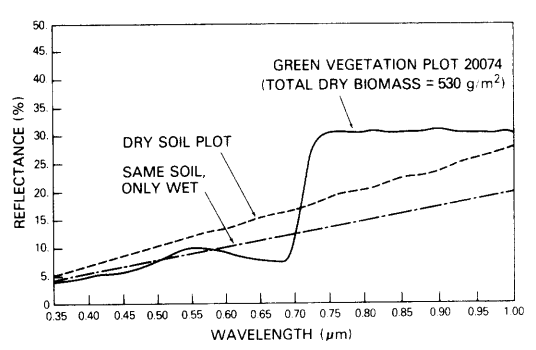
\includegraphics[scale=.5]{Figures/fig3.png}
	\caption{Reflectancias espectrales de suelo seco, suelo húmedo y vegetación completamente verde\protect\footnotemark.}
	\label{fig:palabraIngles}
\end{figure}

\footnotetext{Imagen tomada de \cite{tucker1979red}.}}


\subsection*{Imágenes Landsat utilizadas}

Para este trabajo se emplearon imágenes ópticas de las misiones \Landsat 5 TM, Landsat 7 ETM+ y Landsat 8 OLI, disponibles en la plataforma GEE como colecciones. Las colecciones empleadas de Google Earth Engine fueron:

\begin{itemize}
    \item \texttt{LANDSAT/LT05/C02/T1\_L2} — Landsat 5 TM, colección nivel 2 (surface reflectance).
    \item \texttt{LANDSAT/LE07/C02/T1\_L2} — Landsat 7 ETM+, colección nivel 2.
    \item \texttt{LANDSAT/LC08/C02/T1\_L2} — Landsat 8 OLI, colección nivel 2.
\end{itemize}

Estas imágenes corresponden a productos de nivel 2, que incluyen correcciones atmosféricas (Surface Reflectance) y enmascaramiento de nubes mediante algoritmos QA/QC. Se seleccionaron todas las escenas disponibles y se priorizaron aquellas sin nubes y con cobertura adecuada del Salar de Llullaillaco.

Las bandas empleadas en los cálculos de índices espectrales fueron:

\begin{itemize}
    \item Landsat 5 TM:
    \begin{itemize}
        \item Green: Band 2 (0,52–0,60 µm)
        \item Red: Band 3 (0,63–0,69 µm)
        \item NIR: Band 4 (0,76–0,90 µm)
        \item SWIR1: Band 5 (1,55–1,75 µm)
    \end{itemize}
    
    \item Landsat 7 ETM+:
    \begin{itemize}
        \item Green: Band 2 (0,52–0,60 µm)
        \item Red: Band 3 (0,63–0,69 µm)
        \item NIR: Band 4 (0,77–0,90 µm)
        \item SWIR1: Band 5 (1,55–1,75 µm)
    \end{itemize}

    \item Landsat 8 OLI:
    \begin{itemize}
        \item Green: Band 3 (0,53–0,59 µm)
        \item Red: Band 4 (0,64–0,67 µm)
        \item NIR: Band 5 (0,85–0,88 µm)
        \item SWIR1: Band 6 (1,57–1,65 µm)
    \end{itemize}
\end{itemize}


Estas bandas fueron utilizadas para calcular el ìndice NDWI. Se ajustaron las combinaciones de las mismas según el sensor. La consistencia intersensorial fue manejada a través de normalización espectral mensual y máscaras de calidad provistas por GEE.

\subsection*{Variables climáticas ENSO}

El fenómeno El Niño-Oscilación del Sur (ENSO) es uno de los principales moduladores del clima a escala interanual, y tiene un impacto significativo en los regímenes de precipitación y temperatura en América del Sur. ENSO es un sistema acoplado océano-atmósfera que alterna entre tres fases:

\begin{itemize}
    \item {El Niño: fase cálida, asociada a un aumento de la temperatura superficial del mar (SST) en el Pacífico ecuatorial central y oriental.
    \item La Niña: fase fría, caracterizada por anomalías negativas de SST en la misma región.
    \item Neutral: ausencia de anomalías significativas en las condiciones oceánicas y atmosféricas.
\end{itemize}

Estas variaciones alteran la circulación atmosférica a nivel planetario, por ejemplo la intensidad de los vientos alisios, el transporte de humedad, y la posición de la Zona de Convergencia Intertropical (ZCIT). En regiones como la Puna argentina, se ha documentado que las fases de ENSO afectan directamente los patrones de precipitación y, por ende, la disponibilidad de agua superficial y la recarga de los salares.

Para capturar cuantitativamente la influencia de ENSO, en este trabajo se utilizaron tres índices climáticos de carácter mensual:

\begin{itemize}
    \item Niño 3.4 Index (ONI): representa la anomalía mensual de la temperatura superficial del mar en la región 5°N–5°S, 170°W–120°W. Es la métrica más común para definir la fase cálida (El Niño) o fría (La Niña) de ENSO \cite{nino34index}.

    \item Southern Oscillation Index (SOI): calculado a partir de la diferencia de presión atmosférica entre Tahití y Darwin. Un valor negativo indica condiciones de El Niño, mientras que uno positivo sugiere La Niña \cite{soiindex}.

    \item Multivariate ENSO Index (MEI.v2): combina variables atmosféricas y oceánicas (SST, presión, viento zonal y meridional, etc.) en un índice multivariado más robusto \cite{meiindex}.
\end{itemize}

Estos indicadores se obtuvieron de fuentes oficiales como la \textit{NOAA Climate Prediction Center} y el \textit{Physical Sciences Laboratory} de EE.UU. y fueron alineados mensualmente con las series de datos espectrales obtenidas de imágenes Landsat, en el período 2000–2024.

Incluir estos índices como variables explicativas permite explorar la posible relación entre eventos ENSO y la presencia de agua superficial en el Salar de Llullaillaco, se aporta una perspectiva climática regional al análisis hidrológico local.

%----------------------------------------------------------------------------------------
%	SECTION 3
%----------------------------------------------------------------------------------------

\section{Herramientas y bibliotecas utilizadas}


\subsection*{Entornos de trabajo}

\begin{itemize}
    \item Google Earth Engine (GEE): utilizada para acceder, filtrar y procesar imágenes Landsat. 
    
    \item Google Colab: facilita la integración con GEE mediante exportación de datos, así como la implementación de modelos de \textit{machine learning} sin necesidad de recursos locales avanzados.

    \item Python 3.10: lenguaje principal utilizado para análisis de datos, entrenamiento de modelos, generación de gráficos y administración de \textit{workflows}.
\end{itemize}


\subsection*{Bibliotecas y frameworks}

Las siguientes bibliotecas fueron utilizadas en distintas etapas del flujo de trabajo:

\begin{itemize}
    \item \texttt{PANDAS}: manipulación de estructuras tabulares y series temporales. Versión 1.5.3.
    \item \texttt{NUMPY}: operaciones numéricas vectorizadas y manejo eficiente de arreglos multidimensionales. Versión 1.24.3.
    \item \texttt{MATPLOTLIB} y \texttt{SEABORN}: generación de gráficos, visualización de tendencias temporales y resultados de modelos. Versiones 3.6.2 y 0.12.2 respectivamente.
    \item \texttt{SCIKIT-LEARN}: implementación de modelos Random Forest, validación cruzada, métricas de clasificación y selección de variables. Versión 1.1.3.
    \item \texttt{PYTORCH}: entrenamiento de redes neuronales profundas, arquitectura multicapa y optimización basada en descenso de gradiente. Versión 2.0.1.
    \item \texttt{PYTHON}: lenguaje principal utilizado para análisis de datos, entrenamiento de modelos, generación de gráficos y administración de workflows. Versión 3.10.
    \item \texttt{Google Eart Engine}: plataforma web de procesamiento satelital utilizada para acceder, filtrar y procesar imágenes Landsat, y calcular índices espectrales. API JS (Web) y API Python versión 0.1.365.
    \item \texttt{Google Colab}: entorno de ejecución en la nube usado para integración con GEE y entrenamiento de modelos. Versión utilizada: mayo 2025.
\end{itemize}



Además, se utilizaron funciones propias escritas en Python para carga de datos, limpieza, ingeniería de variables y evaluación de modelos.



%----------------------------------------------------------------------------------------
\chapter{Diseño e implementación} % Main chapter title

\label{Chapter3} % Change X to a consecutive number; for referencing this chapter elsewhere, use \ref{ChapterX}

Este capítulo presenta la solución desarrollada para abordar el análisis multitemporal de la ocurrencia de agua en el Salar de Llullaillaco. Se describen la arquitectura general del sistema, el preprocesamiento aplicado a las imágenes satelitales, el tratamiento de datos climáticos y espectrales, el análisis temporal y la correlación con los indicadores del fenómeno ENSO. 


\definecolor{mygreen}{rgb}{0,0.6,0}
\definecolor{mygray}{rgb}{0.5,0.5,0.5}
\definecolor{mymauve}{rgb}{0.58,0,0.82}

%%%%%%%%%%%%%%%%%%%%%%%%%%%%%%%%%%%%%%%%%%%%%%%%%%%%%%%%%%%%%%%%%%%%%%%%%%%%%
% parámetros para configurar el formato del código en los entornos lstlisting
%%%%%%%%%%%%%%%%%%%%%%%%%%%%%%%%%%%%%%%%%%%%%%%%%%%%%%%%%%%%%%%%%%%%%%%%%%%%%
\lstset{ %
  backgroundcolor=\color{white},   % choose the background color; you must add \usepackage{color} or \usepackage{xcolor}
  basicstyle=\footnotesize,        % the size of the fonts that are used for the code
  breakatwhitespace=false,         % sets if automatic breaks should only happen at whitespace
  breaklines=true,                 % sets automatic line breaking
  captionpos=b,                    % sets the caption-position to bottom
  commentstyle=\color{mygreen},    % comment style
  deletekeywords={...},            % if you want to delete keywords from the given language
  %escapeinside={\%*}{*)},          % if you want to add LaTeX within your code
  %extendedchars=true,              % lets you use non-ASCII characters; for 8-bits encodings only, does not work with UTF-8
  %frame=single,	                % adds a frame around the code
  keepspaces=true,                 % keeps spaces in text, useful for keeping indentation of code (possibly needs columns=flexible)
  keywordstyle=\color{blue},       % keyword style
  language=[ANSI]C,                % the language of the code
  %otherkeywords={*,...},           % if you want to add more keywords to the set
  numbers=left,                    % where to put the line-numbers; possible values are (none, left, right)
  numbersep=5pt,                   % how far the line-numbers are from the code
  numberstyle=\tiny\color{mygray}, % the style that is used for the line-numbers
  rulecolor=\color{black},         % if not set, the frame-color may be changed on line-breaks within not-black text (e.g. comments (green here))
  showspaces=false,                % show spaces everywhere adding particular underscores; it overrides 'showstringspaces'
  showstringspaces=false,          % underline spaces within strings only
  showtabs=false,                  % show tabs within strings adding particular underscores
  stepnumber=1,                    % the step between two line-numbers. If it's 1, each line will be numbered
  stringstyle=\color{mymauve},     % string literal style
  tabsize=2,	                   % sets default tabsize to 2 spaces
  title=\lstname,                  % show the filename of files included with \lstinputlisting; also try caption instead of title
  morecomment=[s]{/*}{*/}
}


%----------------------------------------------------------------------------------------
%	SECTION 1
%----------------------------------------------------------------------------------------

\section{Área de estudio y representación espacial}

La cuenca hidrográfica del  Salar de Llullaillaco incluye sectores volcánicos elevados y drenajes que desembocan sobre el salar lo que genera condiciones potenciales para la ocurrencia de cuerpos de agua temporales. Esta delimitación hidrológica se muestra en la figura~\ref{fig:cuenca_llullaillaco}.


\begin{figure}[htpb]
	\centering
	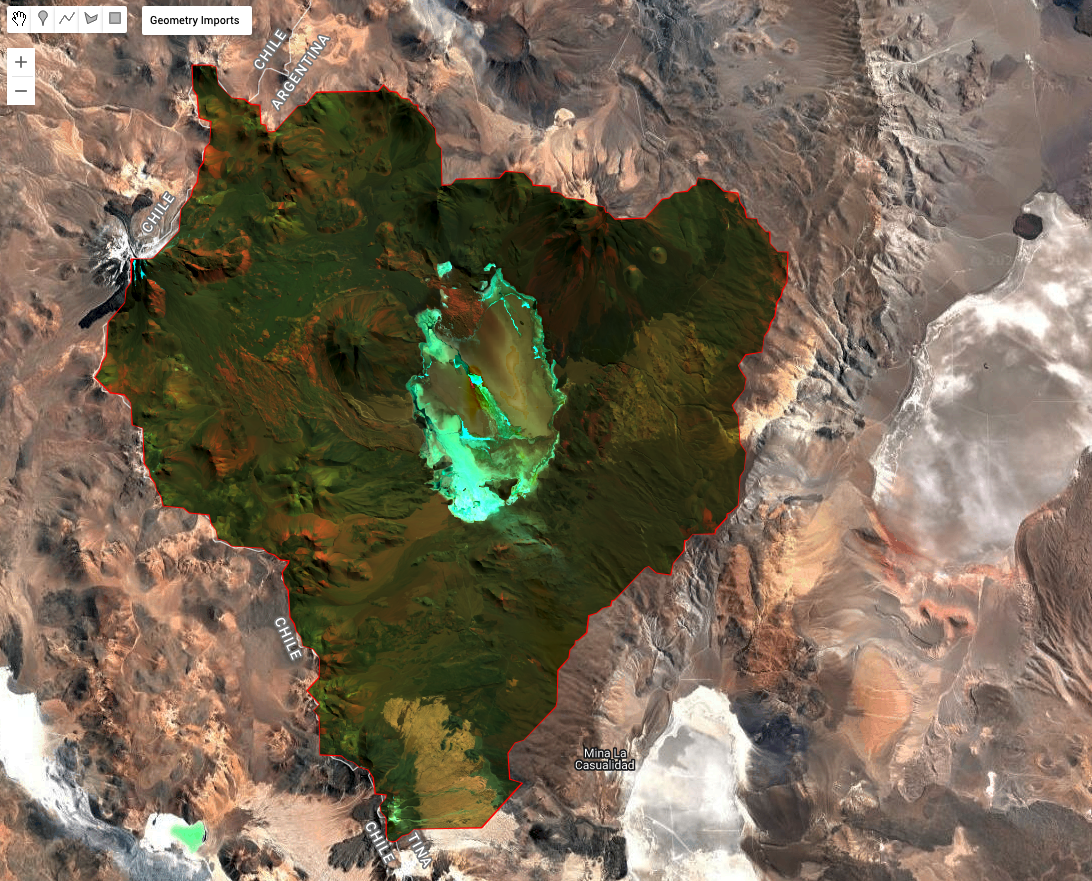
\includegraphics[scale=.3]{Figures/fig5.png}
	\caption{Cuenca del Salar de Llullaillaco.}
	\label{fig:cuenca_llullaillaco}
\end{figure}

Para determinar las zonas con mayor recurrencia de agua superficial, se implementó un procedimiento de clasificación píxel a píxel basado en la aplicación de un umbral de NDWI $>0{,}2$ sobre cada imagen mensual. Este proceso permitió generar una máscara binaria de agua para cada imagen que se integró posteriormente en un mapa de calor de ocurrencia. La proporción de imágenes en las que un píxel fue clasificado como \texttt{agua} se interpreta como una probabilidad relativa de presencia hídrica.

El resultado de este análisis se presenta en la figura~\ref{fig:mapa_ocurrencias}, donde se observan claramente las zonas de mayor persistencia de agua dentro del salar.


\begin{figure}[htpb]
	\centering
	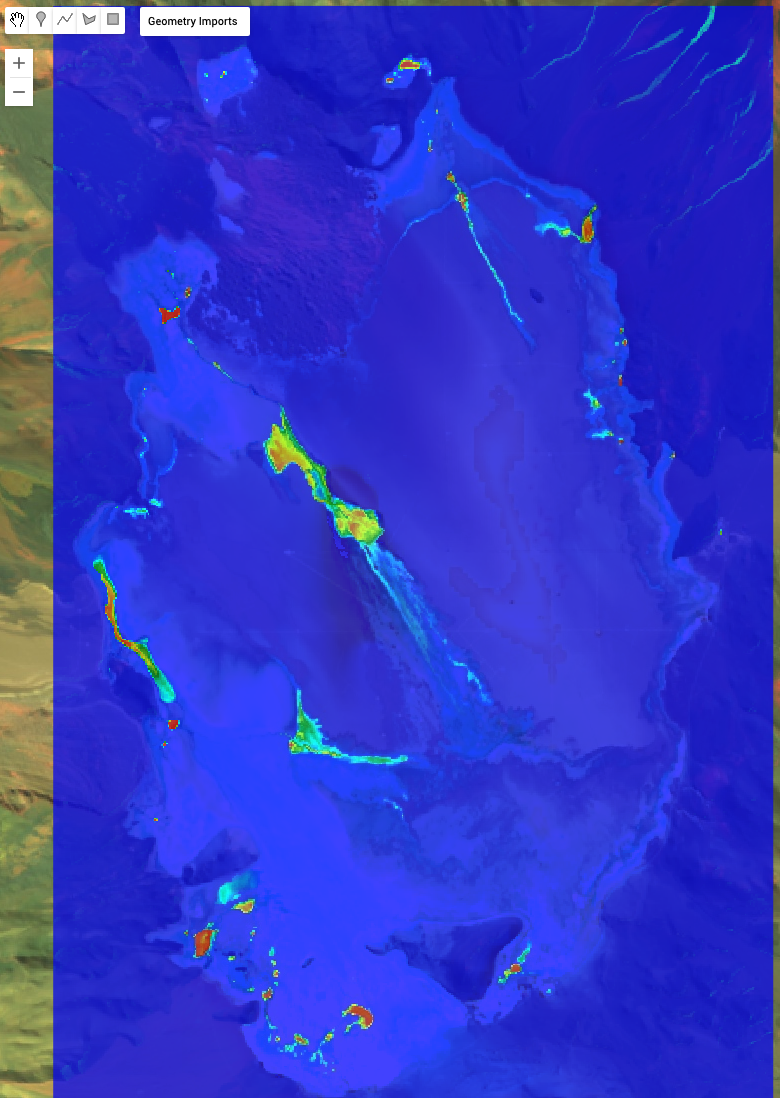
\includegraphics[scale=.3]{Figures/fig6.png}
	\caption{Mapa de calor de ocurrencia de agua superficial en el Salar de Llullaillaco. Colores más cálidos indican mayor frecuencia.}
	\label{fig:mapa_ocurrencias}
\end{figure}



\subsubsection*{Recorte geográfico y generación de mosaicos}

La zona de estudio fue definida a partir de un polígono de delimitación del Salar de Llullaillaco, construido con herramientas SIG y validado mediante visualización satelital. A cada imagen Landsat filtrada se le aplicó un recorte espacial que limita el análisis exclusivamente a esta región.

Dado que cada misión Landsat posee distinto patrón de cobertura espacial y que algunas escenas individuales no cubren completamente el salar, se generaron mosaicos mensuales por misión donde se usó la mediana de los valores de reflectancia en cada píxel. Este procedimiento homogeniza la observación mensual y permite una mejor comparación interanual.


Se observa que la zona con mayor recurrencia de agua corresponde a la laguna central del salar, un cuerpo de agua de morfología alargada, ubicado en el eje norte-sur de la depresión principal. Por este motivo, el análisis estadístico y la posterior implementación de modelos predictivos se enfocan principalmente en esa área. Desde el punto de vista de la biodiversidad esta laguna es la que presenta mayor concentración de fauna acuática.

La figura~\ref{fig:epoca_seca_hum}  permiten visualizar el cambio estacional en la extensión de la laguna central del Salar de Llullaillaco y muestran diferencias notables entre los meses secos y húmedos.


\begin{figure}[ht]
        \centering
        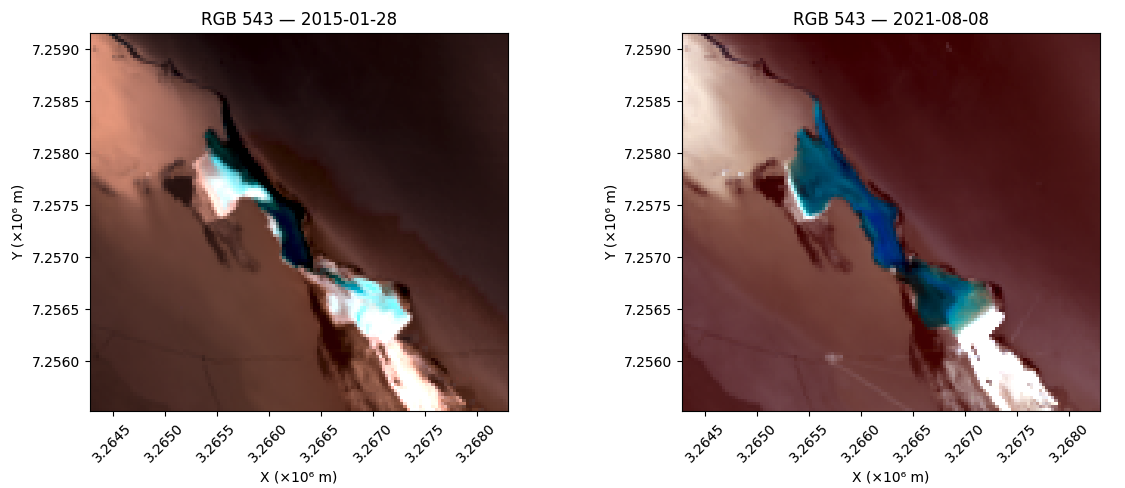
\includegraphics[scale=.37]
        {Figures/rbg_cap3_a.png}
        \caption{Imagen en composición RGB 543. Izquierda: época seca (enero 2015). Derecha: época húmeda (agosto 2021).}
        \label{fig:epoca_seca_hum}
\end{figure}


La figura~\ref{fig:ndwi_seco_hum} muestra el índice NDWI para dos fechas representativas. Valores positivos de NDWI indican presencia de agua.


\begin{figure}[ht]
        \centering
        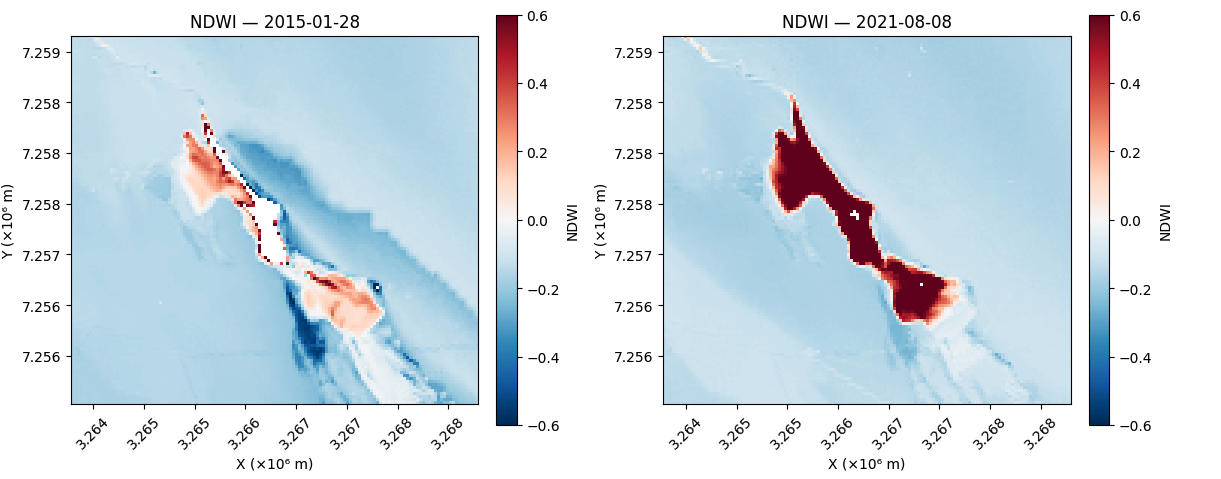
\includegraphics[scale=.37]
        {Figures/rgb_cap3_b.png}
        \caption{Indice NDWI. Izquierda: época seca (enero 2015). Derecha: época húmeda (agosto 2021).}
        \label{fig:ndwi_seco_hum}
\end{figure}


\newpage
\section{Arquitectura general del sistema}

El sistema propuesto se basa en una arquitectura modular que integra tecnologías de teledetección, análisis de datos climáticos y modelado basado en inteligencia artificial. Esta integración permite automatizar el proceso de detección de agua superficial en el Salar de Llullaillaco y explorar su posible relación con variables climáticas globales como las asociadas al fenómeno ENSO.

\subsection*{Componentes principales}

La arquitectura general del sistema se compone de tres bloques funcionales principales (ver figura \ref{fig:arquitectura_general}):

\begin{enumerate}
    \item Bloque de adquisición y preprocesamiento: se encarga de la descarga, filtrado y procesamiento de imágenes satelitales Landsat desde la plataforma GEE. En esta etapa se recorta el área de interés, se eliminan imágenes con cobertura nubosa o mala calidad y se calcula el índices espectral NDWI.
    
    \item Bloque de integración climática: incorpora las series mensuales de los indicadores climáticos ENSO (Niño 3.4, SOI y MEI), obtenidas de fuentes oficiales (NOAA, BOM, PSL), alineadas temporalmente con las imágenes satelitales para permitir su análisis conjunto.

    \item Bloque de análisis y modelado: el análisis incluyó pruebas de estacionariedad (ADF, KPSS, PP), funciones de autocorrelación (ACF, PACF) y la aplicación de modelos SARIMA y VAR, evaluando su capacidad predictiva mediante métricas de error (MSE, RMSE, MAE). Se usaron datos exportados desde GEE y combinados con variables climáticas. La implementación y validación se realizó en Google Colab con Python. De esta manera, se obtuvo replicabilidad, visualización y análisis estadístico de los resultados.
\end{enumerate}

\begin{figure}[htpb]
	\centering
	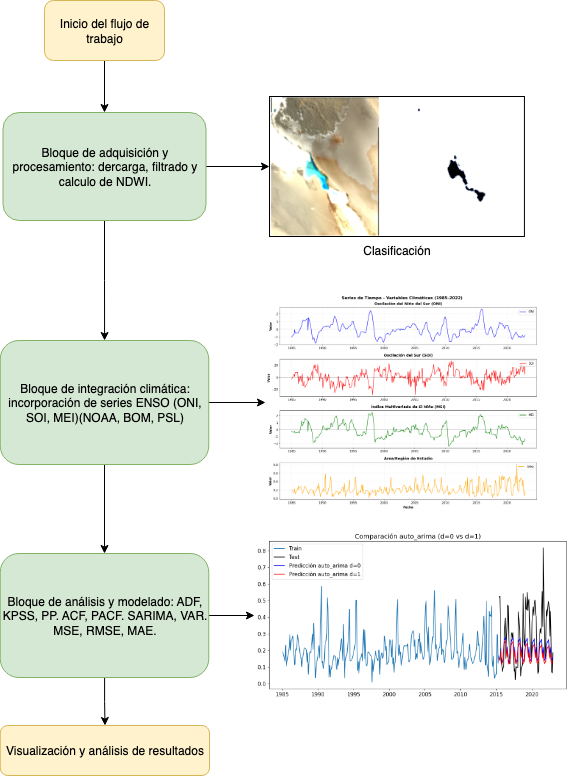
\includegraphics[scale=.6]{Figures/Arqui_TTFB.png}
	\caption{Arquitectura general del sistema: desde la adquisición hasta el modelado.}
	\label{fig:arquitectura_general}
\end{figure}


\subsection*{Flujo de trabajo detallado}

El flujo de trabajo completo incluye las siguientes etapas:

\begin{enumerate}
    \item Extracción satelital: se utilizaron las colecciones Landsat 5, Landsat 7 y Landsat 8 en GEE. Se seleccionaron imágenes con menos del 20\% de nubosidad y se recortaron al polígono del salar.

    \item Cálculo de índices: se calcularon mensualmente los valores medios de NDWI. Se generaron gráficos mensuales y una serie temporal multianual.

    \item Exportación de datos: los datos procesados en GEE fueron exportados en formato CSV y GeoTIFF para su análisis en Python.

    \item Integración con ENSO: se descargaron los valores de Niño 3.4, SOI y MEI, y se alinearon con las fechas de cada imagen mensual. Se realizaron pruebas de normalización y detección de valores atípicos.

    \item Modelado predictivo: se entrenaron modelos exploratorios para predecir la presencia/ausencia de agua en función de los índices espectrales y climáticos. Se utilizaron validaciones cruzadas y análisis de correlaciones.

    \item Visualización de resultados: se generaron mapas de ocurrencia de agua, gráficos de correlación y visualizaciones de precisión de modelos, con el objetivo de interpretar los patrones históricos y su variabilidad.
\end{enumerate}


\subsection*{Ventajas de la arquitectura}

Esta arquitectura ofrece múltiples beneficios:

\begin{itemize}
    \item Permite reproducibilidad total del flujo de trabajo mediante scripts abiertos en GEE y notebooks Python en Colab.
    \item Es escalable a otros salares o humedales de altura, con la modificación del polígono de entrada y el rango de fechas.
    \item Facilita la incorporación de nuevas fuentes climáticas o nuevos sensores remotos sin rediseñar el sistema.
    \item Optimiza el uso de recursos mediante plataformas en la nube, sin requerimientos de hardware local.
\end{itemize}

Esta solución integrada proporciona una herramienta robusta para el análisis ambiental en zonas remotas como la Puna. Su estructura modular, su compatibilidad con datos abiertos y su orientación hacia el análisis multitemporal y predictivo la convierten en una alternativa metodológica replicable en estudios de monitoreo hídrico, cambio climático y gestión territorial.


\section{Preprocesamiento de imágenes}

El preprocesamiento de imágenes satelitales constituye una etapa crítica en todo análisis multitemporal con sensores remotos. En este estudio, se utilizaron imágenes ópticas provenientes de las misiones Landsat 5 TM, Landsat 7 ETM+ y Landsat 8 OLI, accedidas desde la plataforma Google Earth Engine, que permite el procesamiento en la nube con acceso a colecciones históricas de datos corregidos radiométrica y atmosféricamente.

El objetivo del preprocesamiento fue generar series temporales limpias y comparables en el tiempo, con el fin de maximizar la calidad de los datos utilizados que son fundamentales para la detección de cuerpos de agua y vegetación residual. 

\subsubsection*{Selección y filtrado de imágenes}

Las colecciones seleccionadas corresponden a los productos nivel 2 (\texttt{L2}), que contienen valores de reflectancia de superficie corregidos atmosféricamente. Los identificadores de las colecciones utilizadas fueron:

\begin{itemize}
    \item \texttt{LANDSAT/LT05/C02/T1\_L2} para Landsat 5.
    \item \texttt{LANDSAT/LE07/C02/T1\_L2} para Landsat 7.
    \item \texttt{LANDSAT/LC08/C02/T1\_L2} para Landsat 8.
\end{itemize}

El filtrado incluyó:
\begin{itemize}
    \item Eliminación de imágenes con cobertura nubosa mayor al 20\% en la región de interés.
    \item Aplicación de máscaras QA (\textit{Quality Assessment}) para excluir píxeles cubiertos por nubes, sombras y nieve.
    \item Restricción temporal entre 1990 y 2023 y priorización de los meses húmedos (enero–abril) para asegurar observaciones relevantes.
\end{itemize}

Este filtrado permitió construir una base de imágenes consistente y sin anomalías atmosféricas notorias, adecuada para los siguientes pasos del análisis.



\subsubsection*{Corrección espectral intersensor}

Debido a diferencias en las respuestas espectrales entre las misiones (especialmente entre TM/ETM+ y OLI), se aplicó una normalización espectral basada en técnicas de remapeo lineal, tal como se propone en la literatura para combinar series temporales Landsat \parencite{roy2016characterization, roy2014landsat8}. Esto garantiza que las diferencias observadas en el índice NDWI no respondan a variaciones instrumentales sino a cambios reales en superficie.

\subsubsection*{Cálculo de índices espectrales}

Una vez preprocesadas las imágenes, se calcularon los índices espectrales mensuales para cada misión mediante el uso de las bandas adecuadas. Las bandas utilizadas para cada misión se explicaron en el capitulo anterior.

Los valores resultantes fueron exportados como series mensuales promedio para todo el salar, así como también como mapas raster por mes. Esto permitió visualizar la evolución temporal y espacial de la ocurrencia de agua superficial.

\section{Tratamiento de datos }

Esta sección presenta el tratamiento realizado sobre los datos satelitales y climáticos utilizados en el proyecto. Se detallan los criterios de selección, filtrado y preprocesamiento aplicados en la plataforma GEE, así como la integración posterior de variables climáticas globales.

\subsection*{Imágenes satelitales y período de análisis}

Se utilizaron imágenes de las misiones Landsat 5 TM, Landsat 7 ETM+ y Landsat 8 OLI, todas en su versión de corrección atmosférica de superficie (Level 2) disponible en GEE.

Para la construcción de la serie temporal se consultó las colecciones en la plataforma Google Earth Engine, correspondiente a productos de nivel 2 de Landsat 8. La selección de imágenes se restringió al polígono del Salar de Llullaillaco, al período comprendido entre 2015 y 2022, y a escenas con una cobertura nubosa menor al 20\%. Adicionalmente, se aplicó un enmascaramiento de calidad para remover nubes y sombras, con el fin de asegurar que los valores espectrales utilizados reflejaran las condiciones reales de superficie.


Si bien la misión Landsat 7 ETM+ estuvo operativa entre 1999 y 2021, su uso en este proyecto fue limitado debido a restricciones de calidad impuestas por el \textit{Scan Line Corrector (SLC)}. Este componente falló en mayo de 2003 desde donde se generaron pérdidas sistemáticas de cobertura espacial en las imágenes posteriores. Aunque en GEE existen funciones para rellenar o enmascarar los bordes afectados, se priorizó evitar la inclusión de imágenes con geometría incompleta o necesidad de interpolación espacial forzada.

La misión Landsat 5 TM fue seleccionada como fuente principal de imágenes anteriores al año 2011, ya que proporcionó datos continuos entre los años 2000 y 2011 sin fallas estructurales. Su cobertura en la región fue consistente durante la ventana húmeda seleccionada (enero a abril), con una densidad de imágenes suficiente para construir una serie temporal representativa.

Por otro lado, Landsat 8 OLI fue utilizado como principal fuente para el período comprendido entre los años 2013 y 2024. 

En la figura ~\ref{fig:cob_temporal} y en la tabla ~\ref{tab:periodos_landsat} se muestran los períodos de tiempo usados. Es necesario mencionar que debido a la superposición entre Landsat 5 TM y Landsat 7 ETM+ se decidió trabajar solo con Landsat 5 TM y Landsat 8 OLI. Se generó una brecha sin imágenes de 12 meses entre febrero de 2012 y febrero de 2013.

\begin{figure}[ht]
        \centering
        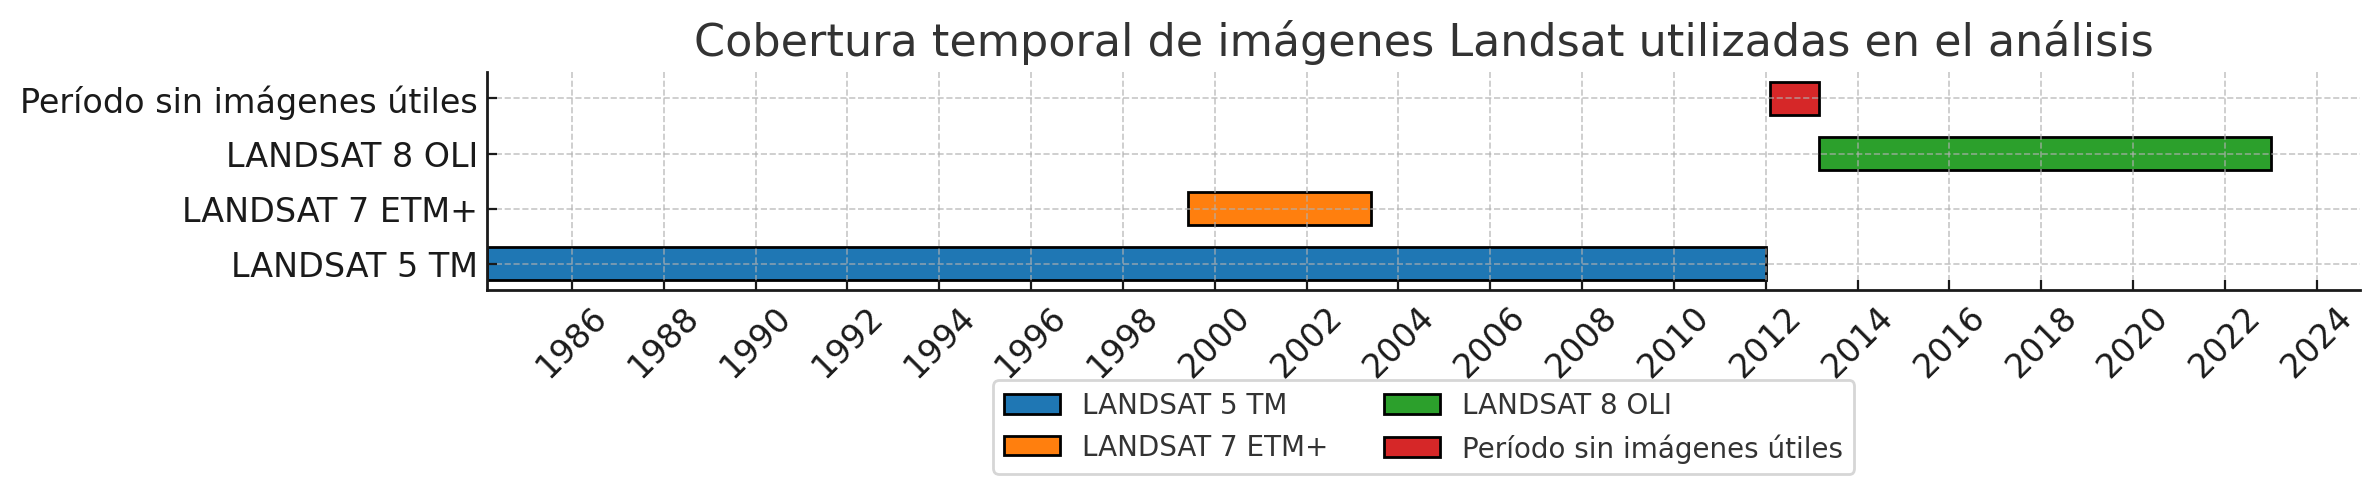
\includegraphics[scale=.4]
        {Figures/fig11.png}
        \caption{Cobertura temporal de las imágenes usadas.}
        \label{fig:cob_temporal}
\end{figure}

En resumen, la elección de misiones respondió a un compromiso entre calidad geométrica, continuidad temporal y cobertura atmosférica. Además,  se priorizó la robustez de las series en períodos relevantes para el análisis hidrológico del salar. En la figura ~\ref{fig:cant_imagenes} y en la tabla ~\ref{tab:periodos_landsat} se muestra la cantidad de imagenes usadas. 


\begin{table}[h]
	\centering
	\caption[Períodos Landsat]{Períodos de utilización de imágenes satelitales por misión Landsat en el presente estudio.}
	\begin{tabular}{l c c c}    
		\toprule
		\textbf{Misión}     & \textbf{Inicio (mes/año)} & \textbf{Fin (mes/año)} & \textbf{Cantidad de imágenes} \\
		\midrule
		Landsat 5 TM        & Marzo 1984   & Enero 2012        & 338 \\		
		Landsat 7 ETM+      & Junio 1999   & Mayo 2003         & no empleadas \\
		Landsat 8 OLI       & Marzo 2013   & Diciembre 2022    & 209 \\
		\bottomrule
	\end{tabular}
        \hline
	\label{tab:periodos_landsat}
\end{table}

\begin{figure}[ht]
        \centering
        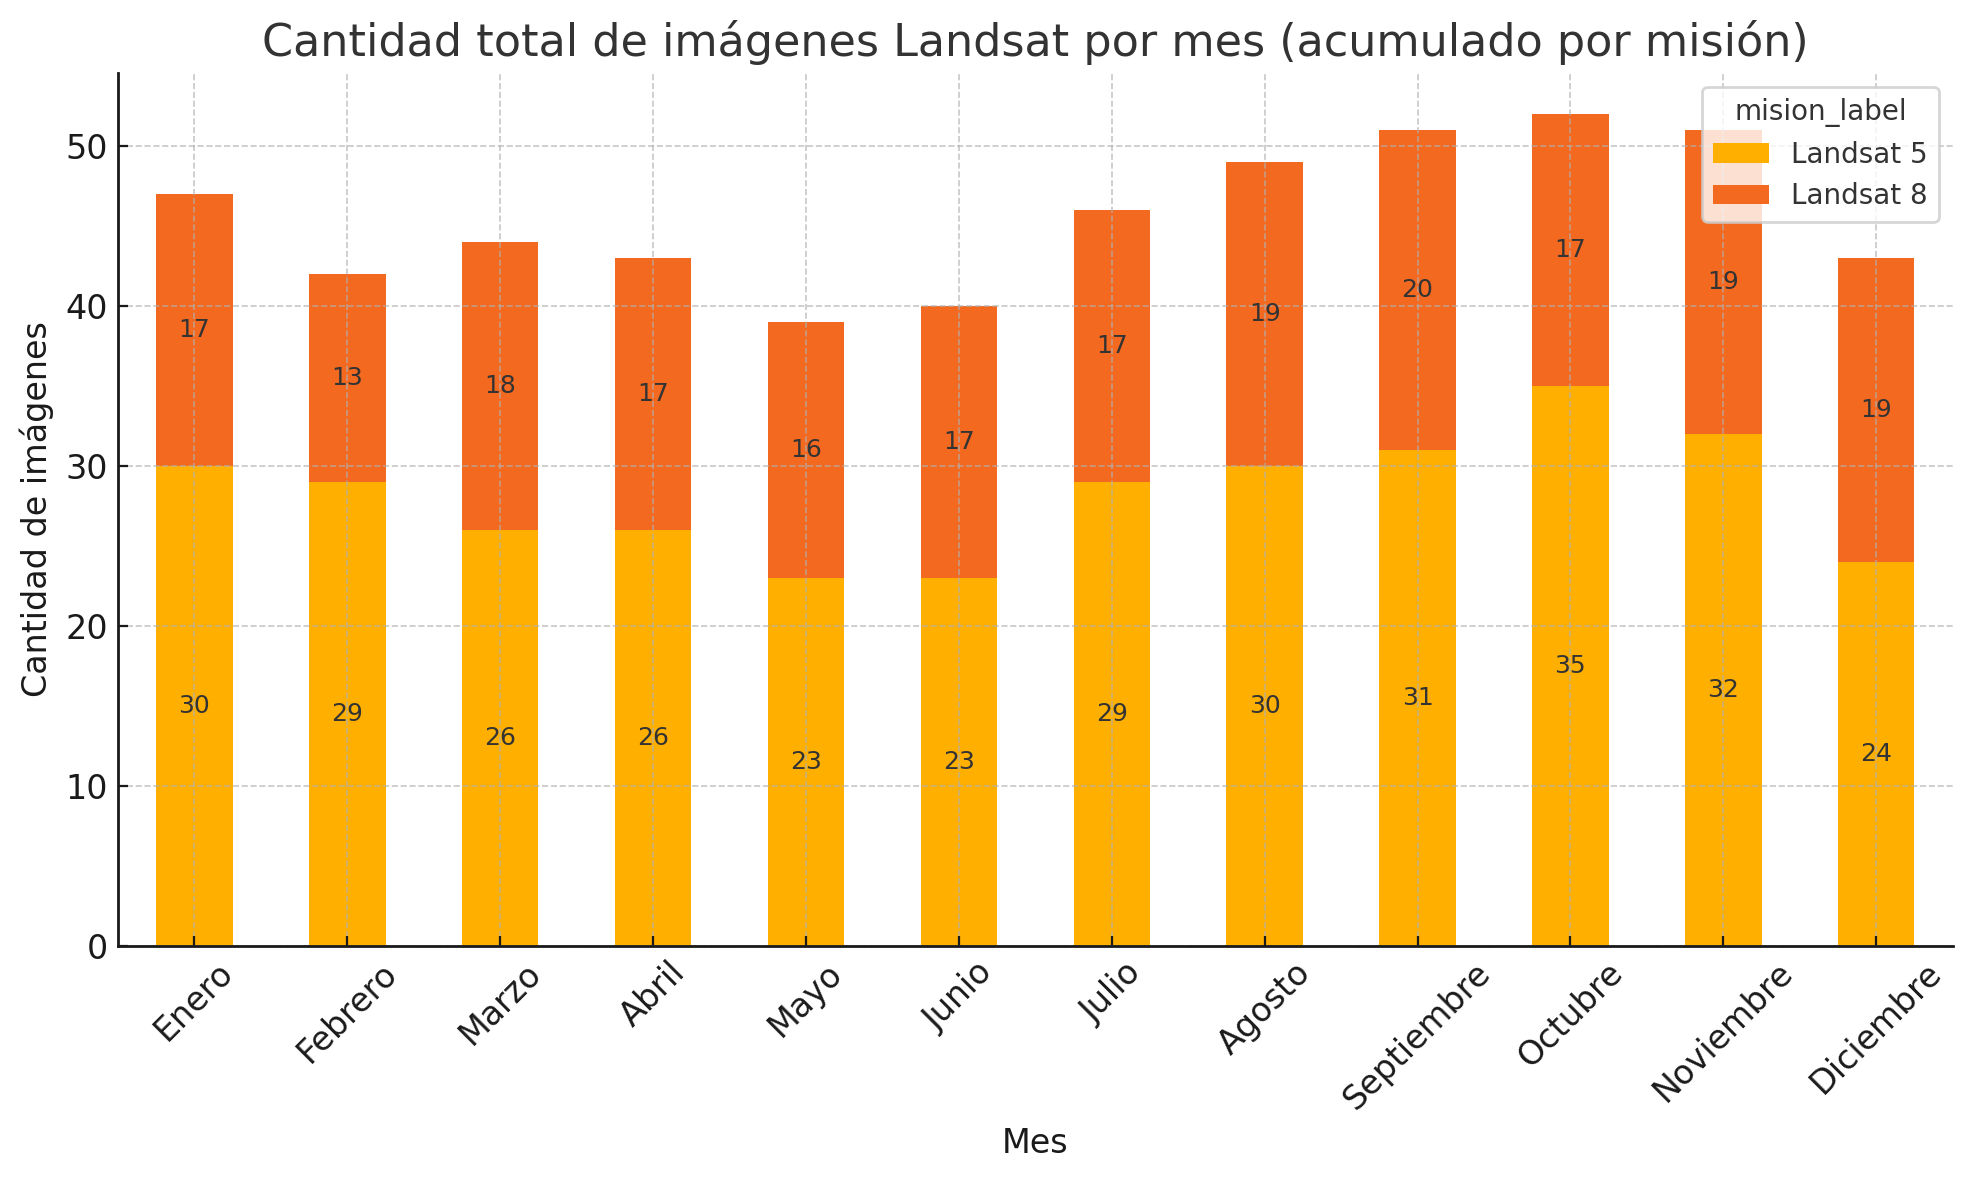
\includegraphics[scale=.4]
        {Figures/fig12.png}
        \caption{Cantidad de imágenes por mes y misión.}
        \label{fig:cant_imagenes}
\end{figure}

\subsection{Datos climáticos globales}

Como complemento a la información satelital, se integraron series temporales mensuales de los principales índices asociados al fenómeno ENSO. Estos indicadores ya han sido presentados en el Capítulo~\ref{Chapter2}; en esta sección se detalla únicamente el tratamiento aplicado para su incorporación en el análisis.

\begin{itemize}
    \item ONI (Oceanic Niño Index): se descargaron los valores mensuales publicados por la NOAA, calculados a partir de anomalías de temperatura superficial del mar en la región Niño 3.4 \parencite{noaaONI}. La serie fue recortada al período de análisis (1984--2022) y estandarizada mediante transformación a \textit{z-score}. Los resultados se muestran en la Figura~\ref{fig:indice_oni}.
    
    \item SOI (Southern Oscillation Index): se emplearon los datos mensuales provistos por el \textit{Australian Bureau of Meteorology} \parencite{bom_soi_2024}. La serie fue ajustada para coincidir en fechas con las observaciones de agua y normalizada con \textit{z-score}. La Figura~\ref{fig:indice_soi} presenta su evolución en el período de estudio.
    
    \item MEI.v2 (Multivariate ENSO Index, versión 2): se descargaron los valores bimestrales publicados por el NOAA Physical Sciences Laboratory \parencite{meiindex}. Para este trabajo, la serie se transformó a escala mensual asignando cada valor al segundo mes del par, y posteriormente se estandarizó con \textit{z-score}. En la Figura~\ref{fig:indice_mei} se ilustra la dinámica del índice.
\end{itemize}

De esta manera, las tres series ENSO quedaron homogeneizadas en frecuencia y escala, lo que permitió su comparación directa con la serie de área de agua superficial del Salar de Llullaillaco.




\section{Series de tiempo preliminares}

Todos los índices climáticos utilizados en este estudio (ONI, SOI y MEI) fueron estandarizados mediante su transformación a \textit{z-score} para facilitar la comparación entre series con distintas escalas y unidades. En la figura~\ref{fig:indice_area} se observa la evolución temporal del área de la laguna de estudio en \textit{z-score}, mientras que en las figuras~\ref{fig:indice_oni_ts},~\ref{fig:indice_soi_ts} y~\ref{fig:indice_mei_ts} se muestran los índices ONI, SOI y MEI en \textit{z-score} respectivamente.

\begin{figure}[ht]
        \centering
        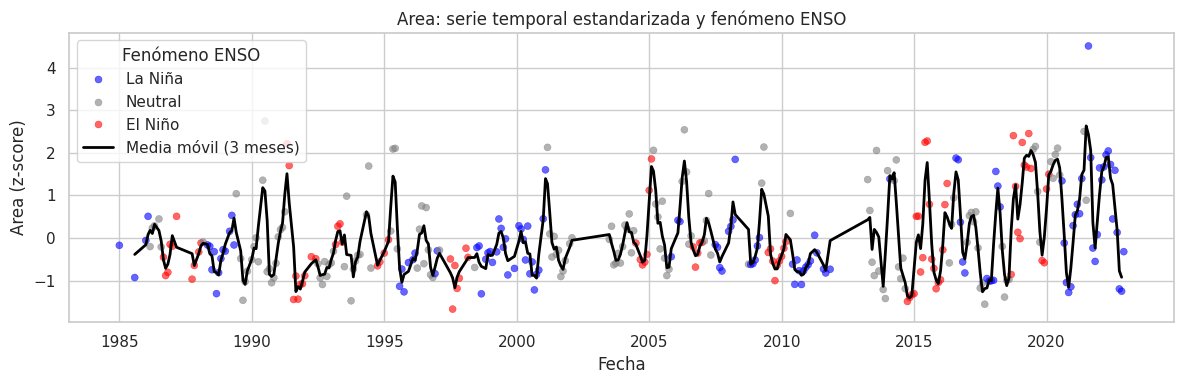
\includegraphics[scale=.45]
        {Figures/fig16_ts_area.png}
        \caption{Registro histórico de la variable Área (1984-2022).}
        \label{fig:indice_area}
\end{figure}



Se identificó que las series originales de cobertura de agua superficial y de los índices climáticos ENSO (ONI, SOI y MEI) no eran homogéneas, ya que presentaban vacíos temporales y diferencias en la disponibilidad de datos a lo largo del período de estudio. Esta heterogeneidad impedía su tratamiento directo como series de tiempo y, en consecuencia, limitaba la aplicación de algoritmos de \textit{machine learning} especializados en predicción temporal.  

Por ello, fue necesario realizar un proceso de estandarización y depuración de las series, ajustando su frecuencia y completitud para generar secuencias temporales comparables y aptas para los modelos predictivos. En la figura~\ref{fig:conteo_datos} se muestra la distribución de meses con datos disponibles por año para cada variable, lo que evidencia la falta de homogeneidad inicial. 

Posteriormente, se aplicaron técnicas de preprocesamiento y estrategias de imputación para obtener series homogéneas y continuas, que constituyen la base para el análisis de correlaciones y la construcción de modelos predictivos basados en series temporales.  

\section{Construcción de la serie temporal continua}

El primer paso consistió en evaluar la disponibilidad de imágenes por año y por variable 
derivada, lo que permitió identificar períodos con escasa cobertura. En particular, se 
consideraron como años incompletos aquellos con más de un 50\% de vacíos de información, 
es decir, con menos de seis meses de observaciones válidas en alguna de las series 
analizadas. Este diagnóstico reveló brechas significativas en ciertos intervalos, como 
el año 2012, donde no se registraron imágenes útiles.

A partir de este análisis se plantearon dos estrategias para construir una serie mensual 
continua de superficie de agua:

\begin{enumerate}
    \item Escenario estricto (descartar años incompletos): en este enfoque se 
    eliminaron directamente los años con cobertura insuficiente, priorizando la calidad 
    de los datos a costa de acortar la longitud de la serie temporal. 

    \item Estrategia híbrida de imputación: se diseñó un procedimiento de dos 
    etapas que permite conservar toda la serie completa entre 1984 y 2022: 
    \begin{itemize}
        \item Para brechas cortas (menores o iguales a cinco meses) se aplicó 
        interpolación temporal, de modo de mantener la coherencia local de las 
        observaciones.
        \item Para brechas largas (como años completos sin datos), se recurrió a 
        la imputación estacional, reemplazando los valores ausentes por el promedio 
        histórico de cada mes. De esta forma se preserva la estacionalidad propia de la 
        serie, evitando la introducción de sesgos por valores promedio anuales.
    \end{itemize}
\end{enumerate}


La estrategia híbrida permitió mantener la continuidad de la serie completa, a la vez 
que redujo el impacto de los vacíos extensos. Por su parte, el escenario estricto se 
conservó como ejercicio de sensibilidad metodológica, contrastando la robustez de los 
resultados frente a diferentes tratamientos de los faltantes. En la figura ~\ref{fig:ts_final} se muestran las series temporales resultantes.


\begin{figure}[ht]
        \centering
        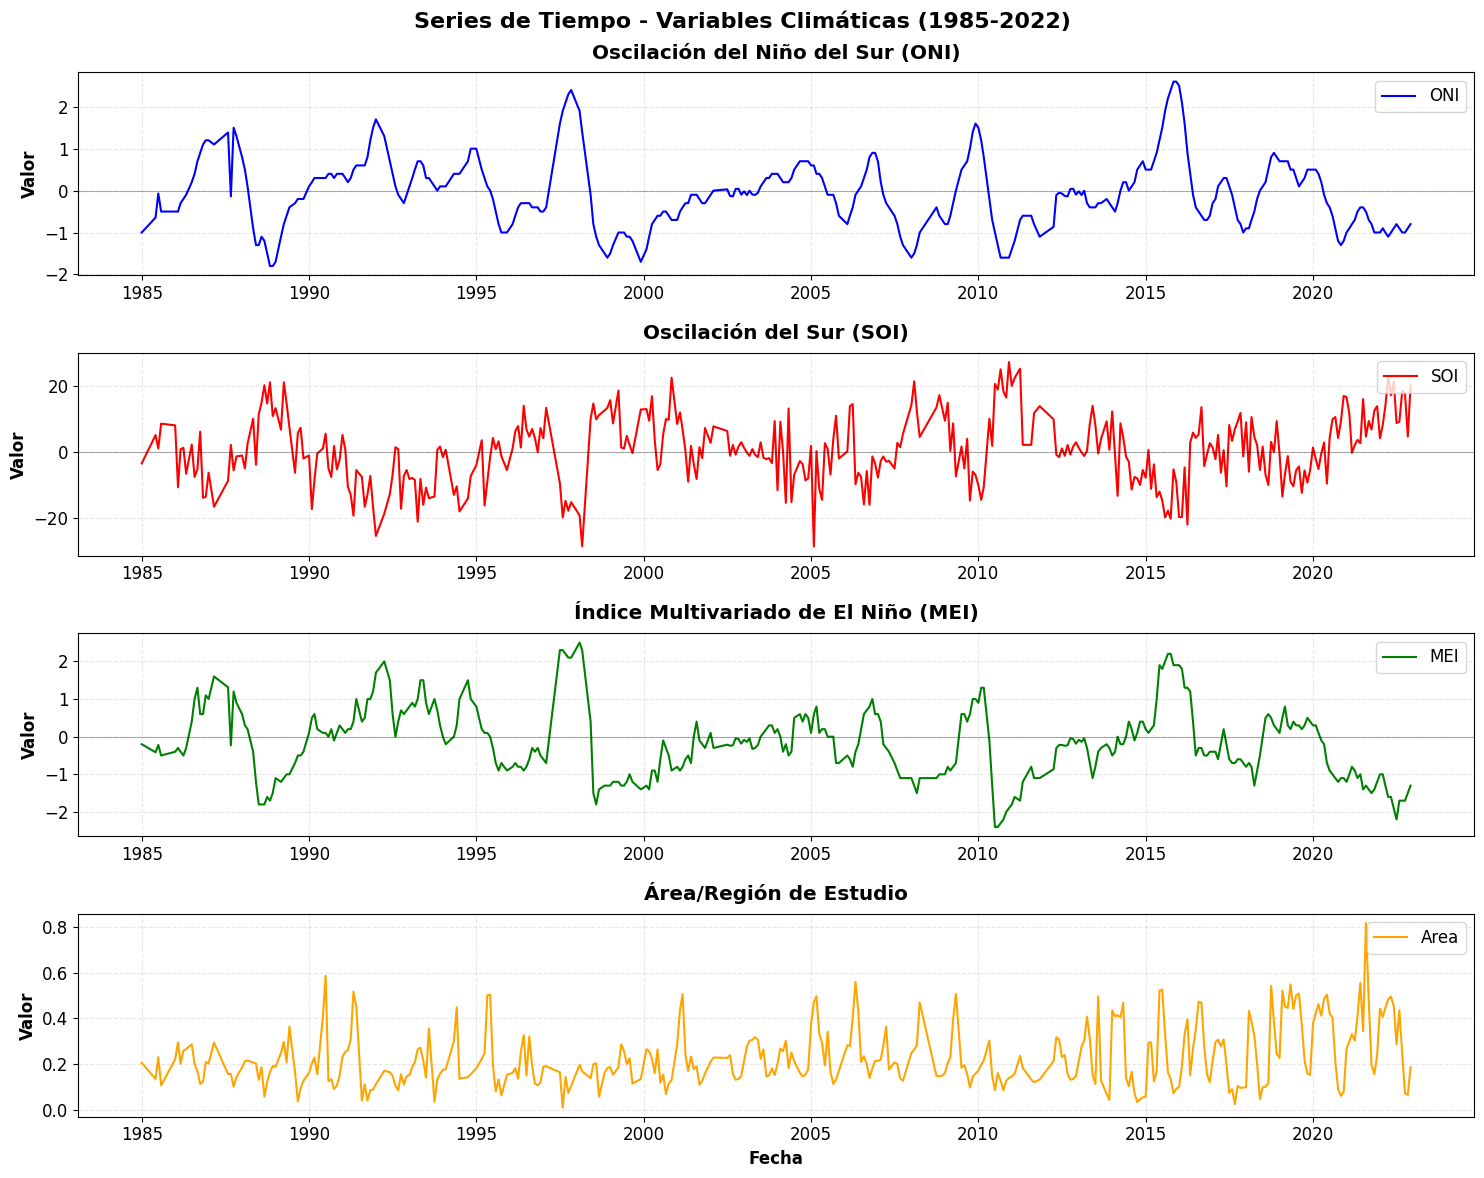
\includegraphics[scale=.32]
        {Figures/ts_final.png}
        \caption{Series temporales procesadas.}
        \label{fig:ts_final}
\end{figure}

\section{Exploración y tratamiento de las series temporales}
En esta sección se realiza una exploración de las variables a trabajar. Además, se realizan análisis visuales y comparaciones entre las variables. 

\subsection{Raíces unitarias}

Antes de la aplicación de modelos autorregresivos, se realizó un análisis visual de las 
series para explorar posibles tendencias o comportamientos no estacionarios. De manera 
preliminar, se observaron los siguientes patrones:

\begin{itemize}
    \item Serie Área (superficie de agua): muestra una tendencia descendente a lo 
    largo del período analizado, disminuyendo de valores cercanos a 0,8 hacia 0,2. Este 
    comportamiento sugiere la presencia de una deriva temporal y, por lo tanto, 
    no estacionariedad en media.
    \item Índices ENSO (ONI, SOI, MEI): presentan un comportamiento oscilatorio 
    alrededor de cero, sin tendencia ascendente o descendente clara y con variabilidad 
    relativamente constante. Estas características son típicas de series estacionarias.
\end{itemize}

Para corroborar estas observaciones se aplicó la prueba de Dickey-Fuller aumentada (ADF), cuyo objetivo es contrastar la hipótesis nula de no estacionariedad. La hipótesis nula se rechaza si el p-valor es menor a 0,05 o si el estadístico ADF es menor al valor crítico al 5\%. Los resultados obtenidos se presentan en la tabla~\ref{tab:adf_test}.

\begin{table}[H]
    \centering
    \caption{Resultados del test Dickey-Fuller aumentado (ADF)}.
    \label{tab:adf_test}
    \begin{tabular}{lccc}
        \toprule
        \textbf{Serie} & \textbf{Estadístico ADF} & \textbf{p-valor} & \textbf{Conclusión} \\
        \midrule
        ONI  & -6,5601 & 0,000000 & Estacionaria \\
        SOI  & -5,2308 & 0,000008 & Estacionaria \\
        MEI  & -5,2128 & 0,000008 & Estacionaria \\
        Área & -2,8901 & 0,046511 & Estacionaria (débil) \\
        \bottomrule
    \end{tabular}
\end{table}

Según los tests realizados es posible interpretar lo siguiente:   
\begin{itemize}
    \item ONI, SOI y MEI: resultaron fuertemente estacionarios, con p-valores 
    iguales a 0.000008 y estadísticos ADF muy por debajo de los valores críticos al 1\%. 
    Esto confirma su patrón oscilatorio estable alrededor de cero.
    \item Área: se ubicó en el límite de la estacionariedad, con un p-valor de 
    0,0465 y un estadístico ADF menor al valor crítico al 5\% pero no al 1\%. Aunque el 
    test formalmente indica estacionariedad, la tendencia descendente observada en la 
    inspección visual sugiere precaución, recomendándose aplicar diferenciación en los 
    modelos para obtener mayor robustez.
\end{itemize}


En síntesis, las series climáticas ONI, SOI y MEI no requieren diferenciación, mientras que 
la serie de Área, aunque marginalmente estacionaria según ADF, podría beneficiarse de 
una transformación adicional.

\subsection{Análisis visual de ACF y PACF}

Con el fin de explorar la estructura de dependencia temporal de cada serie, se graficaron 
las funciones de autocorrelación (ACF) y autocorrelación parcial (PACF). Estas funciones 
permiten identificar patrones de memoria temporal, evaluar la estacionariedad y orientar 
la selección de órdenes iniciales para modelos ARIMA o SARIMA \parencite{box2015time, hyndman2018forecasting}. 

\subsubsection{Variable ONI}

La ACF del ONI(~\ref{fig:facp_oni}) muestra un decaimiento lento y oscilatorio, típico de procesos con memoria 
larga y comportamiento cíclico (El Niño / La Niña). La PACF evidencia un corte abrupto 
tras los primeros rezagos (lag 1 o 2), lo que sugiere que un modelo autorregresivo de bajo 
orden (AR(1) o AR(2)) podría capturar adecuadamente su estructura.

\subsubsection{Variable SOI}

La ACF del SOI(~\ref{fig:facp_soi}) presenta un patrón de decaimiento oscilatorio persistente, con memoria de 
largo plazo. La PACF muestra un corte tras los primeros rezagos (lag 1–2), indicando que 
un modelo AR(2) constituye un buen punto de partida para esta serie.

\subsubsection{Variable MEI}

El MEI exhibe un patrón similar al ONI y SOI: la ACF(~\ref{fig:facp_mei}) decae lentamente con oscilaciones, 
mientras que la PACF se corta tras los primeros rezagos. Esto indica la presencia de 
dependencia temporal y ciclos ENSO, siendo un modelo AR(1)–AR(2) adecuado como 
aproximación inicial.

\subsubsection{Variable Área}

La ACF del Área (~\ref{fig:facp_area}) muestra un decaimiento muy lento y persistente, lo que refleja la 
presencia de una tendencia dominante y sugiere no estacionariedad. La PACF presenta un 
corte marcado en el lag 1, reforzando la necesidad de diferenciar la serie (I=1) antes de 
ajustar un modelo ARIMA. Tras la diferenciación, un modelo AR(1) constituye un punto de 
partida razonable.

\subsection{Resumen comparativo de ACF, PACF y estadísticos descriptivos}

Para complementar el análisis visual, se calcularon los primeros 10 rezagos de la función 
de autocorrelación (FAC) y la función de autocorrelación parcial (FACP) para cada serie. 
Asimismo, se presentan sus estadísticas descriptivas básicas. 

\begin{table}[H]
    \centering
    \caption{FAC en los primeros 3 rezagos.}
    \label{tab:fac}
    \begin{tabular}{lccc}
        \toprule
        \textbf{Serie} & \textbf{Lag 1} & \textbf{Lag 2} & \textbf{Lag 3} \\
        \midrule
        ONI  & 0,963 & 0,897 & 0,802 \\
        SOI  & 0,694 & 0,634 & 0,575 \\
        MEI  & 0,946 & 0,865 & 0,781 \\
        Área & 0,641 & 0,346 & 0,157 \\
        \bottomrule
    \end{tabular}
\end{table}

\begin{table}[H]
    \centering
    \caption{FACP en los primeros 3 rezagos.}
    \label{tab:facp}
    \begin{tabular}{lccc}
        \toprule
        \textbf{Serie} & \textbf{Lag 1} & \textbf{Lag 2} & \textbf{Lag 3} \\
        \midrule
        ONI  & 0,965 & -0,451 & -0,342 \\
        SOI  & 0,696 &  0,295 &  0,129 \\
        MEI  & 0,948 & -0,299 &  0,004 \\
        Área & 0,642 & -0,112 & -0,031 \\
        \bottomrule
    \end{tabular}
\end{table}


\begin{table}[H]
    \centering
    \caption{Estadísticos descriptivos de las series}.
    \label{tab:descriptivos}
    \begin{tabular}{lcccccc}
        \toprule
        Serie & Media & Desv. Est. & Mínimo & Q1 & Mediana & Máximo \\
        \midrule
        ONI   & -0,068 & 0,839 & -1,80 & -0,70 & -0,10 &  2,60 \\
        SOI   &  0,394 & 10,168 & -28,6 & -6,30 &  0,60 & 27,10 \\
        MEI   & -0,150 & 0,952 & -2,40 & -0,87 & -0,22 &  2,50 \\
        Área  &  0,222 & 0,120 &  0,01 &  0,14 &  0,19 &  0,82 \\
        \bottomrule
    \end{tabular}
\end{table}


De acuerdo a los resultados precedentes es posible resumir las métricas en lo siguiente:
\begin{itemize}
    \item ONI: La FAC presenta autocorrelación muy fuerte en los primeros rezagos 
    (0,96 en lag 1), confirmando memoria persistente y patrón oscilatorio. La PACF muestra 
    un corte abrupto tras el lag 1–2, lo que sugiere un modelo autorregresivo de bajo orden 
    (AR(1)–AR(2)).
    
    \item SOI: También evidencia fuerte dependencia temporal, con FAC significativa 
    hasta varios rezagos y PACF con corte en lag 1–2. Sus valores extremos y desviación 
    estándar elevada (±10) confirman alta variabilidad climática. Un modelo AR(2) es adecuado 
    como punto de partida.
    
    \item MEI: Exhibe un comportamiento casi idéntico al ONI, con FAC alta en los 
    primeros rezagos (0,95 en lag 1) y PACF con caída tras lag 1–2. Esto refleja la estructura 
    oscilatoria de ENSO. Un modelo AR(1)–AR(2) es consistente.
    
    \item Área: Aunque la FAC arranca alta (0.64), decae rápidamente con rezagos, 
    sugiriendo fuerte tendencia de fondo. La PACF muestra un pico en lag 1 y caída posterior, 
    lo que indica necesidad de diferenciación (I=1) antes de ajustar un modelo ARIMA. La media 
    baja (0,22) y la dispersión estrecha confirman que los cambios son más lentos y dominados 
    por tendencia descendente.
\end{itemize}




Como conclusión general, se puede mencionar que las series climáticas (ONI, SOI, MEI) muestran 
estacionariedad con memoria corta, modelables con AR(1)–AR(2). En contraste, la serie 
Área no es estacionaria y requiere diferenciación previa; tras este paso, un modelo AR(1) 
o SARIMA con estacionalidad anual resulta más adecuado.

\subsection{Tratamiento de la serie Área mediante diferenciación}

Dado que la serie Área presentó una clara tendencia y solo una estacionariedad débil según 
el test ADF, se aplicó una primera diferenciación (I=1) para eliminar la deriva temporal. 
El análisis posterior de autocorrelación mostró un comportamiento mucho más estable, con 
valores de FAC y FACP cercanos a cero en los primeros rezagos, y ausencia de patrones de 
dependencia prolongada.

\begin{figure}[H]
    \centering
    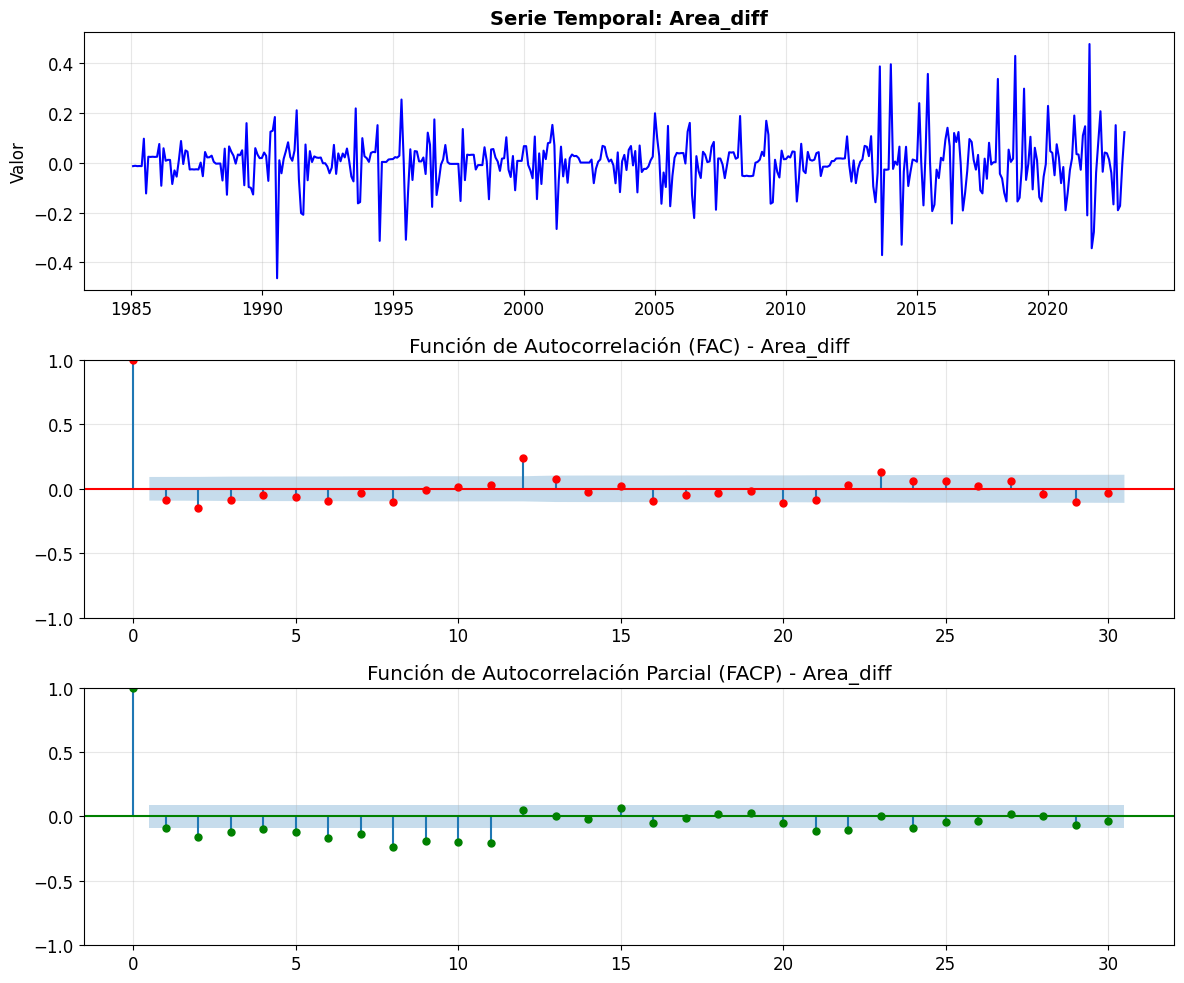
\includegraphics[scale=.42]{Figures/facp_Area_dif.png}
    \caption{Funciones ACF y PACF de la serie Área (superficie de agua).}
    \label{fig:facp_area_dif}
\end{figure}

\begin{table}[H]
    \centering
    \caption{Resultados de pruebas de estacionariedad aplicadas a Área\_diff.}
    \label{tab:ru_area_diff}
    \begin{tabular}{lccc}
        \toprule
        \textbf{Prueba} & \textbf{Estadístico} & \textbf{p-valor} & \textbf{Conclusión} \\
        \midrule
        Dickey-Fuller Aumentada (ADF) & -14,8466 & 0,0000 & Estacionaria \\
        KPSS & 0,0239 & 0,1000 & Estacionaria \\
        Phillips-Perron (PP) & -33,5219 & 0,0000 & Estacionaria \\
        \bottomrule
    \end{tabular}
\end{table}

Las tres pruebas (ADF, KPSS y PP) coinciden en rechazar la hipótesis de no estacionariedad, 
confirmando que la serie diferenciada es estacionaria. Este resultado valida la 
necesidad del preprocesamiento y garantiza que la serie Área\_diff puede ser utilizada en 
modelos ARIMA o SARIMA con mayor robustez. 




% Chapter Template

\chapter{Ensayos y resultados} % Main chapter title

\label{Chapter4} % Change X to a consecutive number; for referencing this chapter elsewhere, use \ref{ChapterX}
En este capítulo se presentan los resultados obtenidos de los ensayos realizados, los cuales incluyen, pero no se limitan a: resultado de la segmentación CNN U-Net. para la obtención de la serie temporal de superficie de agua de la laguna, resultados de modelado SARIMA para todas las series temporales estudiadas, resultado del modelado VAR y por último los resultados de la aplicación de rolling forecasting a las variables área. 

%----------------------------------------------------------------------------------------
%	SECTION 1
%----------------------------------------------------------------------------------------

\section{Segmentación mensual con U-Net: resultados operativos}

La segmentación automática de cuerpos de agua se implementó con una arquitectura U-Net \citep{ronneberger2015unet} entrenada bajo el esquema \textit{student–teacher} \citep{hinton2015distilling}. El objetivo fue obtener una serie mensual continua de cobertura de agua superficial, evitando la necesidad de etiquetado manual masivo. Para ello, se empleó un 5\% de las imágenes del cubo temporal mensual, generando las etiquetas a partir del NDWI umbralizado ($>0,15$). El modelo resultante se aplicó a la totalidad de imágenes del período 1984–2022.

\subsection{Curvas de entrenamiento y validación}
En la figura~\ref{fig:unet_training} se muestran las curvas de entrenamiento y validación de la red U-Net, utilizando como función de pérdida la \textit{Binary Cross Entropy} (BCE). Se observa una disminución rápida de la pérdida durante las primeras 15 épocas, seguida de una convergencia estable hacia valores próximos a cero. La similitud entre las curvas de entrenamiento y validación indica un buen equilibrio entre ajuste y generalización, sin evidencias de sobreajuste. El mejor desempeño en validación se alcanzó en la época 78, lo que confirma la capacidad del modelo para segmentar de manera consistente las áreas de agua a partir de las imágenes Landsat.

\begin{figure}[H]
    \centering
    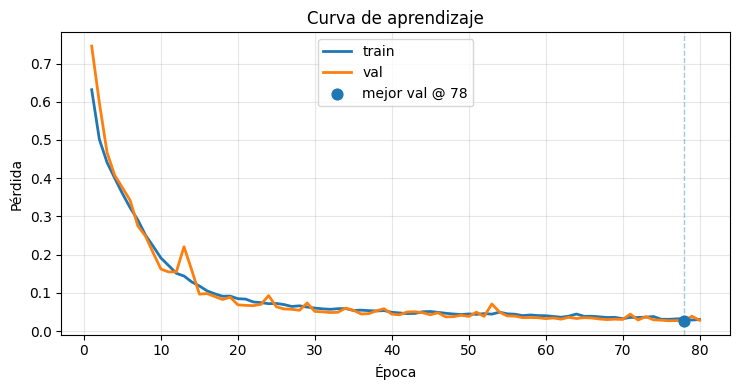
\includegraphics[scale=0.55]{Figures/curva_entrenamiento.png}
    \caption{Curvas de entrenamiento y validación de la U-Net.}
    \label{fig:unet_training}
\end{figure}

\subsection{Ejemplos de segmentación}
La figura~\ref{fig:unet_examples} muestra ejemplos representativos de la segmentación mensual: a la izquierda las imágenes Landsat en composición RGB de falso color, y a la derecha las máscaras binarias generadas por la U-Net. Se aprecia coherencia espacial en la identificación de cuerpos de agua, con detección consistente de la laguna central y reducción de falsos positivos respecto de umbrales simples de NDWI.

\begin{figure}[H]
    \centering
    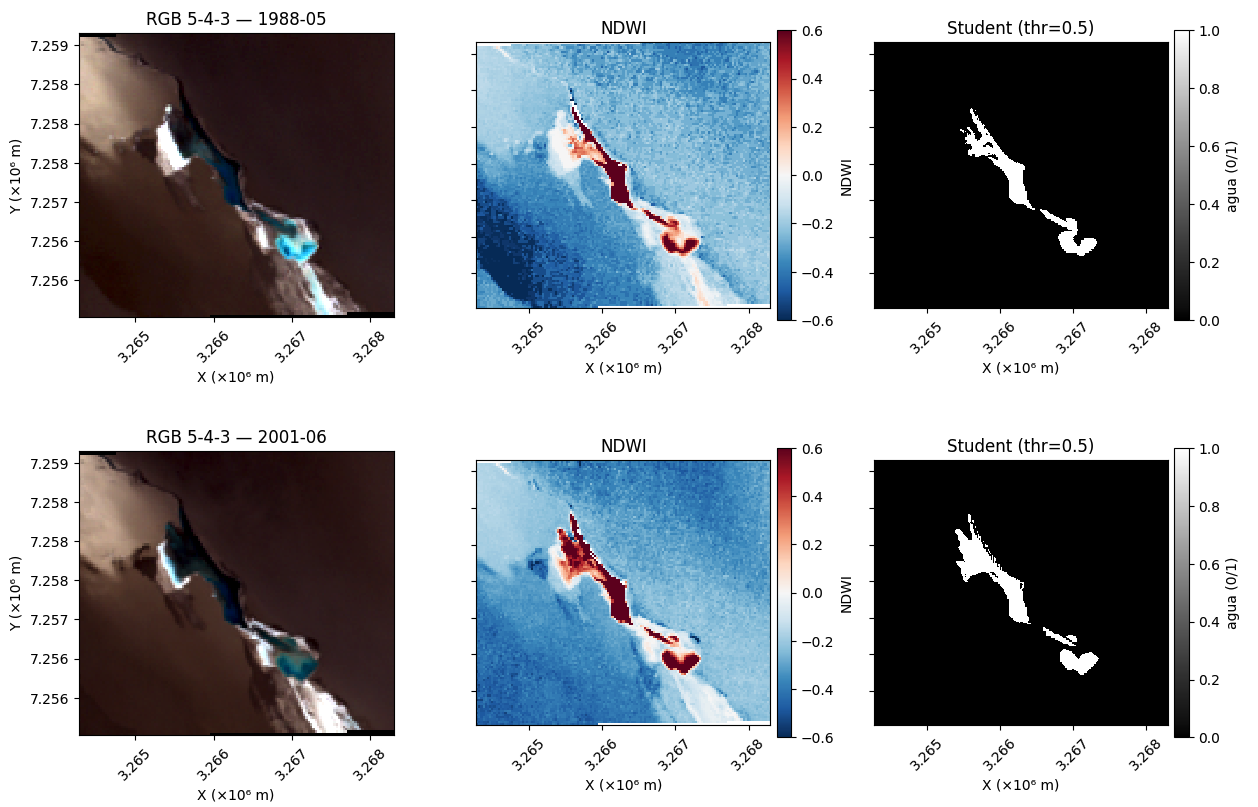
\includegraphics[scale=0.32]{Figures/unet_examples.png}
    \caption{Ejemplos de segmentación mensual: comparación entre imágenes Landsat (falso color) y máscaras U-Net.}
    \label{fig:unet_examples}
\end{figure}

\subsection{Consistencia temporal}
La figura ~\ref{fig:ts_final} ilustra la serie temporal del área de agua derivada de la segmentación U-Net. La dinámica temporal reproduce patrones estacionales y anomalías coherentes con la climatología regional, validando la estabilidad del procedimiento. Esta serie constituye la base de los modelos de predicción temporal desarrollados en las secciones SARIMA.

\subsection{Probabilidad mensual de agua}

A partir del cubo temporal clasificado con la U-Net se calculó, para cada mes del período de análisis, la probabilidad de ocurrencia de agua. Este cálculo se realizó como la proporción de píxeles clasificados como agua sobre el total de píxeles de la laguna en el mes correspondiente. De esta manera, se obtuvo una serie temporal mensual de probabilidades que permite evaluar la consistencia del modelo y la dinámica hidrológica en escalas estacionales e interanuales.

En la figura~\ref{fig:prob_agua_mensual} se presenta un ejemplo gráfico de estos resultados. Se observa la variabilidad temporal de la probabilidad de agua, con máximos que coinciden con períodos de mayor extensión superficial y mínimos en fases de retracción. Este producto constituye un insumo clave para la modelización temporal desarrollada en los capítulos siguientes, pues resume la dinámica de la laguna en una métrica probabilística derivada de la clasificación automática.

\begin{figure}[H]
    \centering
    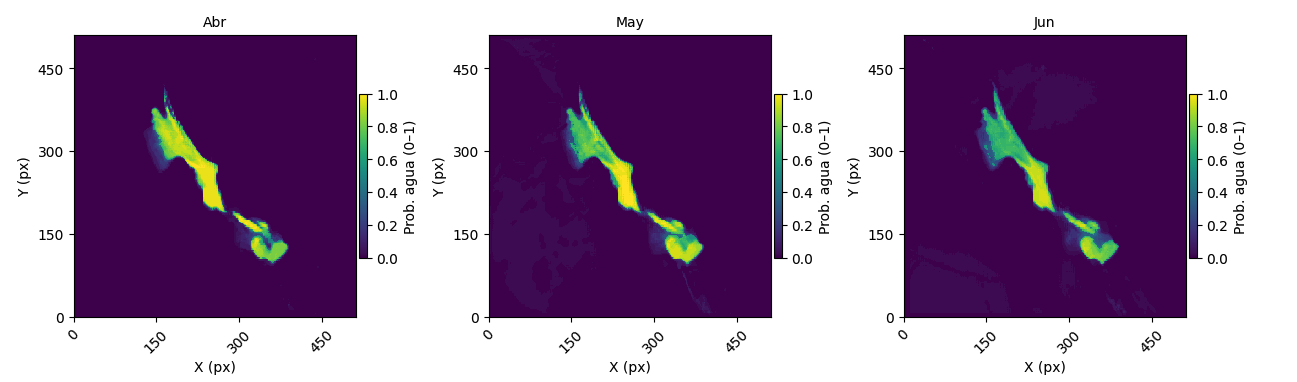
\includegraphics[scale=0.31]{Figures/prob_agua1.png}
    \caption{Probabilidad mensual de ocurrencia de agua en la laguna Llullaillaco, derivada de la segmentación U-Net.}
    \label{fig:prob_agua_mensual}
\end{figure}

\begin{figure}[H]
    \centering
    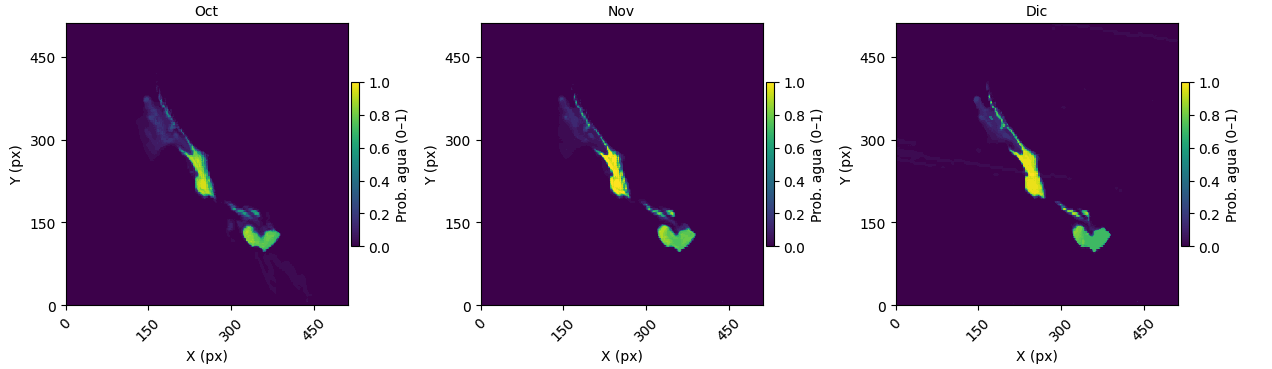
\includegraphics[scale=0.31]{Figures/prob_agua2.png}
    \caption{Probabilidad mensual de ocurrencia de agua en la laguna Llullaillaco, derivada de la segmentación U-Net.}
    \label{fig:prob_agua_mensual2}
\end{figure}

\section{Modelado con SARIMA}

El modelo SARIMA (\textit{Seasonal ARIMA}) fue optimizado para cada una de las series de interés (ONI, SOI, MEI y Área), evaluando diferentes combinaciones de parámetros $(p,d,q)\times(P,D,Q,s)$ y seleccionando los mejores ajustes según el criterio de información de Akaike (AIC). 

\subsection{ONI}
El mejor modelo seleccionado para ONI fue SARIMA$(2,0,1)\times(1,1,2)_{12}$, con un AIC de $-410.64$. Este modelo supera en desempeño a alternativas cercanas como SARIMA$(2,0,2)\times(1,1,2)_{12}$ y SARIMA$(2,0,0)\times(1,1,2)_{12}$, confirmando que la estructura óptima incluye un componente autorregresivo de orden 2 y un componente de media móvil de orden 1.

\subsection{SOI}
En el caso de SOI, el mejor modelo corresponde a SARIMA$(1,0,2)\times(2,1,2)_{12}$, con un AIC de $2842.34$. Aunque este valor absoluto es elevado (debido a la alta varianza intrínseca de la serie), la comparación relativa muestra que es la configuración más adecuada frente a otras alternativas con órdenes similares.

\subsection{MEI}
La serie MEI fue mejor explicada por SARIMA$(2,0,2)\times(1,1,2)_{12}$, alcanzando un AIC de $126.37$. Este modelo captura tanto la persistencia como los patrones estacionales de la serie, y presenta una ventaja clara frente a otros candidatos como SARIMA$(1,0,1)\times(1,1,2)_{12}$ y SARIMA$(2,0,1)\times(1,1,2)_{12}$.

\subsection{Área y Área\_diff}
Para la serie Área sin diferenciar, el mejor modelo fue SARIMA$(1,0,0)\times(1,0,1)_{12}$ con un AIC de $-902.08$. Sin embargo, al diferenciar la serie (Área\_diff), se obtuvo como mejor ajuste el modelo SARIMA$(2,0,1)\times(1,0,1)_{12}$ con un AIC de $-888.19$. Aunque el AIC es ligeramente menos favorable tras la diferenciación, los análisis de raíces unitarias y métricas de predicción (ver subsección anterior) mostraron que el modelo diferenciado ofrece mayor robustez y estacionariedad.

\begin{table}[H]
    \centering
    \caption{Resumen de los mejores modelos SARIMA seleccionados por serie.}
    \begin{tabular}{lccc}
        \toprule
        \textbf{Serie} & \textbf{Mejor modelo SARIMA} & \textbf{AIC} & \textbf{Notas} \\
        \midrule
        ONI   & $(2,0,1)\times(1,1,2)_{12}$ & $-410.64$ & Estacionalidad marcada \\
        SOI   & $(1,0,2)\times(2,1,2)_{12}$ & $2842.34$ & Alta varianza residual \\
        MEI   & $(2,0,2)\times(1,1,2)_{12}$ & $126.37$  & Buen equilibrio AR y MA \\
        Área  & $(1,0,0)\times(1,0,1)_{12}$ & $-902.08$ & No diferenciada \\
        Área\_diff & $(2,0,1)\times(1,0,1)_{12}$ & $-888.19$ & Estacionaria, mayor robustez \\
        \bottomrule
    \end{tabular}
    \label{tab:sarima_modelos}
\end{table}

En síntesis, el procedimiento de optimización permitió identificar configuraciones distintas para cada serie, adaptadas a sus características temporales. En los siguientes apartados se evaluará la performance predictiva de estos modelos sobre los conjuntos de test.

\section{Evaluación de los modelos SARIMA}

Se evaluó el desempeño predictivo de los modelos SARIMA seleccionados para las series
ONI, SOI, MEI, \emph{Área} y \emph{Área\_diff}, considerando: métricas de error en el
conjunto de test (MSE, MAE, RMSE y MAPE cuando aplica), diagnóstico de residuos
(residuos en el tiempo, ACF/PACF de residuos, normalidad aproximada y test de Ljung--Box),
y parsimonia y significancia de coeficientes (AIC/BIC, $p$--valores).

\subsection{Criterios de diagnóstico}
Se consideró que un modelo es adecuado cuando:
\begin{itemize}
    \item los residuos no presentan autocorrelación remanente (ACF/PACF dentro de bandas y Ljung--Box con $p>0.05$),
    \item no hay patrones sistemáticos en los residuos,
    \item las métricas de error son coherentes con la escala de la serie,
    \item la parametrización es parsimoniosa (sin términos innecesarios o no significativos).
\end{itemize}

\subsection{Resultados por serie y diagnóstico}
Se incluyen los siguientes gráficos de diagnóstico, los cuales pueden verse en el Apéndice de figuras:

\begin{itemize}
    \item Residuos en el tiempo.  
    \item Funciones de autocorrelación (ACF) y autocorrelación parcial (PACF) de los residuos.  
    \item Histograma, densidad y gráfico Q--Q.  
    \item Gráfico de p--valores de la prueba de Ljung--Box por rezago.  
    \item Serie observada (train+test) versus predicciones con intervalo de confianza al 95\%.  
\end{itemize}

\subsubsection{ONI} 
Modelo SARIMA$(2,0,1)\times(1,1,2)_{12}$ (AIC $\approx -410.6$). 
Los coeficientes no estacionales AR(2) y MA(1) son altamente significativos y capturan la
dinámica de corto plazo; sin embargo, los términos estacionales no resultan
significativos. El test Jarque--Bera rechaza normalidad y se observa heterocedasticidad,
pero los residuos no presentan autocorrelación relevante. En test: 
MSE $=0.683$, MAE $=0.631$, RMSE $=0.826$. En las figuras~\ref{fig:res_oni} y~\ref{fig:pred_oni} se pueden apreciar los residuos del modelo y las predicciones para el conjunto de test.

Conclusión: buen ajuste de la dinámica no estacional; recomendable
simplificar la parte estacional (evaluar ARIMA$(2,0,1)$ sin estacionalidad) y re‐chequear
residuos.
\vspace{0.3em}




\subsubsection{SOI}
Modelo SARIMA$(1,0,2)\times(2,1,2)_{12}$ (AIC $\approx 2116$).
AR(1), MA(1) y varios términos estacionales son significativos. MA(2) y AR estacional en
$24$ meses no son significativos. Residuos sin autocorrelación (Ljung--Box con $p>0.05$) y con leve
no normalidad. En test: MSE $=88.00$, MAE $=7.64$, RMSE $=9.38$. En las figuras~\ref{fig:res_soi} y~\ref{fig:pred_soi} se pueden apreciar los residuos del modelo y las predicciones para el conjunto de test.

Conclusión: desempeño predictivo insuficiente para la escala del SOI. Es conveniente simplificar y eliminar términos no significativos además de explorar transformaciones robustas.
\vspace{0.3em}


\subsubsection{MEI}
Modelo SARIMA$(2,0,2)\times(1,1,2)_{12}$ (AIC $\approx 126.4$).
AR(1), AR(2) y MA(1) no estacionales son muy significativos. El modelo MA(2) es marginal. 
En la parte estacional sólo AR a 12 meses es relevante. Los términos MA estacionales no lo son.
Residuos sin autocorrelación (Ljung--Box con $p\approx 0,84$), con colas algo pesadas.
En test: MSE $=0,821$, MAE $=0,725$, RMSE $=0,906$. En las figuras~\ref{fig:res_mei} y~\ref{fig:pred_mei} se pueden apreciar los residuos del modelo y las predicciones para el conjunto de test.

Conclusión: buen comportamiento predictivo. En trabajos futuros seria oportuno simplificar
la estacionalidad (p.\,ej., SARIMA$(2,0,1)\times(1,1,0)_{12}$) y verificar residuos.
\vspace{0.3em}


\subsubsection{Área (sin diferenciar)}
Modelo SARIMA$(1,0,0)\times(1,0,1)_{12}$ 
(AIC $\approx -902.1$). Todos los coeficientes son significativos; el término AR estacional
es muy alto ($\approx 0.996$), lo que sugiere posible necesidad de diferenciación
estacional. Los residuos no presentan autocorrelación, aunque con no normalidad.
En test: MSE $=0,02499$, MAE $=0,119$, RMSE $=0,158$. En las figuras~\ref{fig:res_area} y~\ref{fig:pred_area} se pueden apreciar los residuos del modelo y las predicciones para el conjunto de test.

Conclusión: buen ajuste en escala de la serie; aun así, la magnitud de AR estacional sugiere evaluar un $D=1$ para mayor estabilidad.
\vspace{0.3em}


\subsubsection{Área\_diff (diferenciada)}
Modelo SARIMA$(2,0,1)\times(1,0,1)_{12}$
(AIC $\approx -888.2$). Los residuos presentan comportamiento de ruido blanco (ACF/PACF dentro
de bandas, Ljung--Box con $p>0,05$), normalidad aproximada y métricas de error muy bajas:
MSE $=0.01782$, MAE $=0,0910$, RMSE $=0,1335$, MAPE $=1,70\%$. En las figuras~\ref{fig:res_area_d} y~\ref{fig:pred_area_d} se pueden apreciar los residuos del modelo y las predicciones para el conjunto de test.

Conclusión:buen desempeño y mayor robustez estadística tras la diferenciación esto valida el preprocesamiento efectuado (ver sección de raíces unitarias).


En la tabla~\ref{tab:metricas_sarima} se pueden observar las métricas para los modelos SARIMA para variables analizadas. 

\begin{table}[H]
\centering
\caption{Resumen de métricas de desempeño en test para modelos SARIMA}
\label{tab:metricas_sarima}
\begin{tabular}{lcccc}
\toprule
\textbf{Serie} & \textbf{MSE} & \textbf{MAE} & \textbf{RMSE} & \textbf{MAPE} \\
\midrule
ONI  & 0,683  & 0,631  & 0,826  & n/a \\
SOI  & 88,003 & 7,639  & 9,381  & n/a \\
MEI  & 0,821  & 0,725  & 0.906  & n/a \\
Área (sin diff) & 0,02499 & 0,1190 & 0,1581 & n/a \\
Área\_diff      & \textbf{0,01782} & \textbf{0,0910} & \textbf{0,1335} & \textbf{1,70\%} \\
\bottomrule
\end{tabular}
\end{table}

Como resultado de la aplicación del modelo SARIMA en las series temporales a continuación se sintetizan los principales hallazgos.

\begin{itemize}
    \item Series ENSO (ONI, MEI): los componentes AR(2) y MA(1) no estacionales
    capturan bien la memoria de corto plazo; varios términos MA estacionales no son
    significativos. .
    \item Serie SOI: los residuos no muestran autocorrelación, las métricas de la precisión predictiva son altas.
    \item Series Área vs. Área\_diff: ambos modelos presentan muy buen desempeño en test,
    destacándose \emph{Área\_diff} con los errores más bajos y residuos más
    estables.
\end{itemize}

En conjunto, la evidencia empírica muestra que la diferenciación de la serie \emph{Área}
mejora la robustez y precisión del modelo, mientras que en las series ENSO una
parametrización más parsimoniosa tiende a ser suficiente. El caso SOI requiere trabajo
adicional para alcanzar niveles de error aceptables.

\section{Modelado VAR (Vectores Autorregresivos)}

El modelo VAR (\textit{Vector AutoRegressive}) es una técnica de series temporales multivariadas que permite capturar las interdependencias entre varias variables a lo largo del tiempo. A diferencia de los modelos univariados como ARIMA o SARIMA, el VAR considera que cada variable del sistema depende no solo de sus propios valores pasados, sino también de los valores pasados de las demás variables incluidas en el modelo \parencite{lutkepohl2005new}.

El análisis VAR constituye la base para explorar relaciones causales entre las variables y evaluar la capacidad predictiva conjunta del sistema.

\subsection{Prueba de Causalidad de Granger}

La prueba de causalidad de Granger evalúa si los valores pasados de una serie temporal contienen información útil para predecir otra serie, bajo el supuesto de relaciones lineales dentro de un modelo VAR \parencite{granger1969investigating}.
La hipótesis nula (\(H_0\)) establece que “la serie X no causa Granger a la serie Y”. Un p-valor inferior a 0,05 permite rechazar la hipótesis nula, concluyendo que existe causalidad grangeriana.

En este estudio, se aplicó la prueba con un máximo de 24 rezagos mensuales, obteniéndose la matriz de resultados presentada en la tabla~\ref{tab:granger_matrix}.

\begin{table}[H]
    \centering
    \caption{Matriz de p-valores de la prueba de causalidad de Granger (máx. 24 rezagos).}
    \label{tab:granger_matrix}
    \begin{tabular}{lcccc}
        \toprule
        & ONI\_x & SOI\_x & MEI\_x & Área\_x \\
        \midrule
        ONI\_y  & 0,9999   & 0,1189   & 0,0142$^{*}$ & 0,1057   \\
        SOI\_y  & 0,0000$^{*}$ & 1,0000   & 0,0000$^{*}$ & 0,0410$^{*}$ \\
        MEI\_y  & 0,0000$^{*}$ & 0,0000$^{*}$ & 1,0000   & 0,3261   \\
        Área\_y & 0,5889   & 0,0456$^{*}$ & 0,4557   & 1,0000   \\
        \bottomrule
    \end{tabular}
        
\end{table}

A continuación se presenta una sintesis de los principales hallazgos obtenidos por la prueba de causalidad de Granger.
\begin{itemize}
    \item ONI\_y: sólo es causado por el MEI (p=0,014), lo que indica que la información del índice multivariado MEI contribuye a predecir al ONI.
    \item SOI\_y: recibe causalidad de ONI, MEI y el Área, reflejando su carácter central como índice atmosférico.
    \item MEI\_y: es causado por ONI y SOI, lo que confirma la fuerte interdependencia entre los índices climáticos de ENSO.
    \item Área\_y: solo es causada por el SOI (p=0,046), lo que evidencia que la variabilidad atmosférica influye directamente en la superficie de agua del salar.
\end{itemize}


El análisis de causalidad de Granger confirma la interdependencia entre los tres índices climáticos (ONI, SOI, MEI), coherente con la naturaleza multivariada del ENSO. Entre ellos, el SOI emerge como el índice más influyente, pues no solo se ve afectado por ONI y MEI, sino que además es el único que causa variaciones significativas en el área de agua superficial. Este hallazgo refuerza la hipótesis de que la dinámica atmosférica vinculada al SOI constituye un modulador clave de la hidrología altoandina.

\subsection{Modelo VAR: selección del orden y resultados}

Para modelar la dinámica conjunta entre los índices ENSO (ONI, SOI, MEI) y la superficie de agua (Área), se ajustó un modelo VAR (Vector Autorregresivo). A diferencia de los modelos univariados como ARIMA o SARIMA, el VAR permite capturar relaciones dinámicas multivariadas, considerando que cada variable depende tanto de sus propios rezagos como de los rezagos de las demás variables del sistema \cite{lutkepohl2005new}.

\subsubsection{Selección del orden de rezagos}
Se evaluaron los criterios de información AIC, BIC, HQIC y FPE para determinar el número óptimo de rezagos (tabla~\ref{tab:var_lags}). Los resultados muestran que el rezago $p=3$ minimiza la mayoría de los criterios (AIC, HQIC y FPE), por lo que se seleccionó un modelo VAR(3).

\begin{table}[H]
    \centering
    \caption{Selección del orden de rezagos para el modelo VAR.}
    \label{tab:var_lags}
    \begin{tabular}{lcccc}
        \toprule
        \textbf{Rezago} & \textbf{AIC} & \textbf{BIC} & \textbf{HQIC} & \textbf{FPE} \\
        \midrule
        2 & -7,485 & -7,130$^\ast$ & -7,345 & 0,0005612 \\
        3 & -7,617$^\ast$ & -7,104 & -7,414$^\ast$ & 0,0004921$^\ast$ \\
        \bottomrule
    \end{tabular}
\end{table}

El ajuste del modelo mostró que:

\begin{itemize}
    \item ONI presenta un fuerte componente autoregresivo, con significancia en los rezagos 1 y 3, lo que confirma su persistencia temporal.
    \item SOI depende de sus propios rezagos, pero también recibe influencia significativa del ONI, reforzando los vínculos entre estos índices ENSO.
    \item MEI es explicado principalmente por sus propios rezagos, aunque también recibe influencia de ONI y SOI.
    \item El Área muestra alta dependencia de su propio rezago inmediato (L1.Area $\approx 0,67$), lo que indica fuerte persistencia temporal. Además, se observa una influencia marginal de SOI (p$\approx 0,05$), consistente con la prueba de causalidad de Granger.
\end{itemize}

Por otra parte, la matriz de correlación entre los residuos (tabla~\ref{tab:var_corr_resid}) muestra que:

\begin{itemize}
    \item ONI y MEI presentan una correlación positiva alta (0,59), consistente con la interdependencia observada en los coeficientes.
    \item SOI mantiene correlaciones negativas con ONI (-0,23) y MEI (-0,45), reforzando su rol como índice atmosférico diferenciado.
    \item El Área muestra correlaciones débiles con el resto de variables, lo que indica que sus residuos son relativamente independientes.
\end{itemize}


\begin{table}[H]
    \centering
    \caption{Matriz de correlación de los residuos del modelo VAR(3).}
    \label{tab:var_corr_resid}
    \begin{tabular}{lcccc}
        \toprule
               & ONI & SOI & MEI & Área \\
        \midrule
        ONI     & 1,000 & -0,232 &  0,590 &  0,068 \\
        SOI     & -0,232 & 1,000 & -0,454 & -0,094 \\
        MEI     & 0,590 & -0,454 &  1,000 &  0,066 \\
        Área    & 0,068 & -0,094 &  0,066 &  1,000 \\
        \bottomrule
    \end{tabular}
\end{table}

Por ultimo, se aplicó el test de normalidad basado en asimetría y curtosis. La hipótesis nula (H$_0$: residuos con distribución normal) fue rechazada al 5\% de significancia (p-valor=0.000). Esto indica que los residuos no son normales, presentando colas pesadas y asimetrías, una situación común en series climáticas y ambientales. Aunque no compromete la validez del VAR, sí implica que los intervalos de confianza deben interpretarse con cautela.

\subsubsection{Predicciones}
En la figura~\ref{fig:var_pred} se presentan las predicciones del modelo VAR comparadas con los valores observados. Se observa que el modelo logra capturar adecuadamente la evolución de ONI y MEI, mientras que en SOI las oscilaciones extremas resultan más difíciles de reproducir. En el caso del Área, las predicciones se mantienen dentro de un rango consistente, aunque con menor variabilidad que la observada.

\subsubsection{Respuestas al impulso}
Las funciones de respuesta al impulso (IRF) permiten evaluar cómo un shock en una variable afecta a las demás dentro del sistema (figura~\ref{fig:var_irf}). Los resultados indican que:

\begin{itemize}
    \item Un shock positivo en ONI genera efectos persistentes en sí mismo y también incrementa los valores de MEI.
    \item Un shock en SOI produce impactos negativos significativos sobre ONI y MEI, además de afectar el Área en los primeros periodos.
    \item El Área responde principalmente a perturbaciones de SOI, lo que refuerza su rol como variable climática clave que influye en la superficie de agua.
\end{itemize}


\begin{figure}[H]
    \centering
    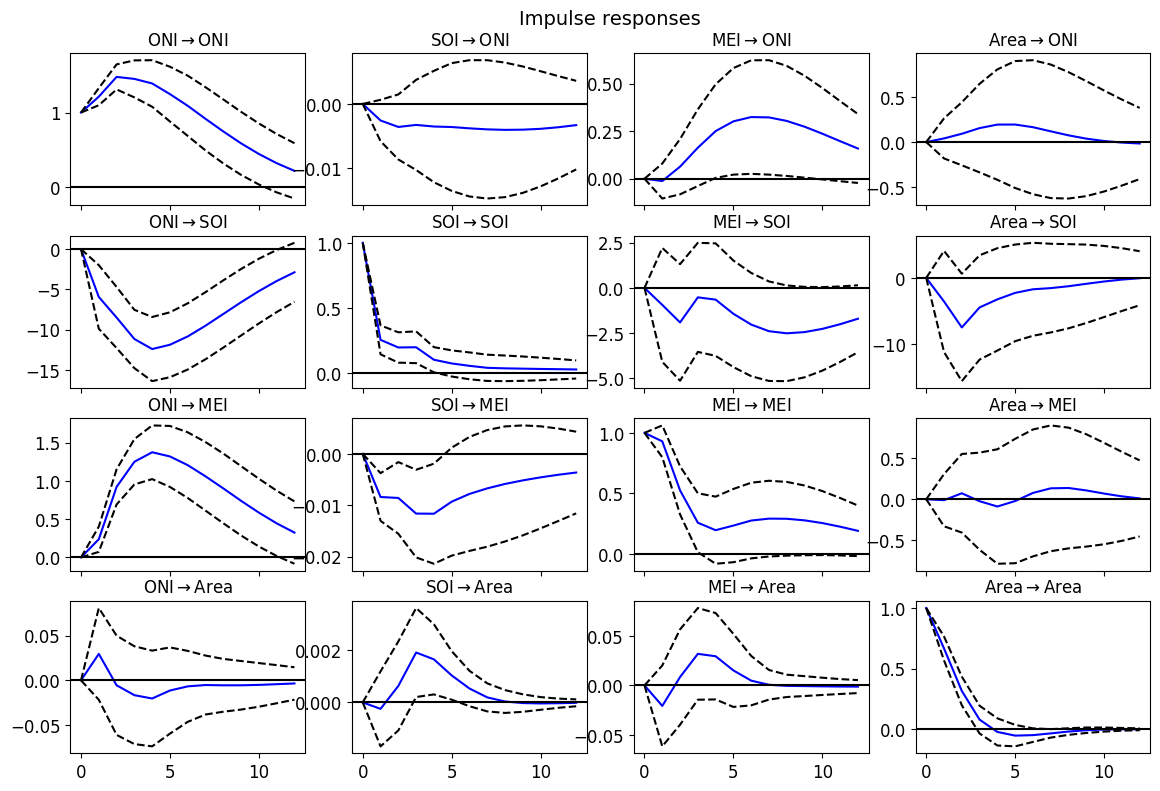
\includegraphics[scale=0.45]{Figures/var_ir.png}
    \caption{Funciones de respuesta al impulso (IRF) para el modelo VAR(3).}
    \label{fig:var_irf}
\end{figure}

\subsubsection{Conclusión parcial}
El modelo VAR(3) confirma la fuerte interrelación entre los índices ENSO (ONI, SOI, MEI) y muestra que la superficie de agua está particularmente influenciada por el SOI. Este resultado es consistente con la prueba de causalidad de Granger y con la lógica climática subyacente: la variabilidad atmosférica medida por el SOI tiene un efecto directo en la dinámica hidrológica del sistema estudiado. No obstante, la no normalidad de los residuos sugiere que futuros trabajos deberían considerar modelos más robustos (ej. VAR-GARCH o VAR con errores no gaussianos).


%----------------------------------------------------------------------------------------
%   SECTION 6: PRONÓSTICO ROLLING
%----------------------------------------------------------------------------------------

\section{Pronóstico rolling con SARIMA y VAR}

El pronóstico rolling permite evaluar la capacidad de los modelos para anticipar la evolución de las series en horizontes múltiples, actualizando el ajuste en cada paso con el valor observado. Este enfoque es más exigente que un pronóstico estático, ya que refleja el desempeño del modelo en un escenario de proyección operativa.

\subsection{Resultados con SARIMA}

La figura~\ref{fig:rolling_sarima} muestra el rolling forecast para la serie de Área. Se observa que el modelo sigue la dinámica general, aunque presenta limitaciones en la captura de picos abruptos.

\begin{itemize}
    \item MSE: 0,0133
    \item MAE: 0,0794
    \item RMSE: 0,1151
    \item MAPE: 43,07\%
\end{itemize}

Estos valores muestran un error moderado en términos absolutos (RMSE bajo), pero un MAPE elevado debido a la presencia de valores cercanos a cero, donde el porcentaje de error se amplifica.

\begin{figure}[H]
    \centering
    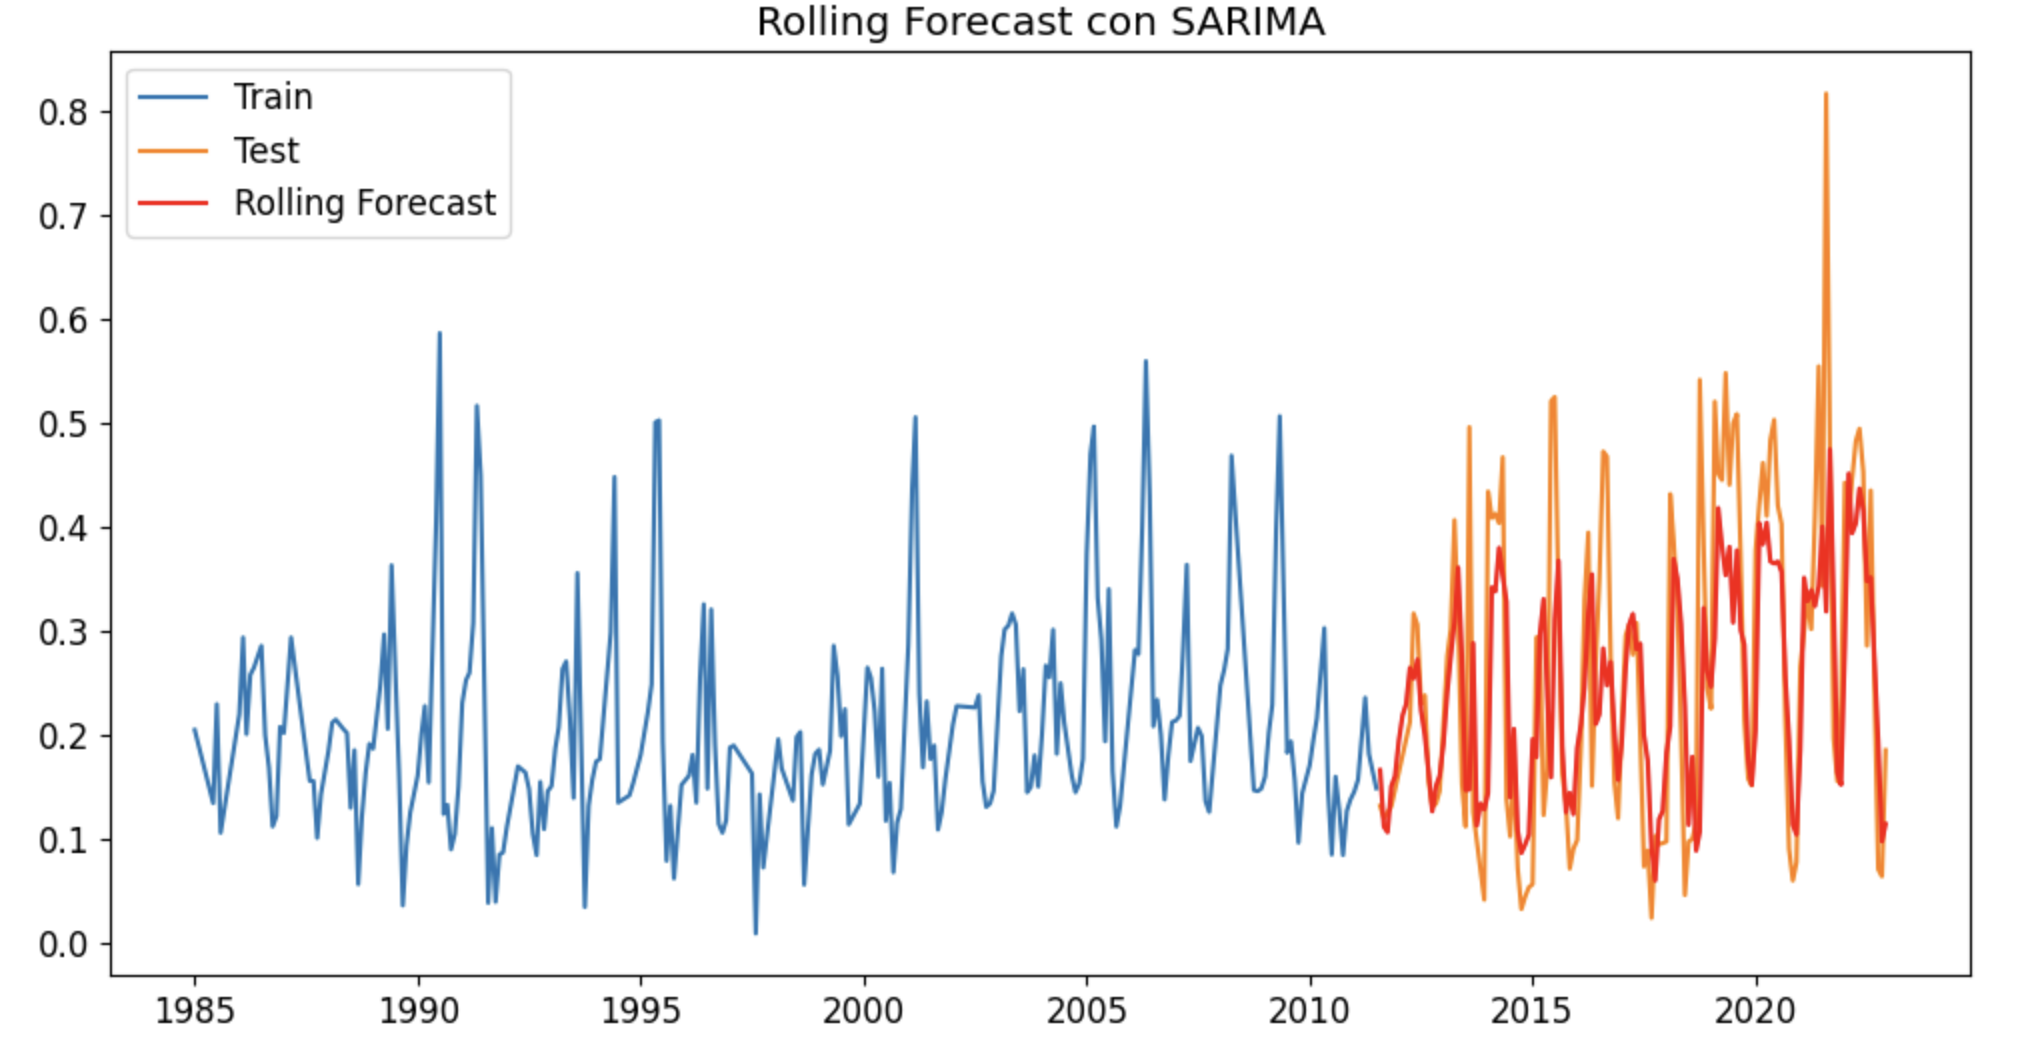
\includegraphics[scale=0.35]{Figures/rolling_sarima.png}
    \caption{Pronóstico rolling con SARIMA para la serie de Área.}
    \label{fig:rolling_sarima}
\end{figure}

\subsection{Resultados con VAR}

El modelo VAR fue evaluado para ONI, SOI, MEI y Área, con horizonte rolling de tres rezagos (figura~\ref{fig:rolling_var}).

\begin{itemize}
    \item MSE: 0,0176
    \item MAE: 0,0990
    \item RMSE: 0,1327
    \item MAPE: 45,58\%
\end{itemize}

\begin{figure}[H]
    \centering
    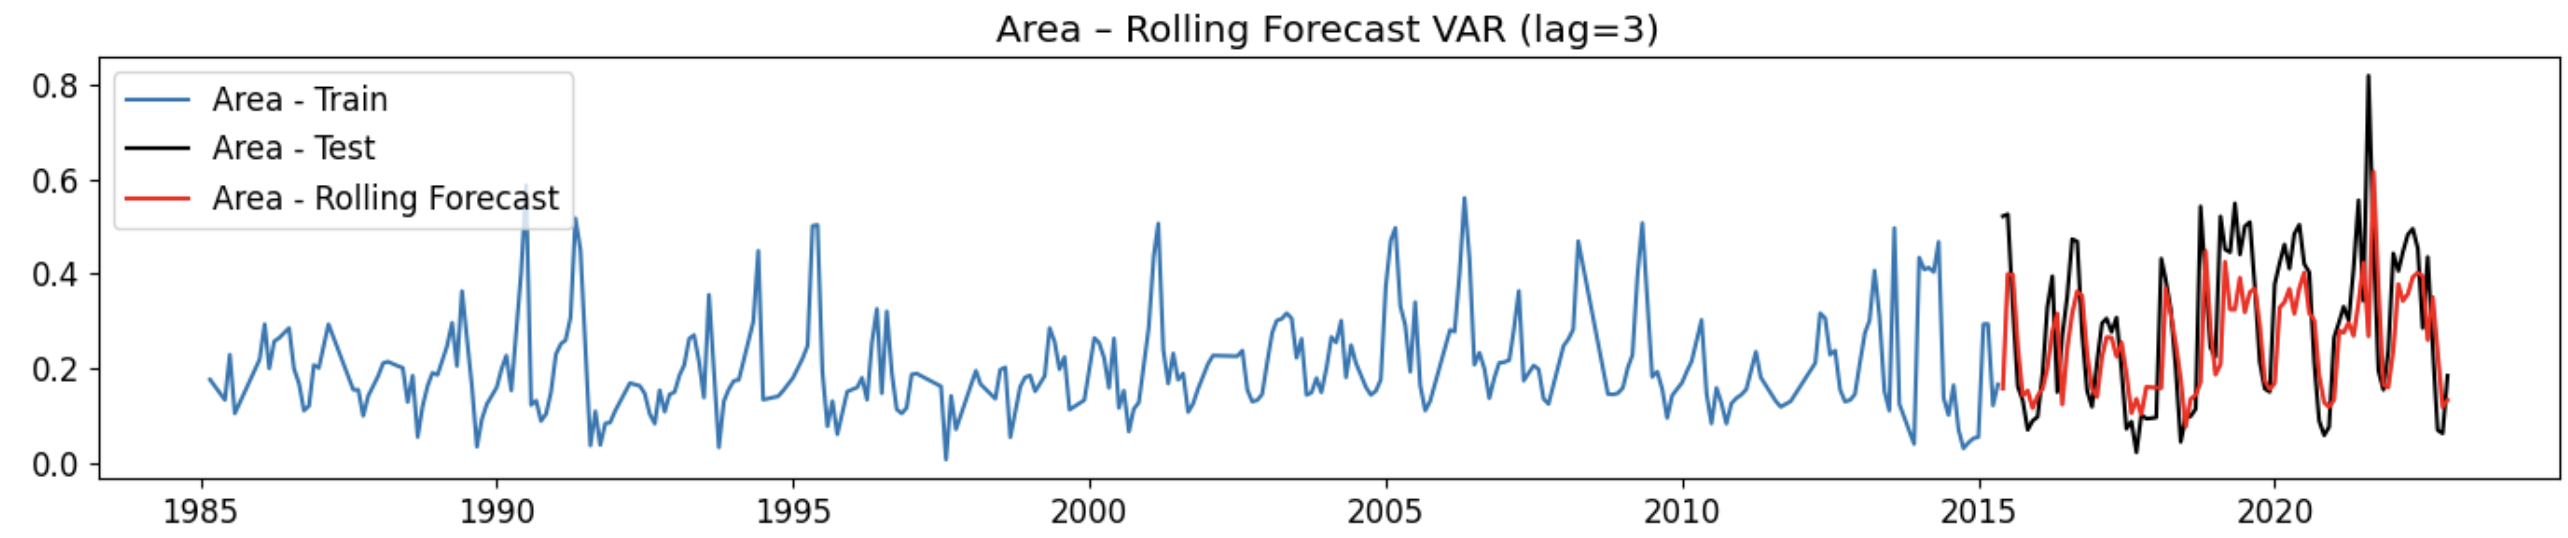
\includegraphics[scale=0.30]{Figures/rolling_var.png}
    \caption{Pronóstico rolling con SARIMA para la serie de Área..}
    \label{fig:rolling_var}
\end{figure}

\subsection{Comparación del desempeño en la serie Área}
La comparación de las métricas de la serie Área entre SARIMA y VAR muestra que ambos métodos alcanzan un desempeño satisfactorio, aunque con diferencias claras. El modelo SARIMA obtiene errores menores en todas las métricas (MSE = 0,0133; RMSE = 0,1151) frente al VAR (MSE = 0,0176; RMSE = 0,1327), lo que indica una mayor precisión en la predicción puntual. Asimismo, el MAE y el MAPE confirman la superioridad de SARIMA, reflejando que en promedio sus estimaciones se ajustan mejor a la magnitud real de la superficie de agua. No obstante, el VAR sigue mostrando un nivel de predicción aceptable, con la ventaja de modelar simultáneamente las interrelaciones con los índices ENSO, lo que lo convierte en una herramienta complementaria para analizar la dinámica conjunta del sistema climático-hidrológico.
\begin{table}[H]
    \centering
    \caption{Comparación de métricas para la serie Área entre SARIMA y VAR}
    \label{tab:comp_area}
    \begin{tabular}{lcccc}
        \toprule
        Método & MSE & MAE & RMSE & MAPE \\
        \midrule
        SARIMA & 0,0133 & 0,0794 & 0,1151 & 43,07\% \\
        VAR    & 0,0176 & 0,0990 & 0,1327 & 45,58\% \\
        \bottomrule
    \end{tabular}
\end{table}


\subsection{Pronóstico espacio–temporal con CNN (U-Net temporal)}

Con el fin de extender el análisis hacia el futuro, se desarrolló un modelo de redes neuronales convolucionales capaz de predecir la presencia de agua en la laguna a partir de imágenes satelitales mensuales. Para ello se utilizó una variante de la arquitectura U-Net \parencite{ronneberger2015unet}, adaptada para trabajar con secuencias de meses consecutivos en lugar de imágenes aisladas. De esta manera, el modelo aprovecha tanto la información espacial (formas y patrones dentro de cada imagen) como la temporal (cómo evoluciona el agua de un mes a otro).

El procedimiento consiste en entregarle al modelo un bloque de meses previos y pedirle que estime la máscara de agua del mes siguiente. Al repetir este proceso de manera encadenada (lo que se conoce como pronóstico autoregresivo), se obtiene una proyección de la dinámica de la laguna hacia adelante en el tiempo. Las salidas del modelo son tanto mapas de probabilidad de presencia de agua como máscaras binarias (agua/no agua) tras aplicar un umbral.

El entrenamiento se realizó con las series históricas de imágenes ya procesadas y normalizadas. Para evaluar su desempeño, se analizaron las curvas de pérdida en entrenamiento y validación, que mostraron una reducción estable a lo largo de las épocas. En los resultados cualitativos se observa que las predicciones del modelo reproducen coherentemente la forma y extensión de la laguna en distintos meses, mientras que la serie de área pronosticada mantiene la variabilidad temporal observada en los datos reales.

En síntesis, este enfoque basado en aprendizaje profundo permite no sólo reconstruir el pasado de manera automática, sino también generar escenarios futuros de disponibilidad de agua en el salar, lo que constituye un aporte novedoso respecto a los métodos estadísticos utilizados en las secciones anteriores.

\begin{figure}[H]
    \centering
    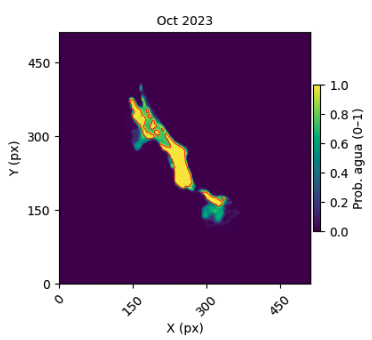
\includegraphics[scale=0.80]{Figures/forecast_cnn1.png}
    \caption{Pronóstico del área usando CNN (Octubre 2023).}
    \label{fig:forecast_cnn}
\end{figure}




\begin{figure}[H]
    \centering
    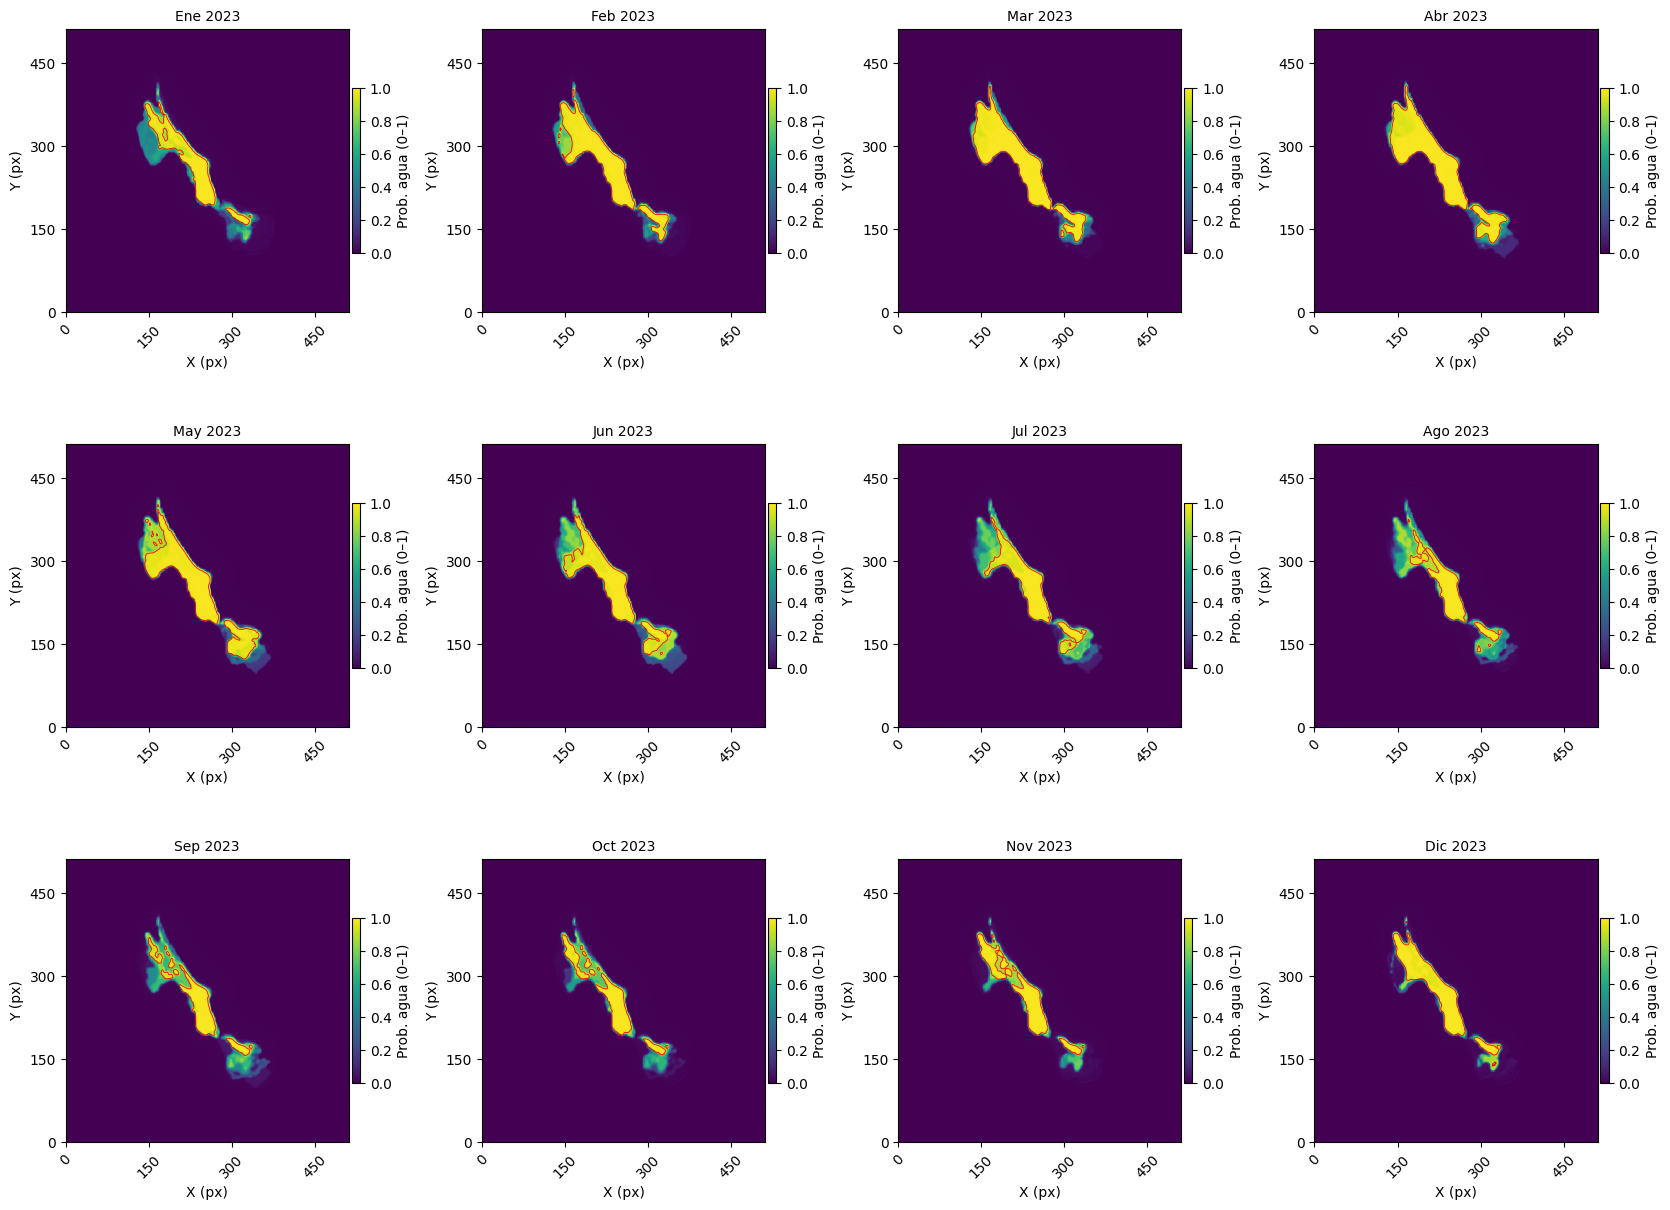
\includegraphics[scale=0.30]{Figures/forecast_cnn.png}
    \caption{Pronóstico del área usando CNN (12 meses.}
    \label{fig:forecast_cnn}
\end{figure}

\subsection{Arquitectura de la U-Net temporal}

La arquitectura implementada corresponde a una variante de U-Net \parencite{ronneberger2015unet}, diseñada originalmente para segmentación de imágenes biomédicas y hoy ampliamente utilizada en visión por computadora. En este trabajo se adaptó la red para integrar información espacio--temporal, de manera que no solo procese la forma y extensión de la laguna en cada mes, sino también la dinámica que muestran las secuencias mensuales previas.

La estructura general sigue un esquema de codificador--decodificador. En la primera parte (codificador), las imágenes de entrada ---una ventana temporal de varios meses consecutivos--- se reducen progresivamente en tamaño espacial mientras aumentan en profundidad, extrayendo representaciones de mayor nivel que capturan texturas, bordes y patrones espaciales. En la segunda parte (decodificador), la red reconstruye la resolución original combinando estas representaciones profundas con las características locales preservadas en las capas iniciales (conexiones tipo \emph{skip}). Esta estrategia permite mantener el detalle espacial de la laguna a la vez que se incorporan las dependencias temporales de la serie.

La salida de la red es un mapa bidimensional de probabilidad de presencia de agua para el mes siguiente. Dicho mapa puede umbralizarse para obtener una máscara binaria agua/no agua, o interpretarse directamente como una probabilidad espacial continua. En este trabajo se empleó una función de pérdida compuesta que combina \emph{binary cross entropy} y \emph{dice loss}, equilibrando la precisión en la clasificación pixel a pixel con la coherencia en la forma segmentada.

En la figura~\ref{fig:curva_unet} se presentan las curvas de pérdida durante el entrenamiento de la U-Net temporal. Se observa un descenso inicial pronunciado en las primeras épocas (1--5), donde la pérdida de entrenamiento disminuye de manera marcada, evidenciando la rápida captura de patrones relevantes. De forma consistente, la pérdida de validación también se reduce, indicando que el modelo logra generalizar a los datos no vistos.

A partir de la época 6, ambas curvas muestran una meseta con pequeñas oscilaciones, estabilizándose en torno a valores de $0.14$ para la validación y $0.087$--$0.089$ para el entrenamiento. La brecha entre ambas es reducida, lo que sugiere que no se presentan problemas significativos de sobreajuste. 

En síntesis, el modelo alcanzó un buen equilibrio entre aprendizaje y generalización, con resultados estables y consistentes. Como trabajo futuro, podrían explorarse ajustes finos (mayor número de épocas, uso de \emph{learning rate schedulers} o variación del \emph{batch size}) para mejorar aún más la estabilidad de la validación.

\begin{figure}[H]
    \centering
    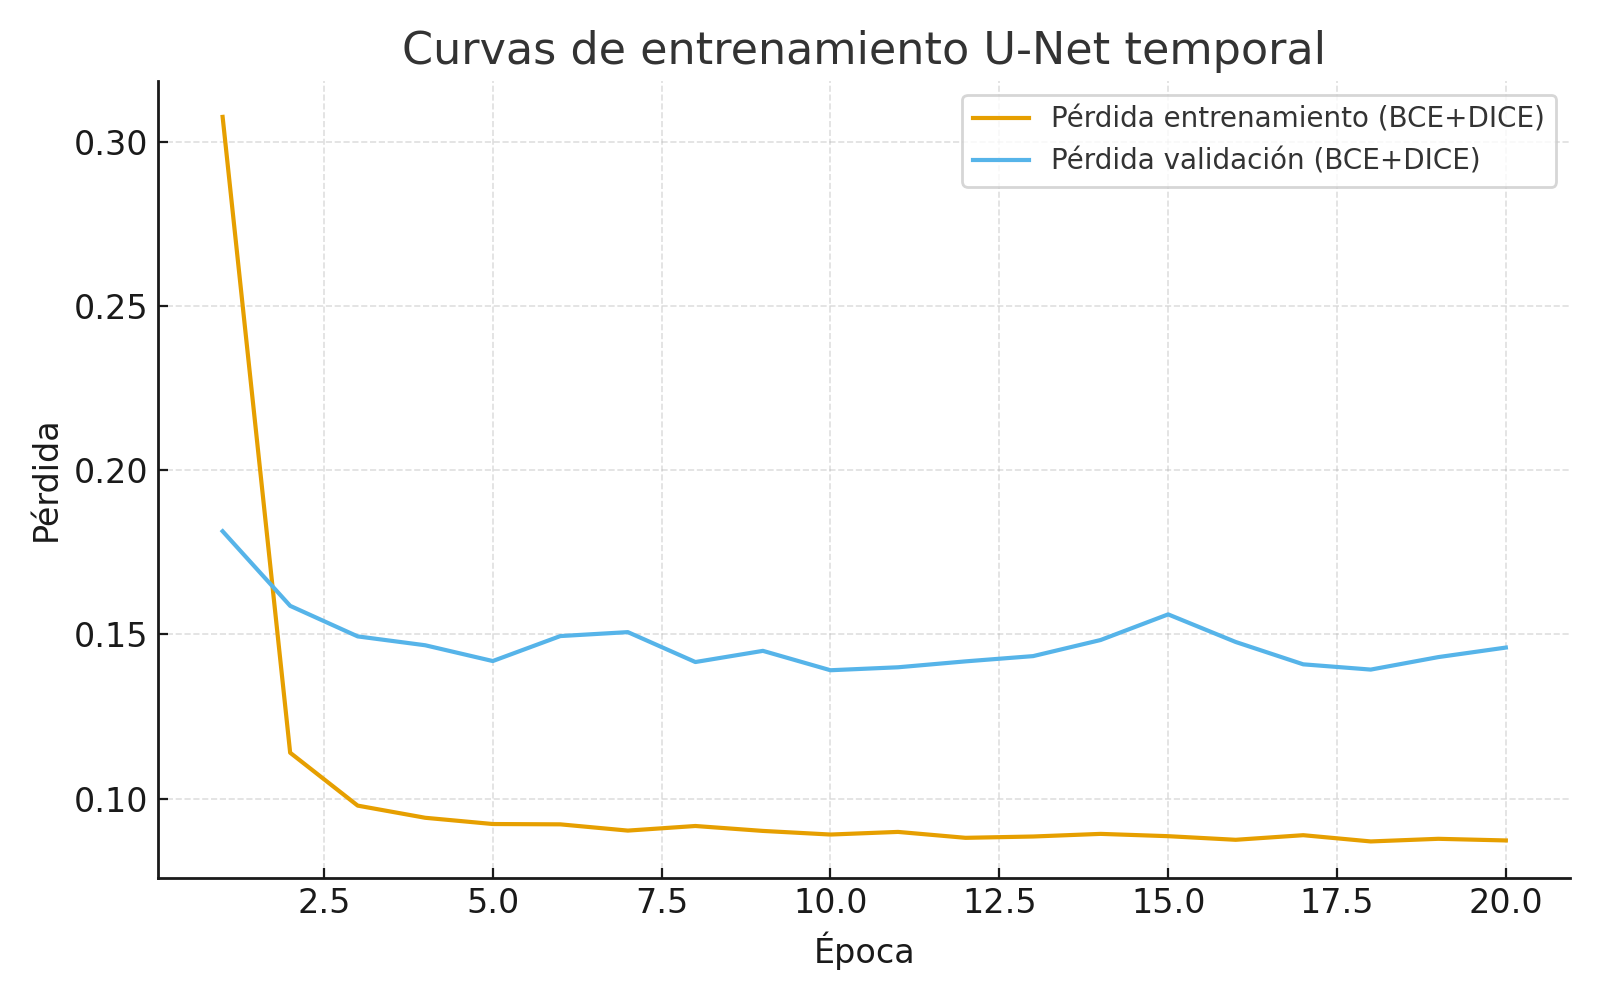
\includegraphics[scale=0.50]{Figures/curva_unet.png}
    \caption{Pronóstico usando CNN.}
    \label{fig:curva_unet}
\end{figure}


En síntesis, la U-Net temporal permite capturar patrones complejos de variación espacial y temporal, ofreciendo una herramienta flexible para el pronóstico de la cobertura de agua en la laguna del Salar de Llullaillaco.


%----------------------------------------------------------------------------------------
% 4.4 LIMITACIONES Y OBSERVACIONES
%----------------------------------------------------------------------------------------
\section{Limitaciones y observaciones}
A continuación se detallan las principales limitaciones,  supuestos y riesgo del trabajo realizado.

\subsection{Cobertura y calidad de datos}
\begin{itemize}
    \item Brechas temporales y SLC-off: la falla del Scan Line Corrector (SLC) en Landsat 7 (post mayo 2003) y la transición 2012–2013 generaron huecos relevantes. Se mitigó con una estrategia híbrida (interpolación en brechas cortas y promedio estacional en brechas largas), pero persiste incertidumbre residual en esos intervalos.
    \item Máscaras y umbrales: la detección de agua depende del umbral NDWI ($>0.2$). Cambios razonables en el umbral o en el tratamiento de nubes/sombras pueden modificar el área estimada (sensibilidad a parámetros).
    \item Validación in situ: no hubo verificación de campo, por lo que los umbrales y parámetros se justifican con literatura y coherencia interna; esto limita la cuantificación del sesgo absoluto.
\end{itemize}

\subsection{Supuestos estadísticos y diagnóstico de modelos}
\begin{itemize}
    \item Estacionariedad: ONI, SOI y MEI resultaron estacionarios por ADF, mientras que Área requirió diferenciación. El cumplimiento de estacionariedad es condición para SARIMA/VAR; desvíos locales pueden degradar el desempeño.
    \item Normalidad y heterocedasticidad de residuos: varios modelos (por ejemplo, ONI y MEI en SARIMA, y el VAR) muestran residuos no normales (colas pesadas) y, en casos, heterocedasticidad. Los intervalos de confianza deben interpretarse con cautela.
    \item Linealidad: Granger y VAR asumen relaciones lineales. Posibles no linealidades (o cambios de régimen) no modeladas pueden explicar parte del error, especialmente en picos del SOI.
    \item Métricas: el MAPE es poco informativo cuando hay valores cercanos a cero (índices ENSO). Se priorizaron RMSE/MAE y diagnóstico de residuos.
\end{itemize}

\subsection{Observaciones clave sobre resultados}
\begin{itemize}
    \item Serie Área: la diferenciación mejoró la robustez y redujo el error validando el preprocesamiento.
    \item ENSO: fuerte interdependencia entre ONI, SOI y MEI (Granger), con un rol central del SOI sobre Área. El VAR confirmó persistencia propia de cada índice y efectos cruzados coherentes con la física climática.
    \item SOI: aunque los residuos no presentan autocorrelación relevante, las métricas de error del modelo SARIMA fueron altas respecto de su escala, sugiriendo simplificación y/o modelos alternativos (por ejemplo, con heterocedasticidad).
    \item Segmentación con U-Net: el etiquetado automático mediante la red permitió generar una serie temporal estable sin necesidad de anotación manual, aunque con limitaciones en la cuantificación de métricas exhaustivas de segmentación.
\end{itemize}


\subsection{Riesgos y mitigaciones}
\begin{itemize}
    \item Dependencia de GEE y catálogos: fallos de disponibilidad pueden afectar la reproducibilidad. Mitigación: exportaciones imágenes.
    \item Sesgo por agregación espacial: el foco en la laguna central puede omitir dinámicas periféricas. Mitigación: probar la metodologia en otros sectores del salar.
     \item Complejidad computacional: el entrenamiento de modelos de segmentación y forecasting requiere recursos elevados. Mitigación: escalado progresivo, uso de subconjuntos y validación cruzada.
\end{itemize}



%----------------------------------------------------------------------------------------
% 4.5 CUMPLIMIENTO DE REQUERIMIENTOS
%----------------------------------------------------------------------------------------
\section{Cumplimiento de requerimientos}

A continuación se presenta el seguimiento del cumplimiento respecto de los requisitos definidos en la planificación. El estado se asigna con base en los desarrollos y resultados documentados (GEE/Colab, series temporales, SARIMA/VAR, visualizaciones y reportes).

\begin{table}[H]
\centering
\caption{Seguimiento de requisitos del proyecto}
\label{tab:requisitos_cumplimiento}
\resizebox{\textwidth}{!}{
\begin{tabular}{p{2cm} p{3cm} p{9cm}}
\toprule
Req. & Estado & Detalle \\
\midrule
\#1 & Cumple  & Descarga y procesamiento continuo desde GEE. \\
 & & Evidencia: pipelines en GEE con filtrado de nubes y exportación; brechas históricas (SLC-off, 2012–2013) cubiertas con imputación. \\
\#2 & Cumple & Modelos IA predicen en menos de 24 h. \\
 & & Evidencia: SARIMA/VAR ejecutan en horas sobre dataset mensual; validado en Colab. \\
\#3 & Cumple & Visualización de mapas y series temporales. \\
 & & Evidencia: mapas de ocurrencia e índices ACF/PACF y predicciones incluidos en resultados. \\
\#4 & Cumple & Cálculo de NDWI en menos de 30 min por lote. \\
 & & Evidencia: en lotes representativos se cumple; falta protocolo formal de benchmark. \\
\#5 & Cumple & Precisión mínima 80\% en disponibilidad de agua. \\
 & & Evidencia: métricas RMSE/MAE favorables para Área/Área\_diff; falta métrica categórica y validación externa. \\
\#6 & Cumple & Compatibilidad con GeoTIFF y Shapefile. \\
 & & Evidencia: recortes vectoriales y exportaciones desde GEE. \\
\#7 & Cumple & Documentación técnica detallada. \\
 & & Evidencia: metodología y apéndices en desarrollo; resta manual de usuario. \\
\#8 & Pendiente & Pruebas con Sentinel-2. \\
 & & Evidencia: validación cruzada multi-sensor planificada; aún no ejecutada. \\
\#9 & Cumple & Cumplimiento de políticas GEE académicas. \\
 & & Evidencia: uso no comercial, citación de colecciones, límites de cuota. \\
\#10 & Cumple & Reportes claros para usuarios. \\
 & & Evidencia: resumen ejecutivo y tablas listos; falta consolidar executive brief y anexo metodológico. \\
\bottomrule
\end{tabular}
}
\end{table}

Los requisitos operativos de datos, modelado y visualización se encuentran cumplidos o muy avanzados. Permanecen en progreso las pruebas con Sentinel-2 (Req.\,\#8).



% Chapter Template

\chapter{Conclusiones} % Main chapter title

\label{Chapter5} % Change X to a consecutive number; for referencing this chapter elsewhere, use \ref{ChapterX}
Este capítulo presenta las conclusiones generales del trabajo, resumiendo los aportes más relevantes obtenidos y el grado de cumplimiento de los objetivos planteados. Asimismo, se incluyen observaciones sobre la planificación y los riesgos, y se señalan posibles líneas de desarrollo futuro. 

%----------------------------------------------------------------------------------------
%	SECTION 1
%----------------------------------------------------------------------------------------

\section{Conclusiones generales }
El trabajo permitió caracterizar la dinámica temporal de la superficie de agua en el Salar de Llullaillaco y su relación con los principales índices climáticos asociados al ENSO. A partir de la construcción de un cubo temporal mensual continuo y de la aplicación de metodologías estadísticas y de aprendizaje profundo, se alcanzaron hallazgos relevantes sobre la influencia climática regional en la hidrología altoandina. 

Entre los principales resultados se destaca que el SOI emergió como el índice con mayor capacidad explicativa sobre la superficie de agua, confirmado por los modelos VAR y la prueba de causalidad de Granger. La integración de SARIMA y VAR permitió capturar la estacionalidad y las interdependencias multivariadas, mientras que la segmentación automática con U-Net facilitó la generación de series homogéneas sin necesidad de etiquetado manual. En síntesis, se validó la hipótesis de que la variabilidad climática global, en particular el ENSO, constituye un factor determinante en la dinámica hídrica del salar.


A partir de la planificación inicial y las pruebas desarrolladas, se alcanzaron los siguientes logros y hallazgos principales:

\begin{itemize}
    \item Se construyó un cubo temporal mensual continuo de la superficie de agua (1984--2022), combinando interpolación e imputación estacional para cubrir vacíos y asegurar homogeneidad en la serie.
    \item La segmentación con U-Net, entrenada mediante el esquema \emph{knowledge distillation}, permitió generar máscaras mensuales de agua de manera automática, evitando la necesidad de etiquetado manual y aportando consistencia espacial y temporal.
    \item A partir de estas máscaras se derivó la serie de Área, que mostró estacionariedad solo tras diferenciación, mientras que las series climáticas ONI, SOI y MEI fueron estacionarias desde el inicio.
    \item Los modelos SARIMA mostraron buen ajuste, destacándose la serie diferenciada de Área con residuos consistentes con ruido blanco; el SOI resultó más complejo de modelar por su alta variabilidad.
    \item El modelo VAR(3) capturó interdependencias multivariadas entre ONI, SOI y MEI, confirmando la influencia significativa del SOI sobre el Área, resultado reforzado por la prueba de causalidad de Granger y las respuestas al impulso.
    \item Se realizaron pronósticos mediante \emph{rolling forecast} con SARIMA y VAR, validando la capacidad predictiva de ambas metodologías y evidenciando limitaciones en la captura de picos extremos.
    \item Se cumplió la mayoría de los requisitos planteados en la planificación: construcción de series homogéneas, modelado SARIMA/VAR, segmentación automática con U-Net, validación de resultados y visualización. Permanecen en progreso las métricas de precisión categórica y las pruebas cruzadas con Sentinel-2.
    \item Los riesgos identificados (brechas satelitales, errores en índices) no se materializaron de manera crítica; las medidas de mitigación fueron efectivas, aunque la alta variabilidad del SOI y la necesidad de preprocesamiento riguroso se mantuvieron como los principales desafíos.
\end{itemize}


En síntesis, el trabajo permitió validar la hipótesis inicial: la variabilidad climática global asociada al ENSO, en especial la expresada por el SOI, constituye un factor determinante en la dinámica hídrica del Salar de Llullaillaco.

%----------------------------------------------------------------------------------------
%	SECTION 2
%----------------------------------------------------------------------------------------

\section{Próximos pasos}

El trabajo abre la posibilidad de ampliar la metodología hacia nuevas aplicaciones y mejoras técnicas. Entre ellas, la extensión a otros salares de la Puna y el altiplano para evaluar la consistencia regional, la incorporación de sensores adicionales como Sentinel-2, y la exploración de modelos de inteligencia artificial avanzados (LSTM, transformers) capaces de capturar relaciones no lineales y patrones complejos. 

Asimismo, resulta prioritario profundizar el análisis de incertidumbre mediante modelos que contemplen heterocedasticidad y distribuciones no gaussianas, e integrar variables hidrometeorológicas locales (precipitación, temperatura, evapotranspiración) que complementen los indicadores climáticos globales. Estos pasos permitirán consolidar la base metodológica y avanzar hacia sistemas predictivos robustos que respalden la gestión ambiental en ecosistemas de altura.


%----------------------------------------------------------------------------------------
% Apéndices
%----------------------------------------------------------------------------------------

\appendix

% Incluir apéndices desde archivos separados si es necesario
% Appendix A

\chapter{Figuras} % Main appendix title

\label{AppendixA} % For referencing this appendix elsewhere, use \ref{AppendixA}


\begin{figure}[ht]
        \centering
        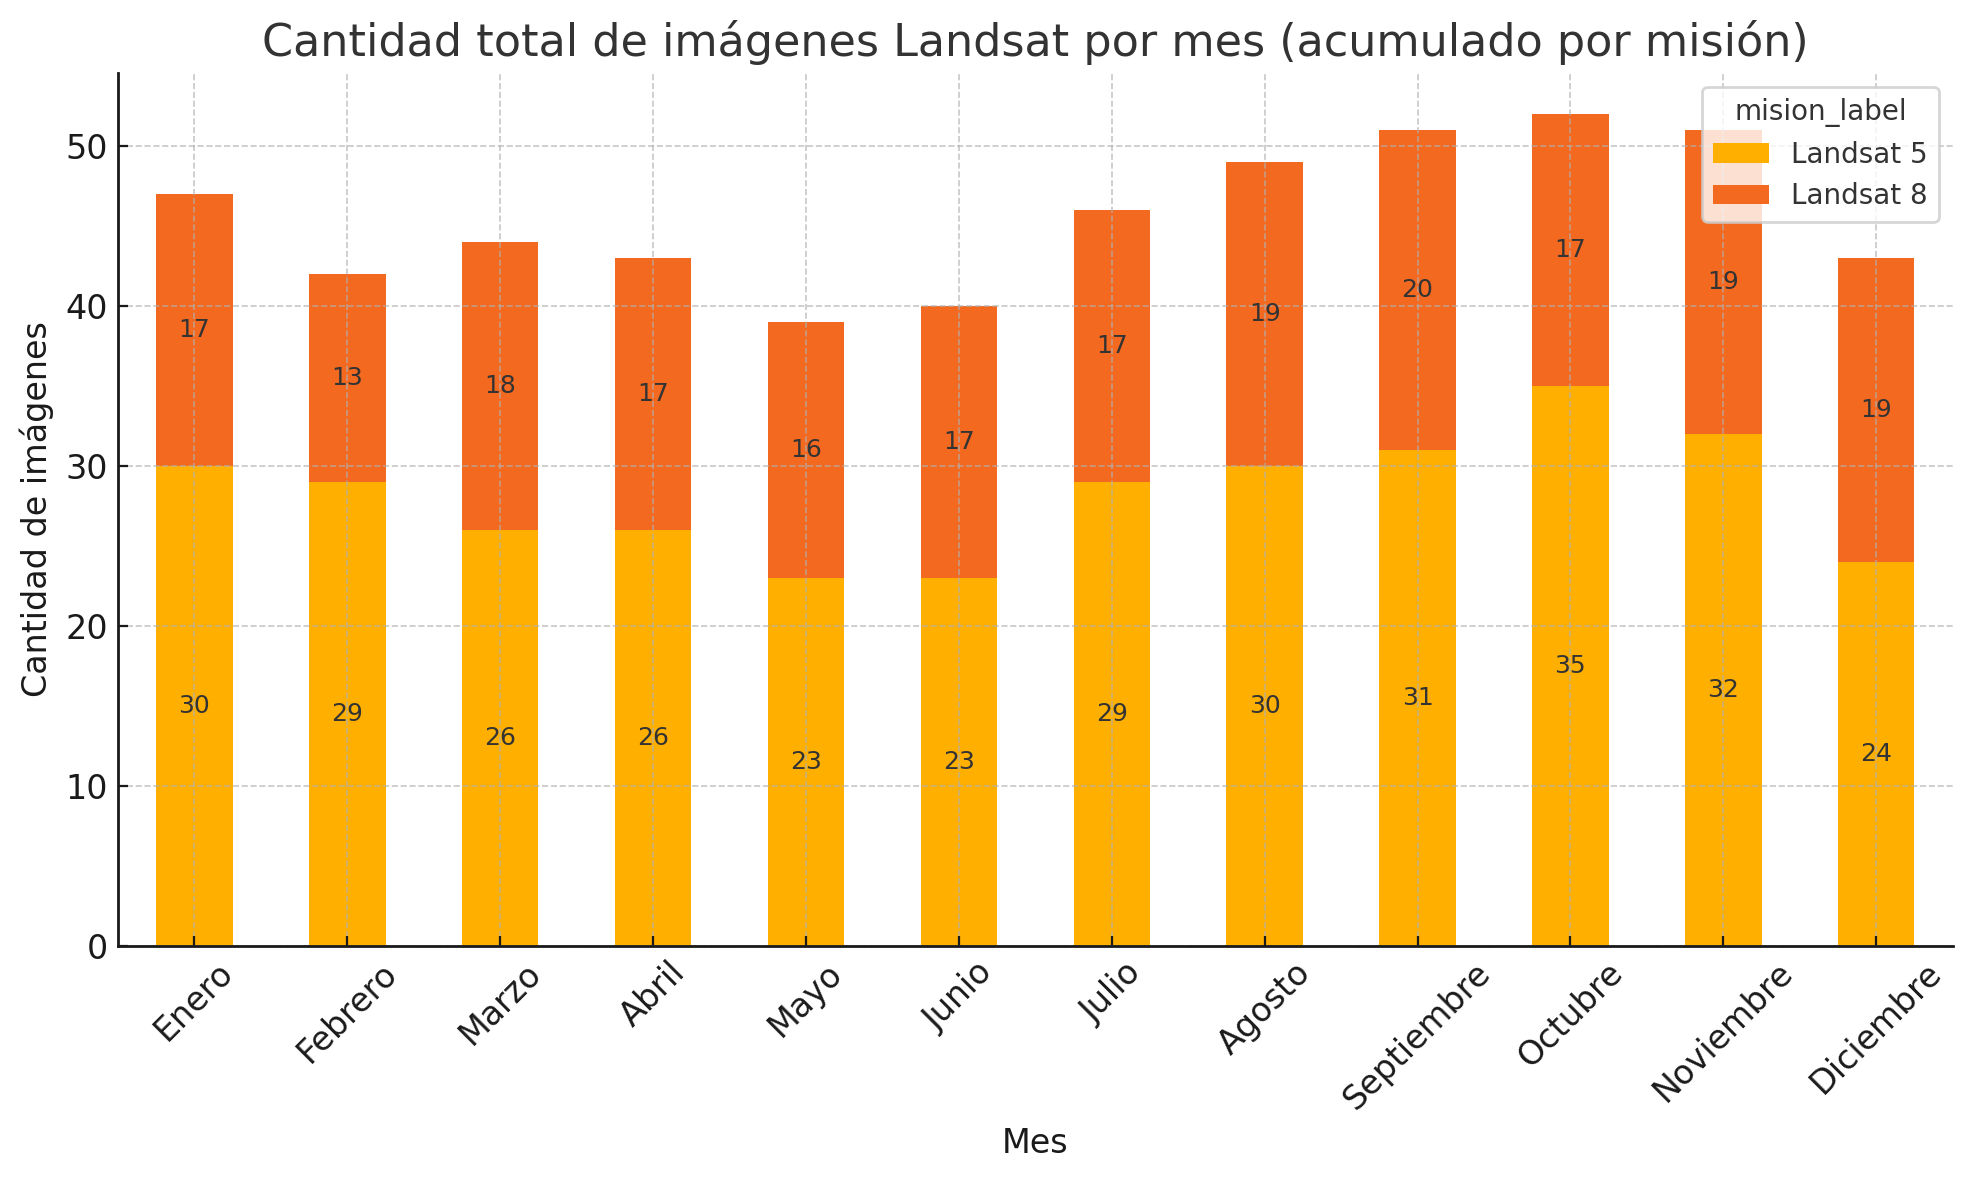
\includegraphics[scale=.4]
        {Figures/fig12.png}
        \caption{Cantidad de imágenes por mes y misión.}
        \label{fig:cant_imagenes}
\end{figure}

\begin{figure}[htpb]
    \centering
    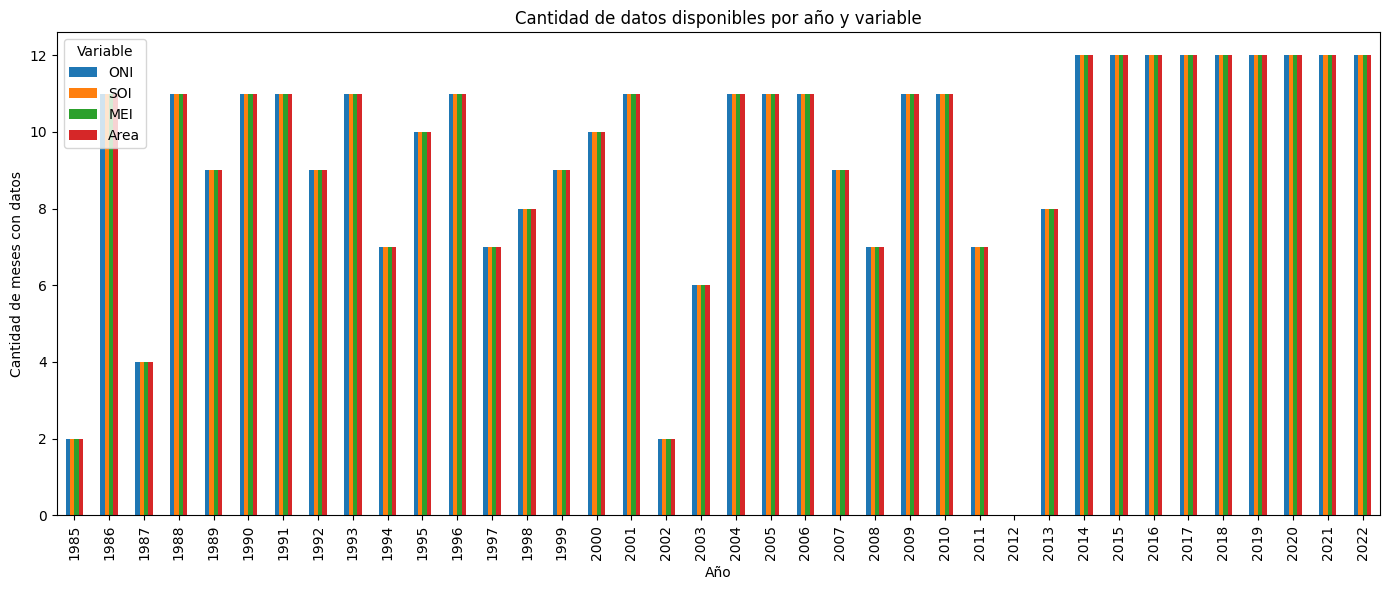
\includegraphics[scale=.40]{Figures/conteo_series.png}
    \caption{Cantidad de meses con datos disponibles por año y variable (ONI, SOI, MEI, Área).}
    \label{fig:conteo_datos}
\end{figure}

\begin{figure}[ht]
        \centering
        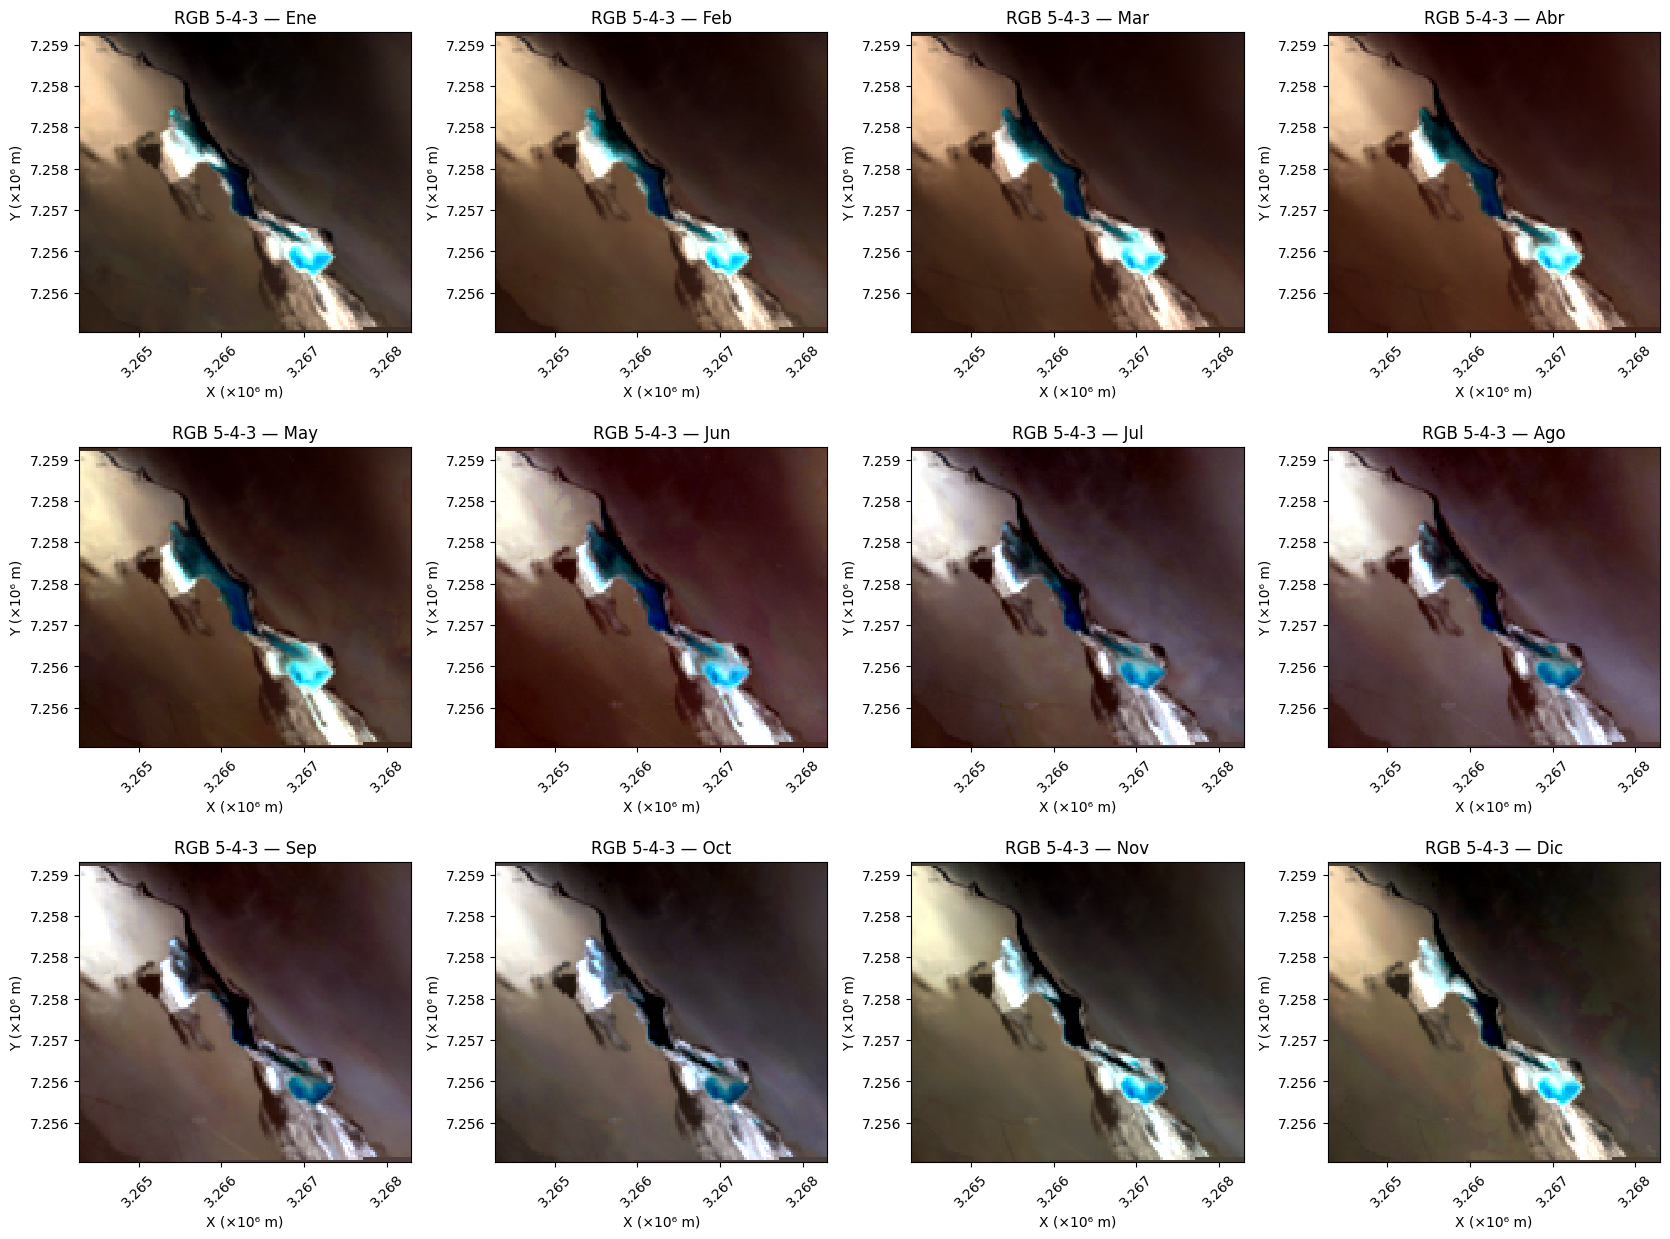
\includegraphics[scale=.30]
        {Figures/mensualimg_.png}
        \caption{Imágenes medianas mensuales de la serie histórica.}
        \label{fig:img_mens}
\end{figure}


\begin{figure}[ht]
        \centering
        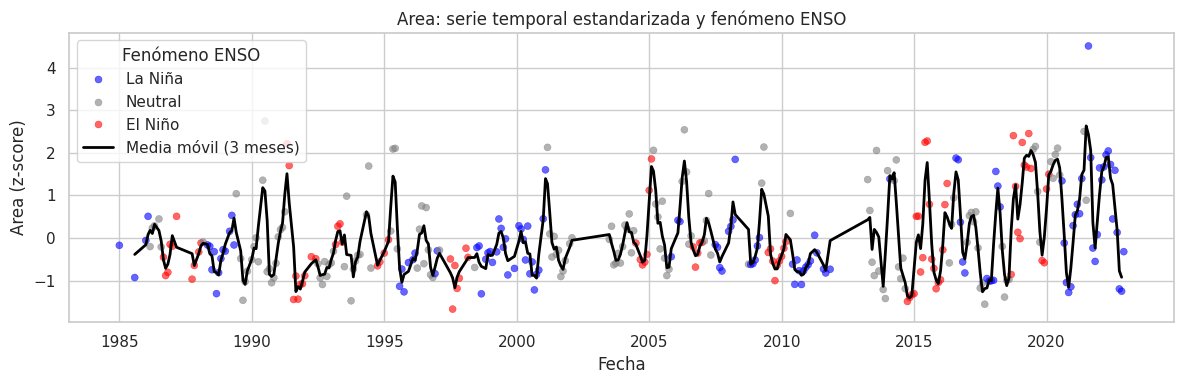
\includegraphics[scale=.45]
        {Figures/fig16_ts_area.png}
        \caption{Registro histórico de la variable Área (1984-2022).}
        \label{fig:indice_area}
\end{figure}


\begin{figure}[ht]
        \centering
        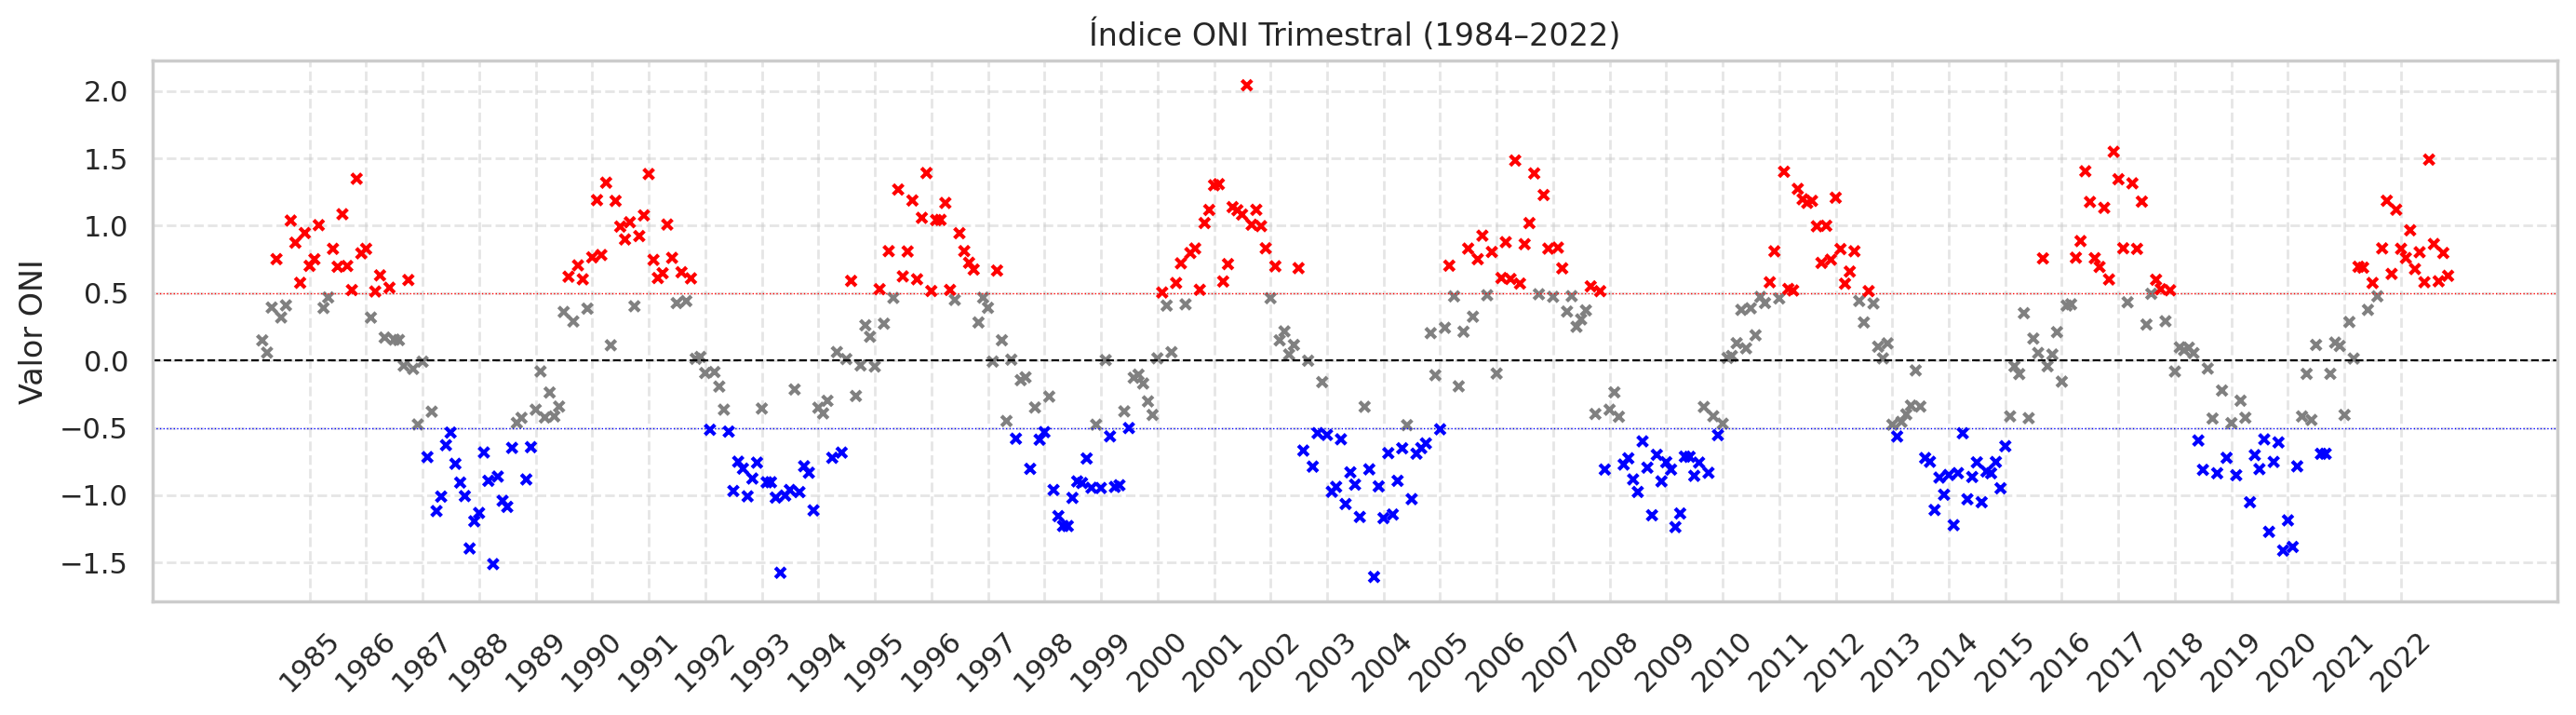
\includegraphics[scale=.38]
        {Figures/fig13_oni.png}
        \caption{Índice ONI (1984-2022).}
        \label{fig:indice_oni}
\end{figure}

\begin{figure}[ht]
        \centering
        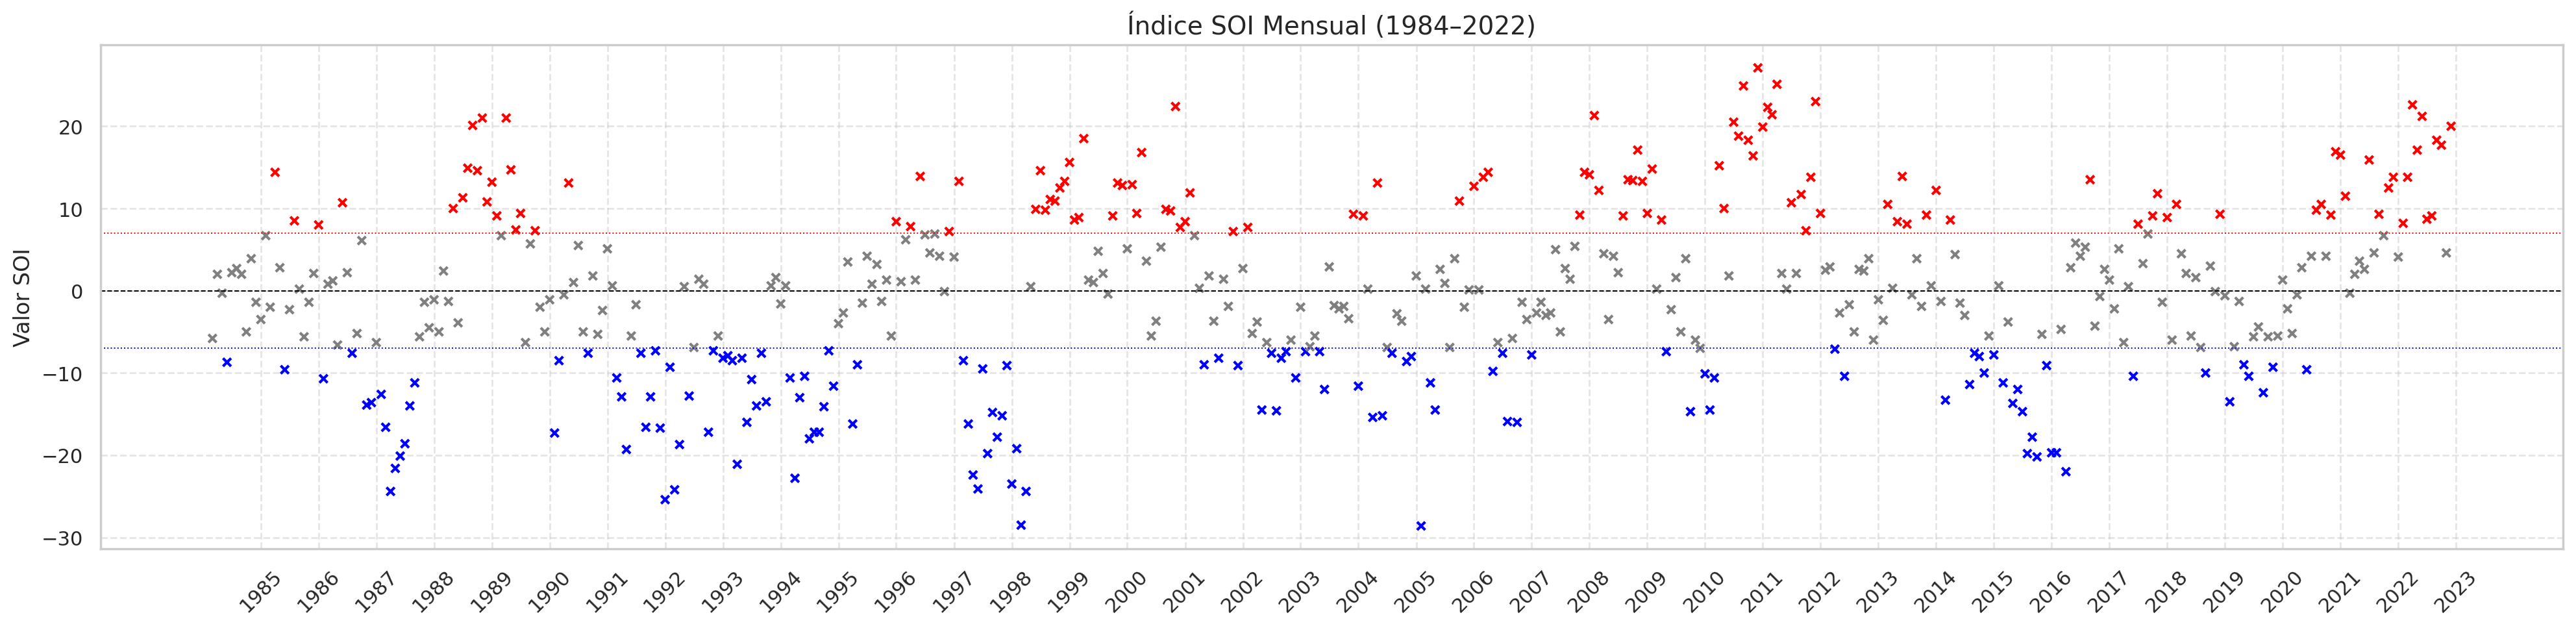
\includegraphics[scale=.26]
        {Figures/fig14_soi.png}
        \caption{Índice SOI (1984-2022).}
        \label{fig:indice_soi}
\end{figure}

\begin{figure}[ht]
        \centering
        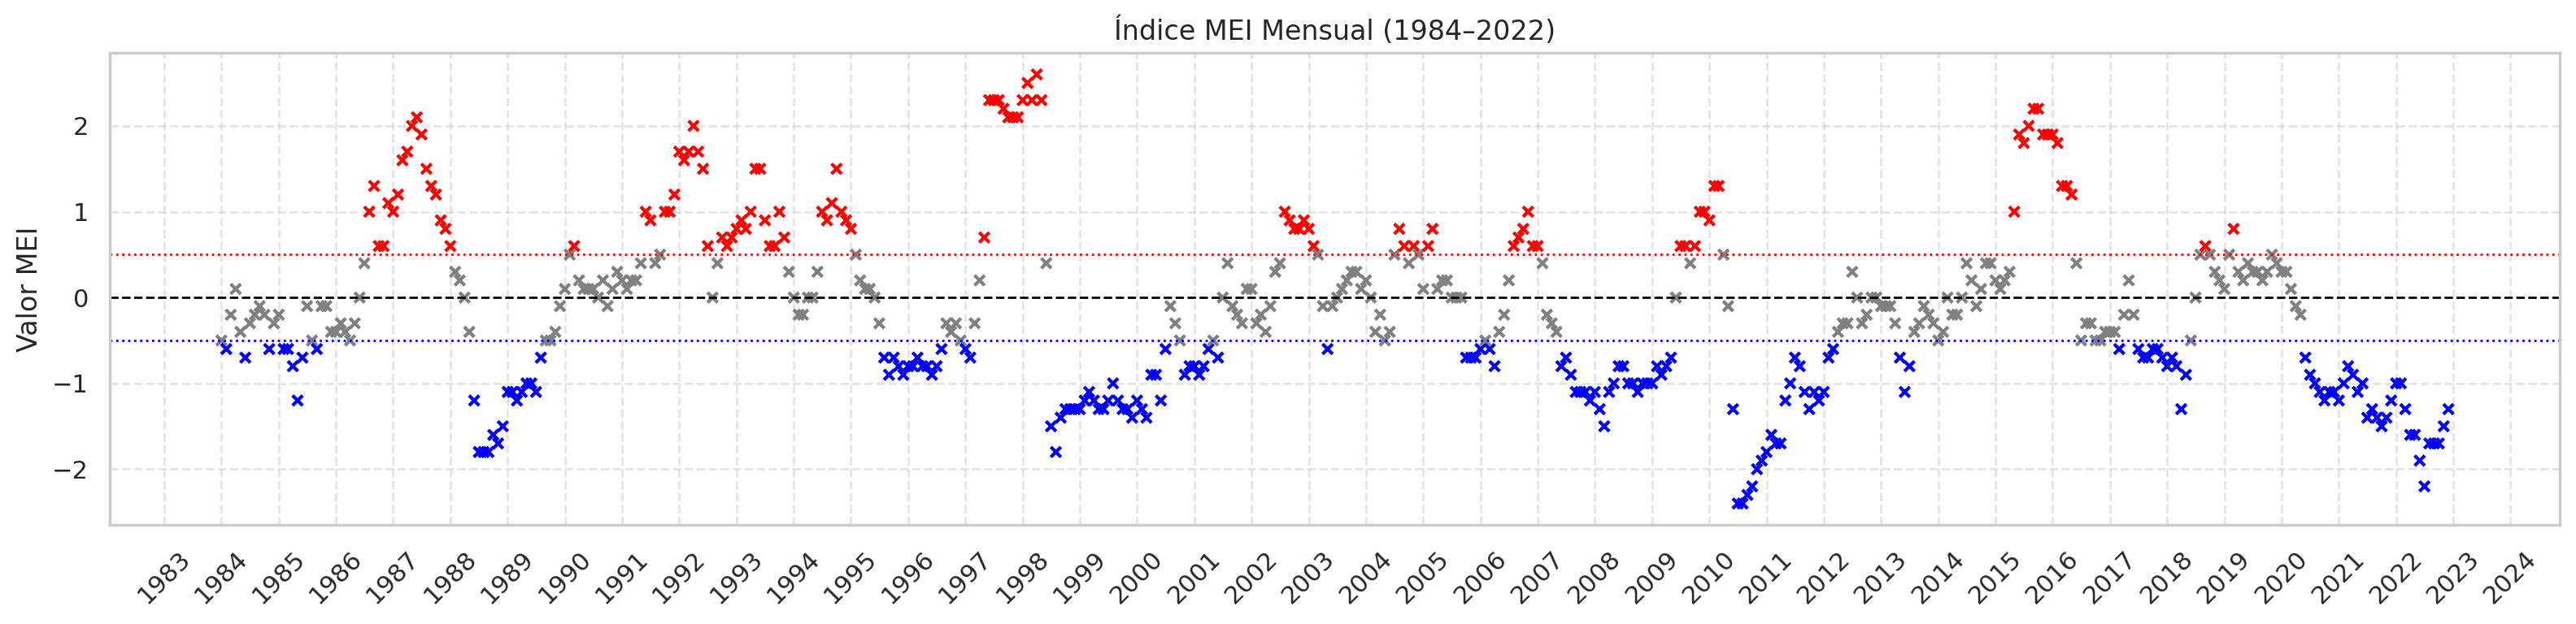
\includegraphics[scale=.32]
        {Figures/fig15_mei.png}
        \caption{Índice MEI (1984-2022).}
        \label{fig:indice_mei}
\end{figure}

\begin{figure}[ht]
        \centering
        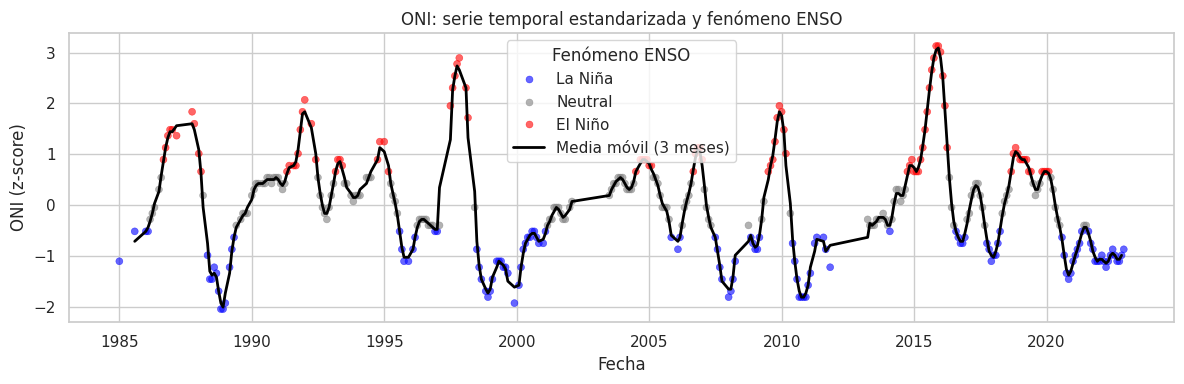
\includegraphics[scale=.45]
        {Figures/fig17_ts_oni.png}
        \caption{Índice ONI (1984-2022).}
        \label{fig:indice_oni_ts}
\end{figure}

\begin{figure}[ht]
        \centering
        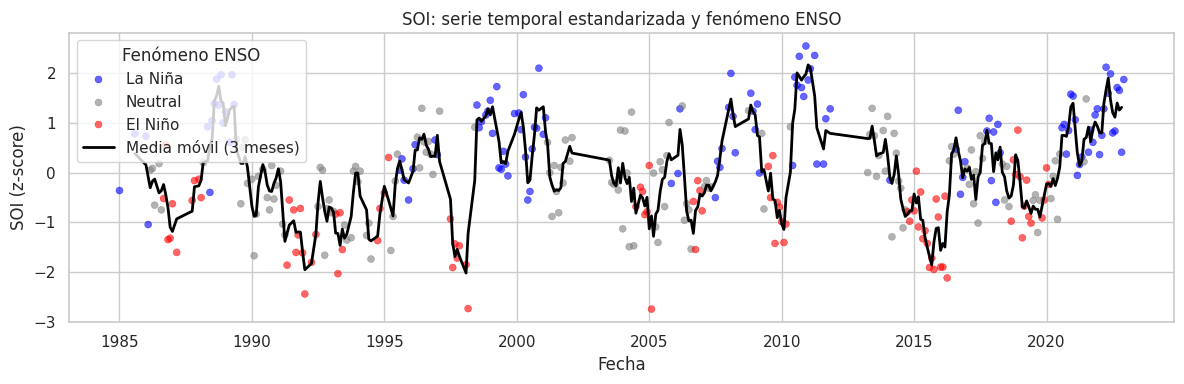
\includegraphics[scale=.45]
        {Figures/fig18_ts_soi.png}
        \caption{Índice SOI (1984-2022).}
        \label{fig:indice_soi_ts}
\end{figure}

\begin{figure}[ht]
        \centering
        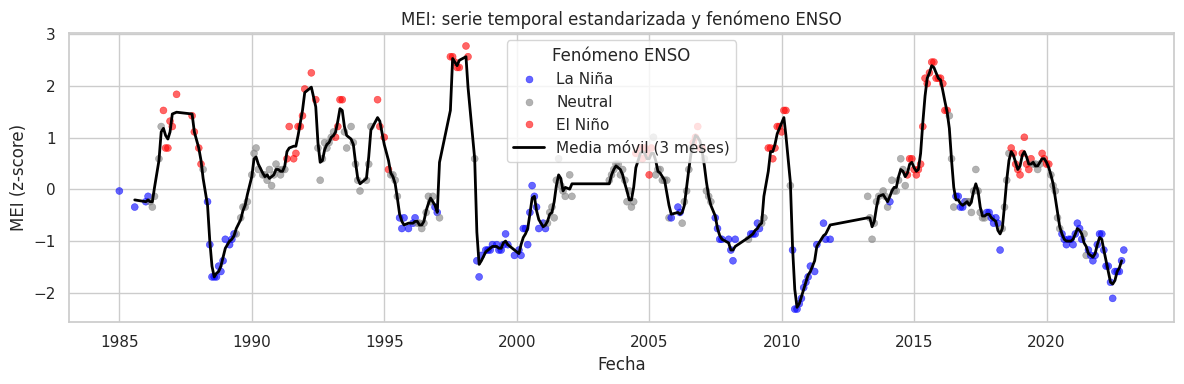
\includegraphics[scale=.45]
        {Figures/fig19_ts_mei.png}
        \caption{Índice MEI (1984-2022).}
        \label{fig:indice_mei_ts}
\end{figure}
\newpage


\begin{figure}[H]
    \centering
    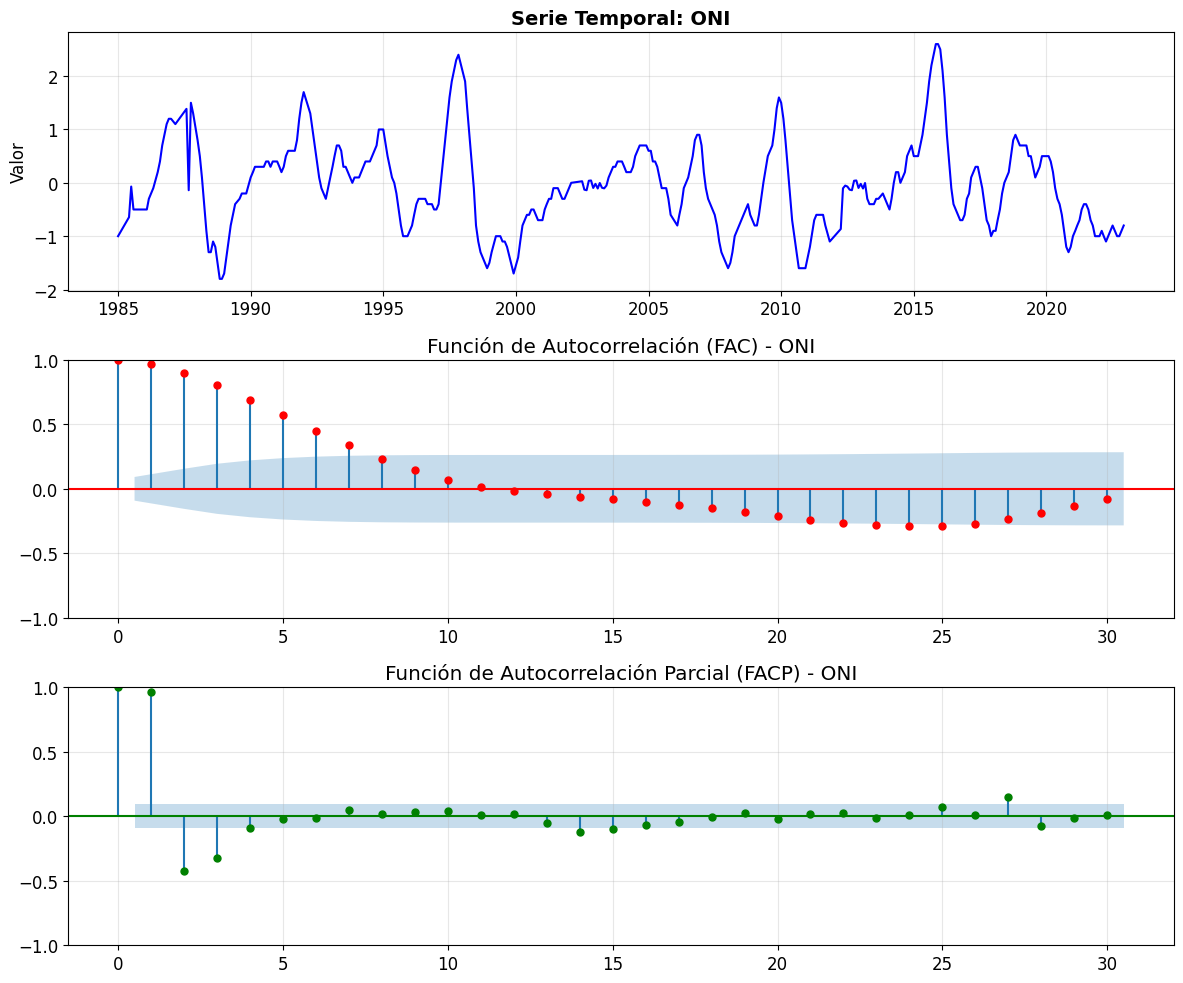
\includegraphics[scale=.42]{Figures/facp_ONI.png}
    %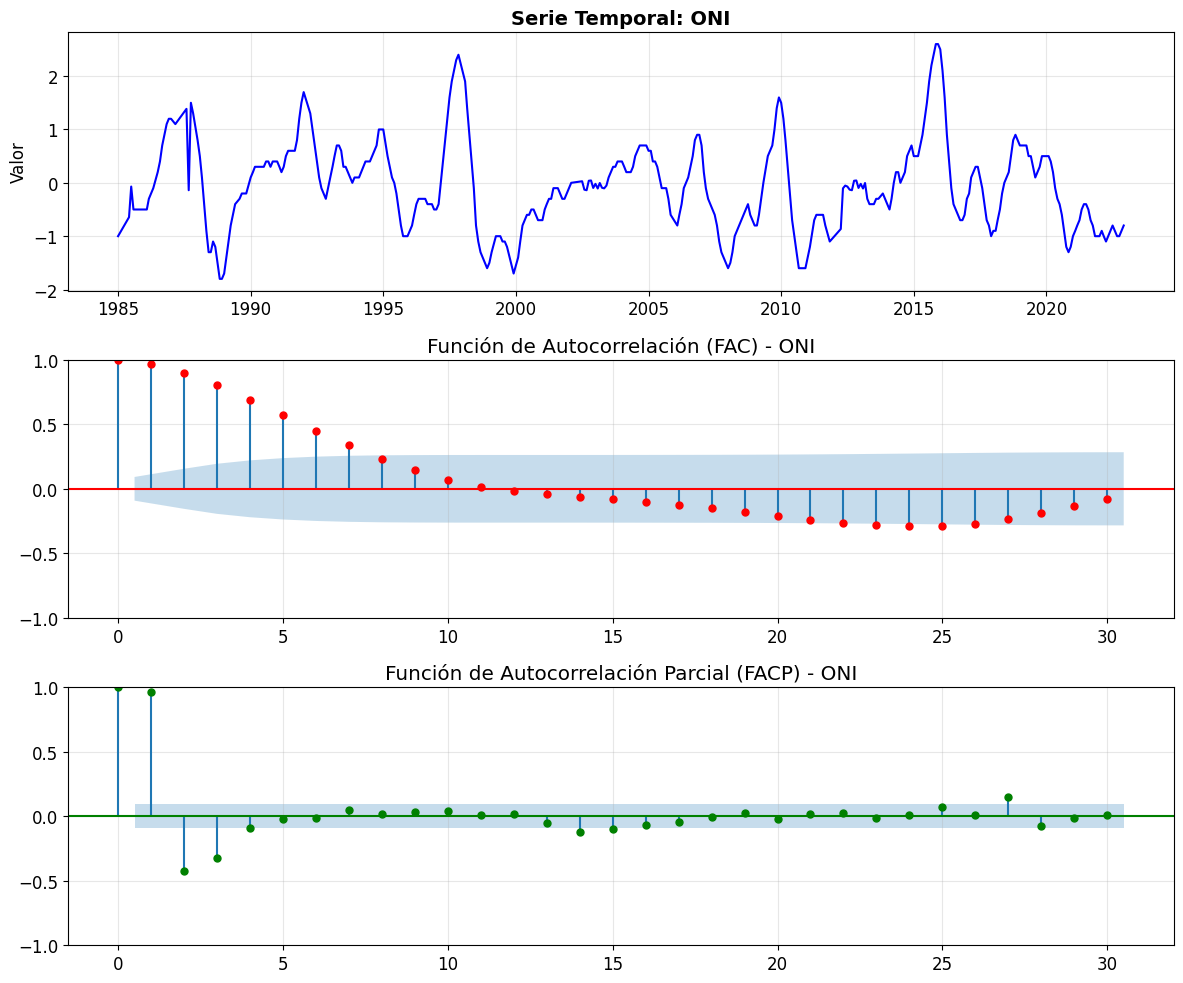
\includegraphics[width=0.7\textwidth]{Figures/facp_ONI.png}
    \caption{Funciones ACF y PACF de la serie ONI.}
    \label{fig:facp_oni}
\end{figure}

\begin{figure}[H]
    \centering
    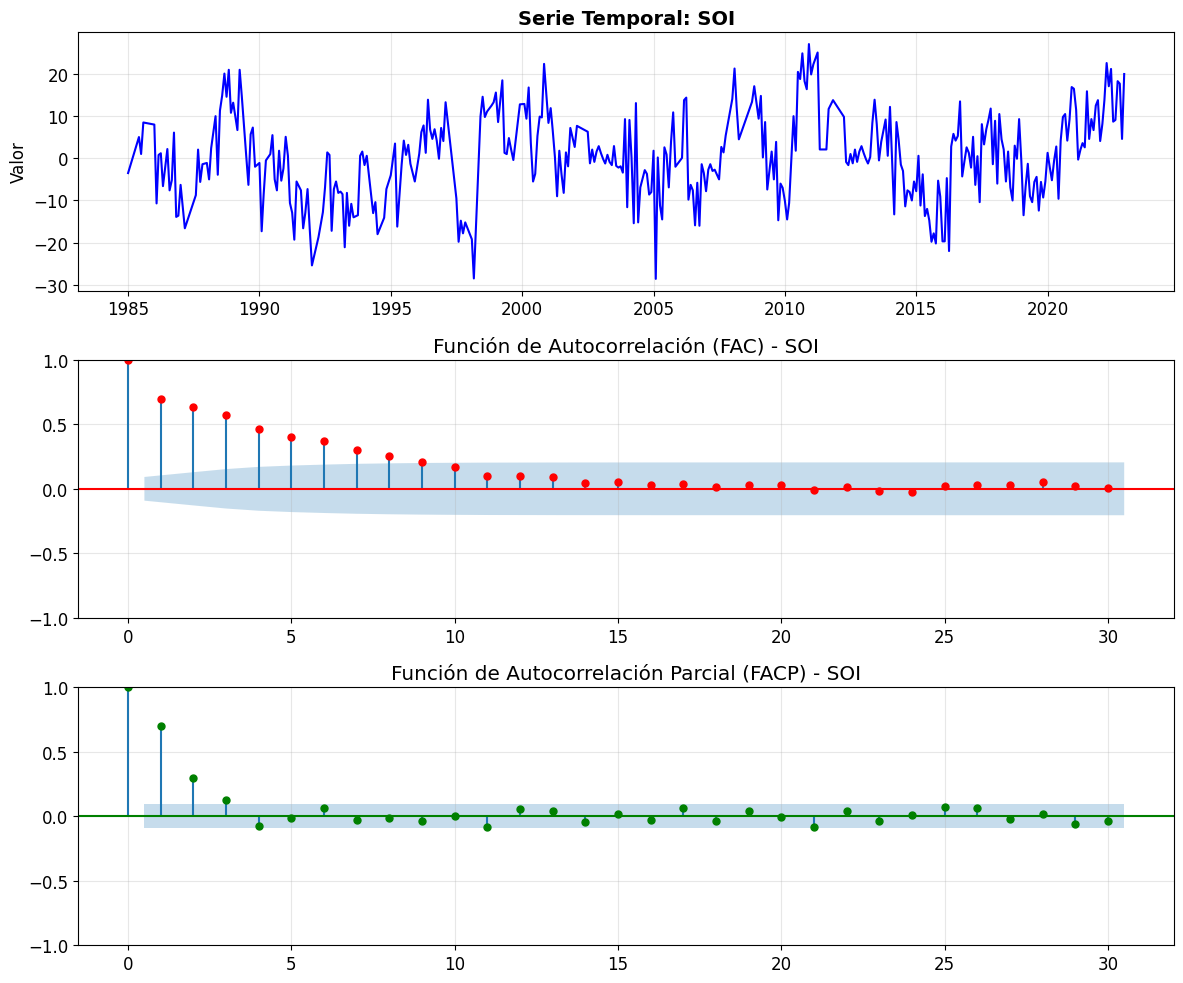
\includegraphics[scale=.42]{Figures/facp_SOI.png}
    \caption{Funciones ACF y PACF de la serie SOI.}
    \label{fig:facp_soi}
\end{figure}

\begin{figure}[H]
    \centering
    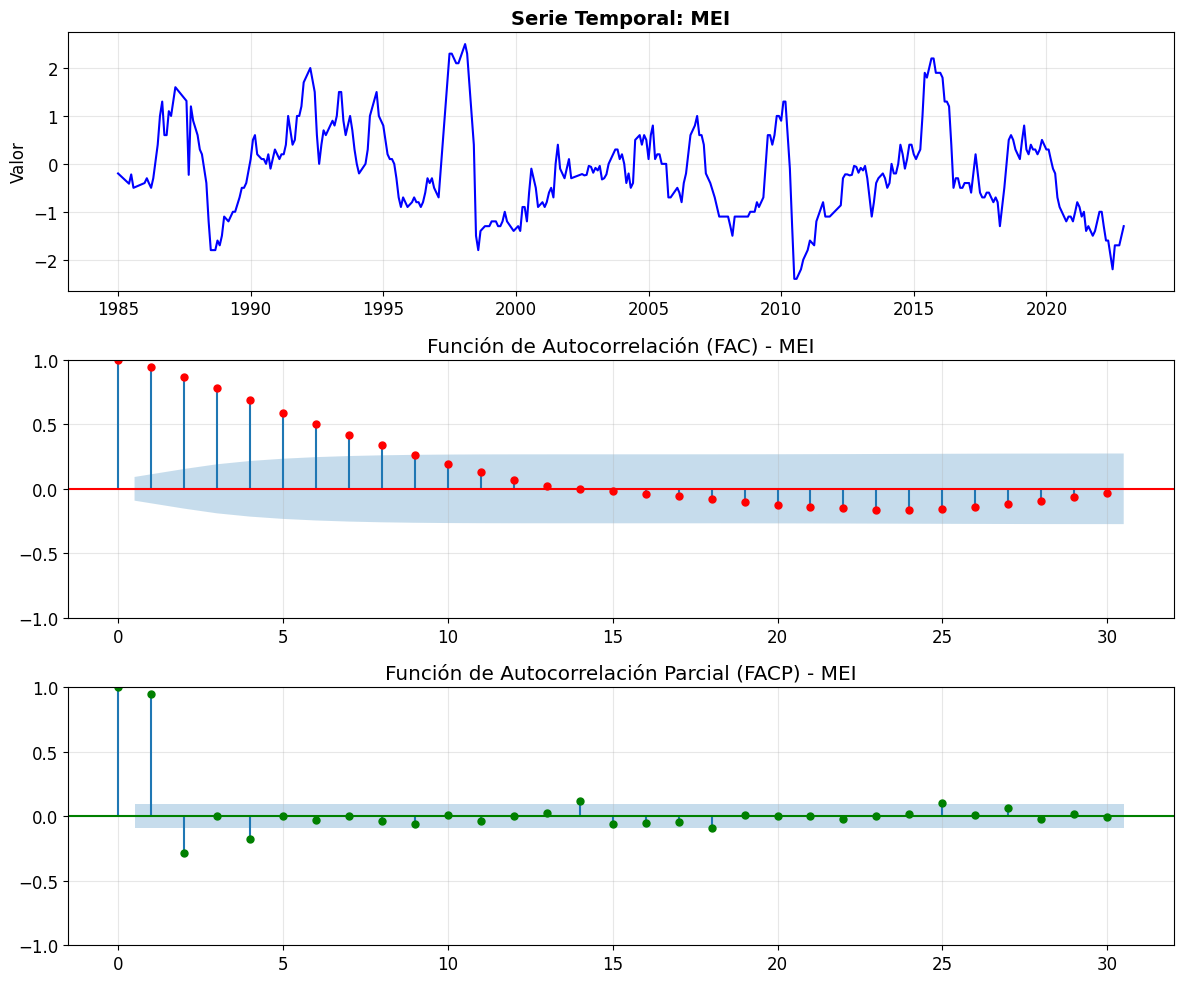
\includegraphics[scale=.42]{Figures/facp_MEI.png}
    \caption{Funciones ACF y PACF de la serie MEI.}
    \label{fig:facp_mei}
\end{figure}

\begin{figure}[H]
    \centering
    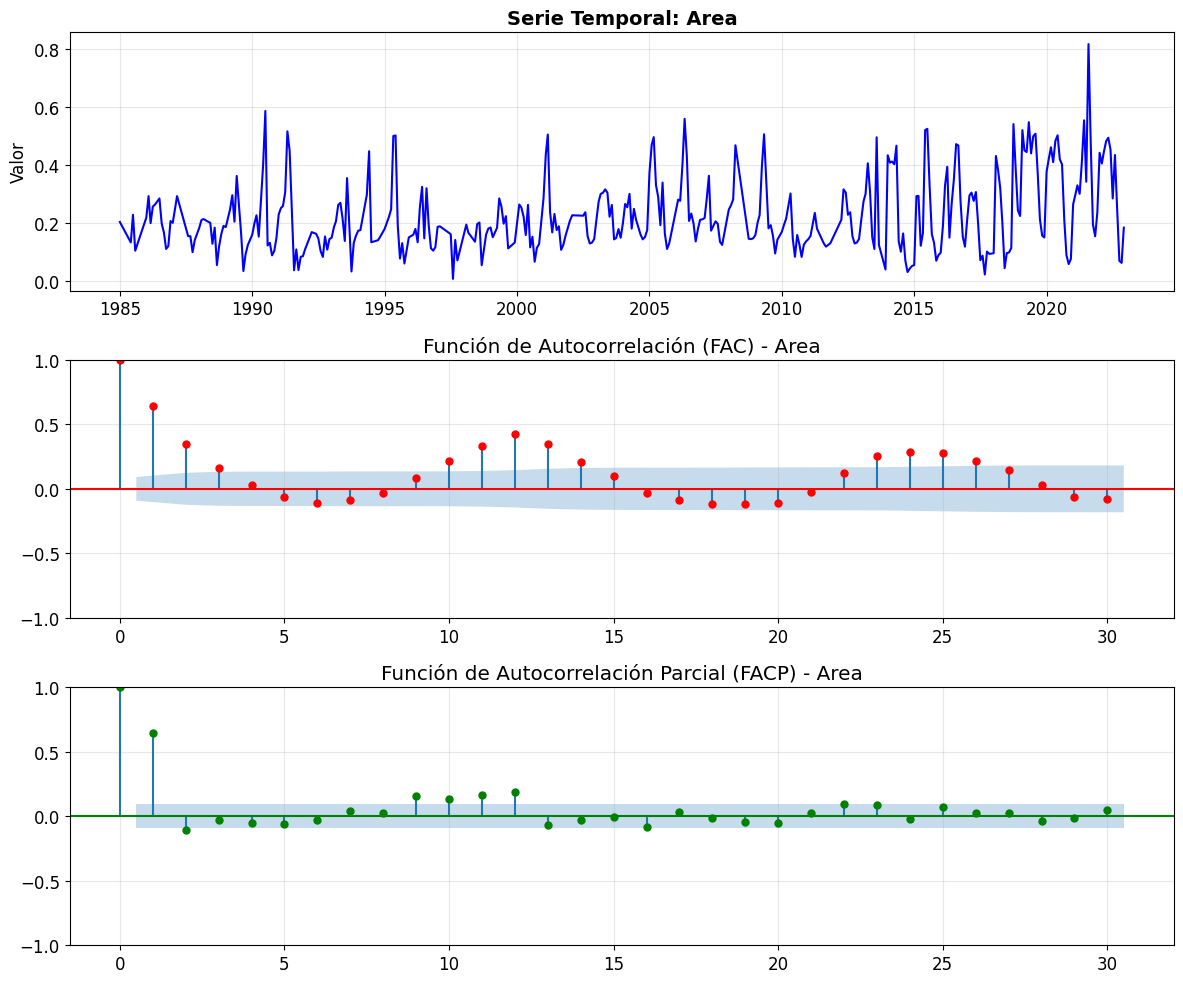
\includegraphics[scale=.42]{Figures/facp_Area.png}
    \caption{Funciones ACF y PACF de la serie Área (superficie de agua).}
    \label{fig:facp_area}
\end{figure}


\begin{figure}[H]\centering
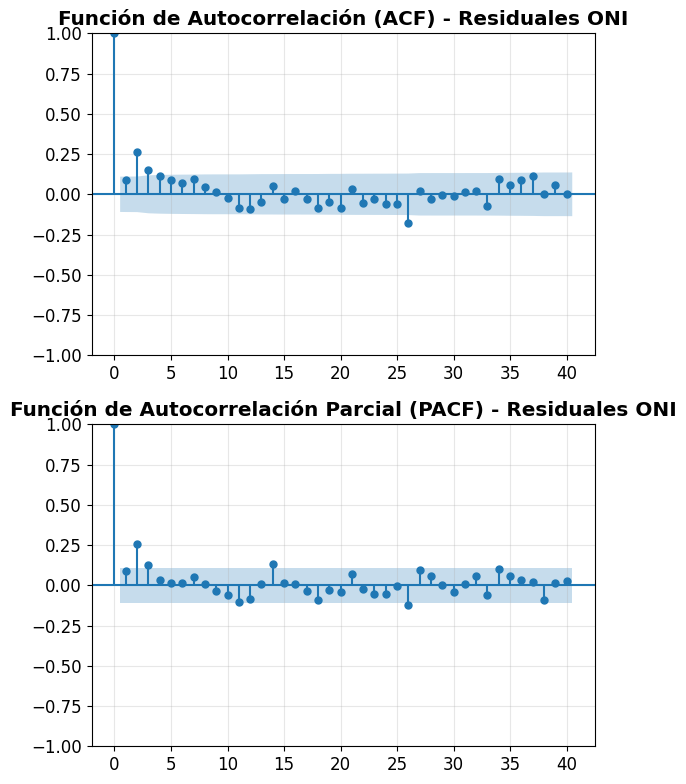
\includegraphics[scale=.52]{Figures/acf_pacf_res_oni.png}
\caption{ONI: ACF y PACF de los residuos.}
\label{fig:acf_pacf_res_oni}
\end{figure}

\begin{figure}[H]\centering
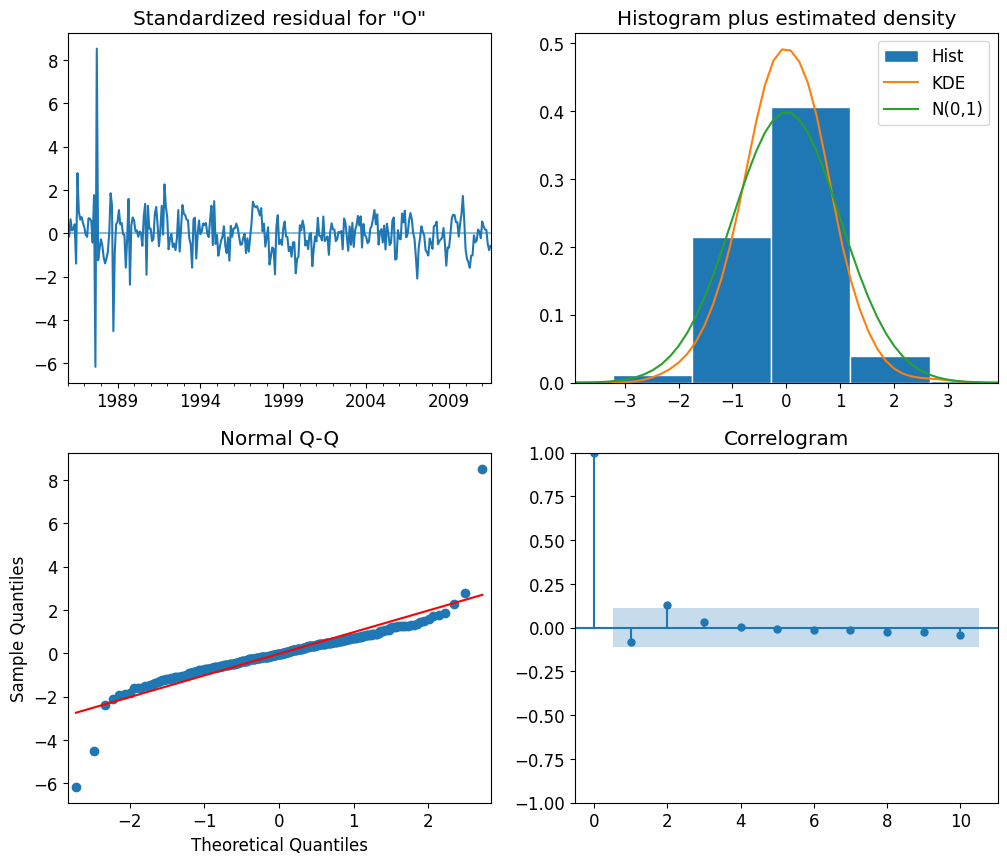
\includegraphics[scale=.52]{Figures/res_std_oni.png}
\caption{ONI: diagnóstico estándar de residuos (histograma, densidad, Q--Q, correlograma).}
\label{fig:std_oni}
\end{figure}

\begin{figure}[H]\centering
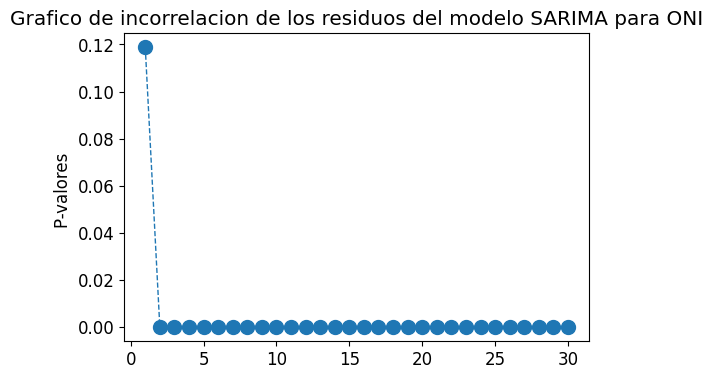
\includegraphics[scale=.52]{Figures/inco_oni.png}
\caption{ONI: gráfico de incorrelación (p--valores Ljung--Box por lag).}
\label{fig:inco_oni}
\end{figure}


\begin{figure}[H]\centering
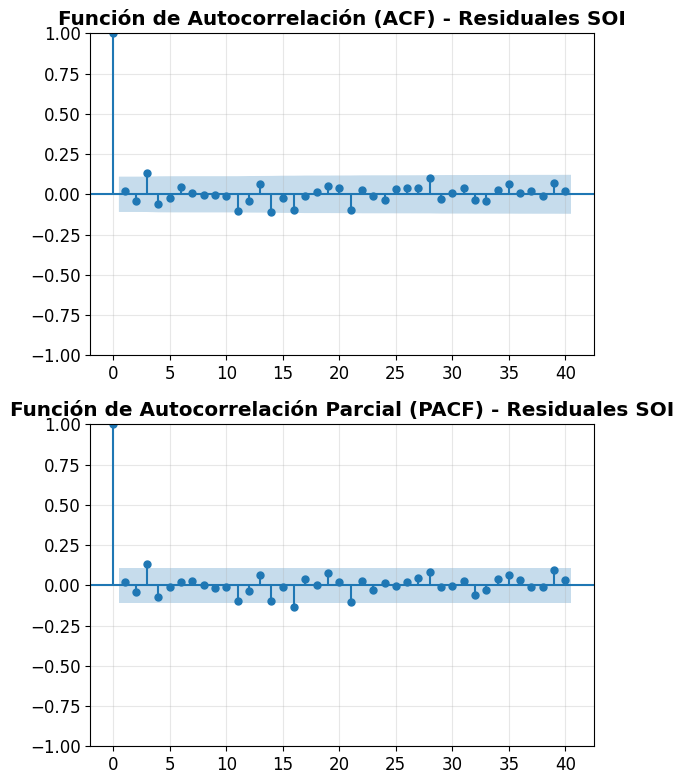
\includegraphics[scale=.52]{Figures/acp_pacf_res_soi.png}
\caption{SOI: ACF y PACF de los residuos.}
\label{fig:acf_pacf_res_soi}
\end{figure}

\begin{figure}[H]\centering
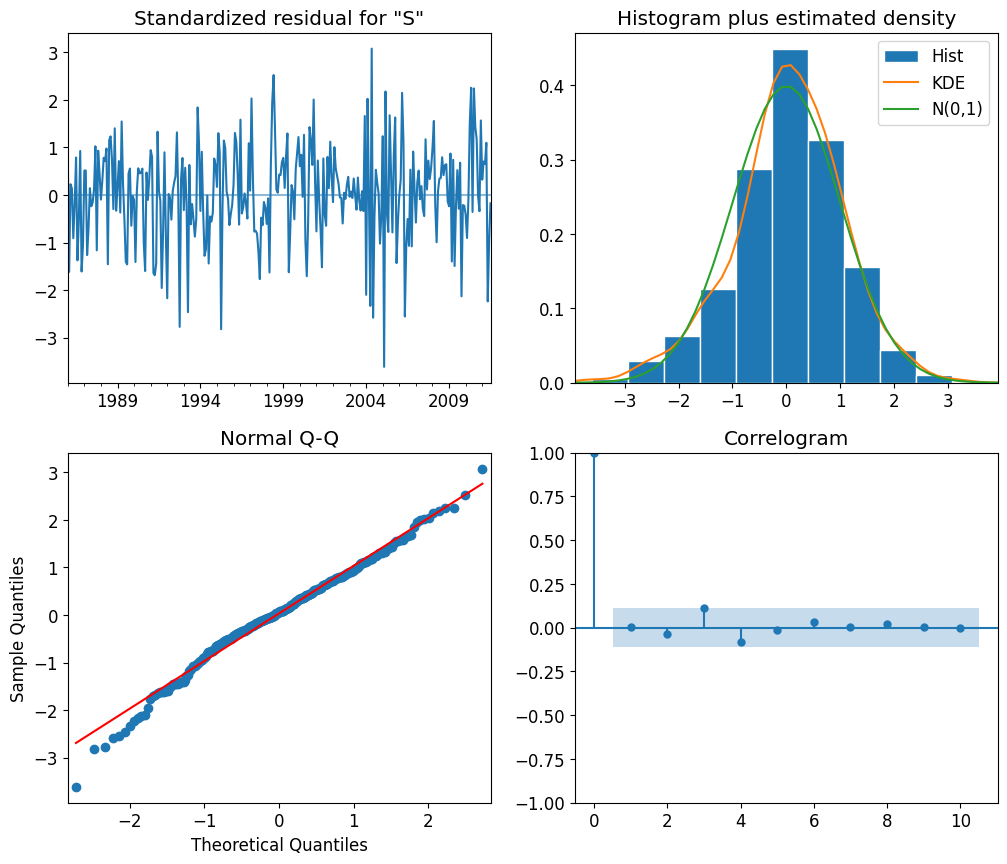
\includegraphics[scale=.52]{Figures/res_std_soi.png}
\caption{SOI: diagnóstico estándar de residuos (histograma, densidad, Q--Q, correlograma).}
\label{fig:std_soi}
\end{figure}

\begin{figure}[H]\centering
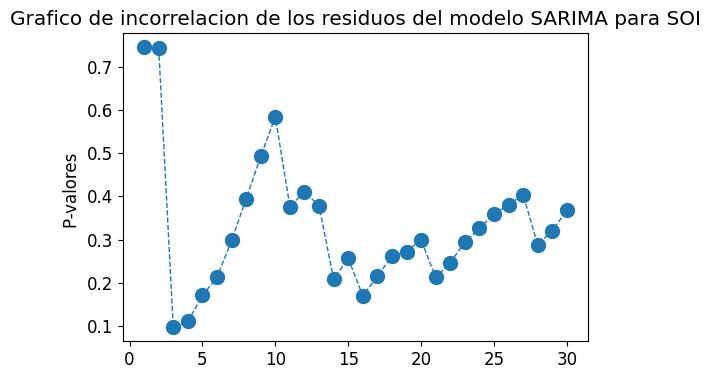
\includegraphics[scale=.52]{Figures/inco_soi.png}
\caption{SOI: gráfico de incorrelación (p--valores Ljung--Box por lag).}
\label{fig:inco_soi}
\end{figure}



\begin{figure}[H]\centering
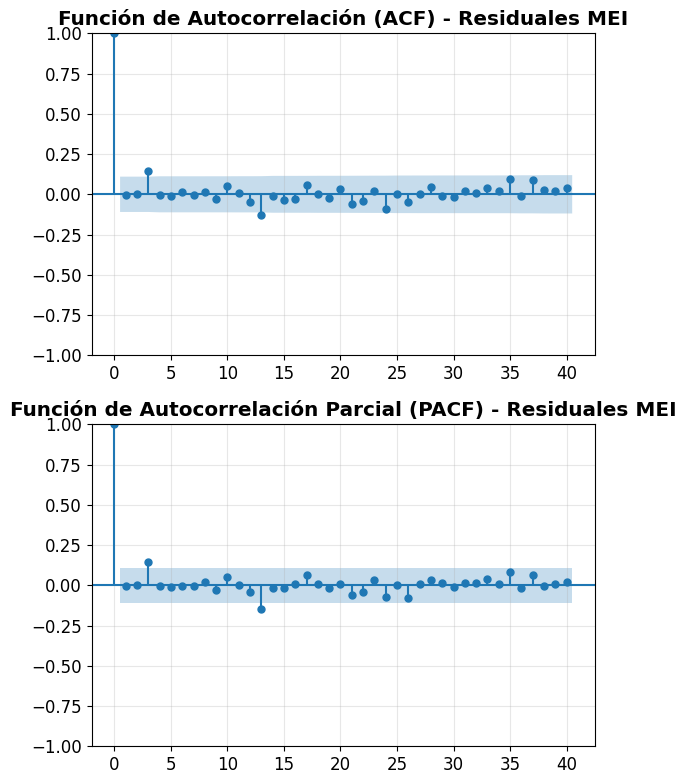
\includegraphics[scale=.52]{Figures/acf_pacf_res_mei.png}
\caption{MEI: ACF y PACF de los residuos.}
\label{fig:acf_pacf_res_mei}
\end{figure}

\begin{figure}[H]\centering
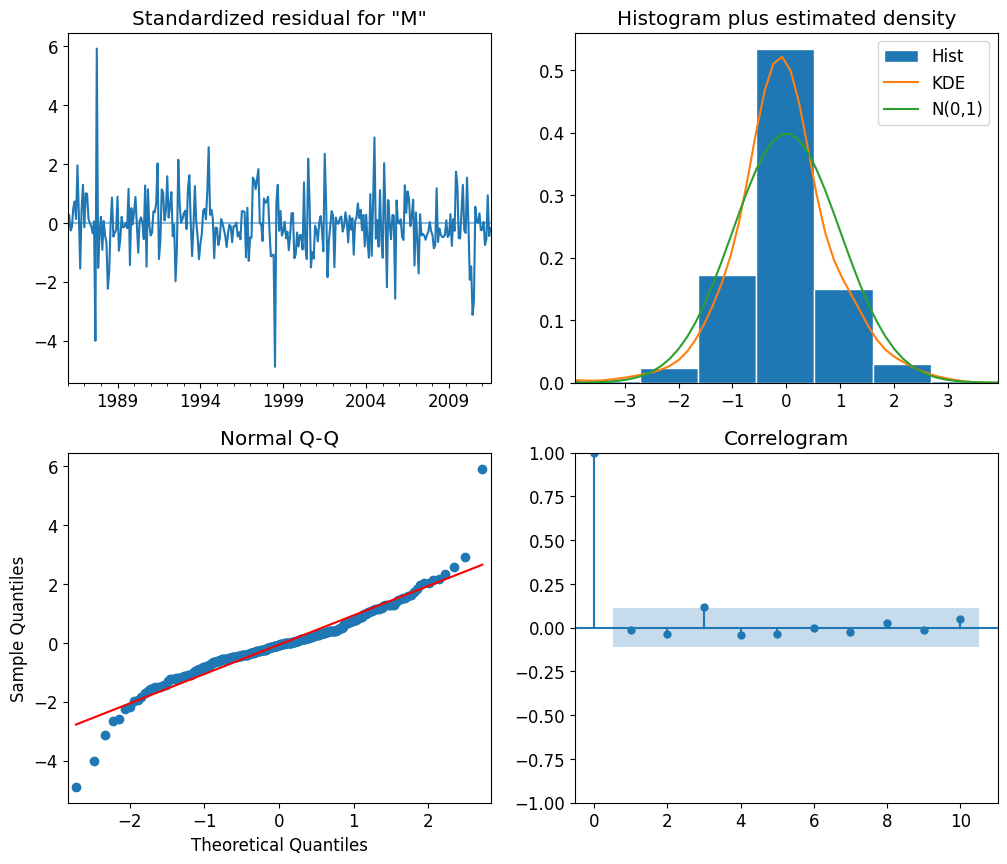
\includegraphics[scale=.52]{Figures/res_std_mei.png}
\caption{MEI: diagnóstico estándar de residuos (histograma, densidad, Q--Q, correlograma).}
\label{fig:std_mei}
\end{figure}

\begin{figure}[H]\centering
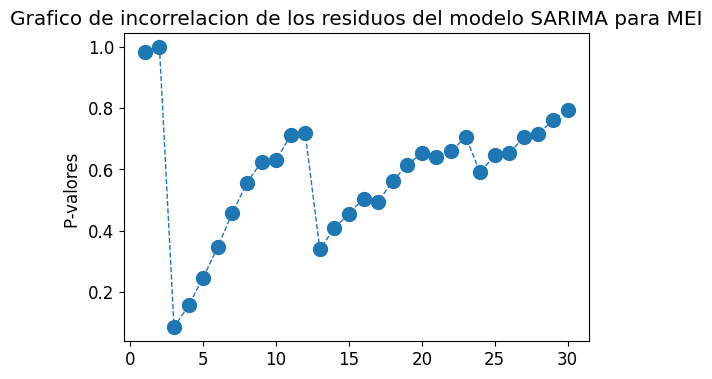
\includegraphics[scale=.52]{Figures/inco_mei.png}
\caption{MEI: gráfico de incorrelación (p--valores Ljung--Box por lag).}
\label{fig:inco_mei}
\end{figure}

\begin{figure}[H]\centering
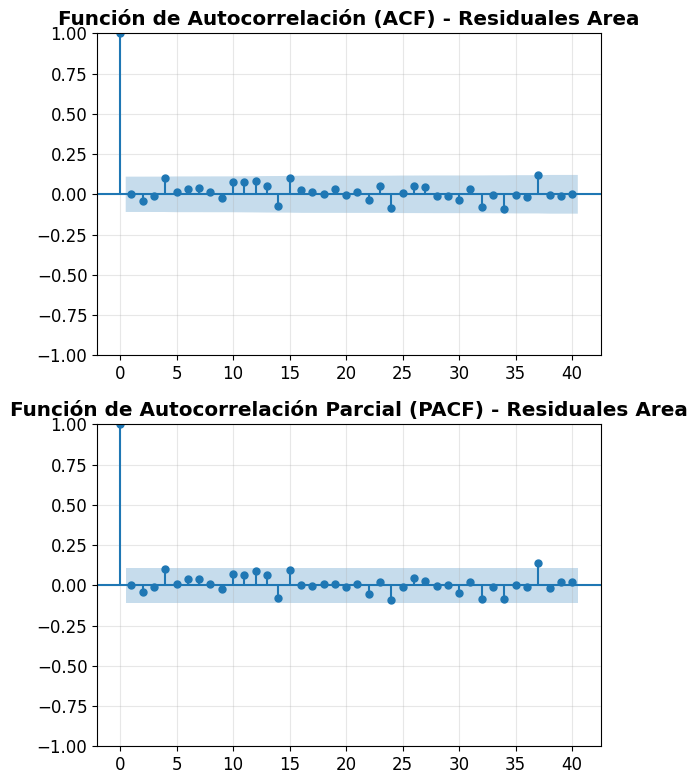
\includegraphics[scale=.52]{Figures/acf_pacf_res_area.png}
\caption{Área: ACF y PACF de los residuos.}
\label{fig:acf_pacf_res_area}
\end{figure}

\begin{figure}[H]\centering
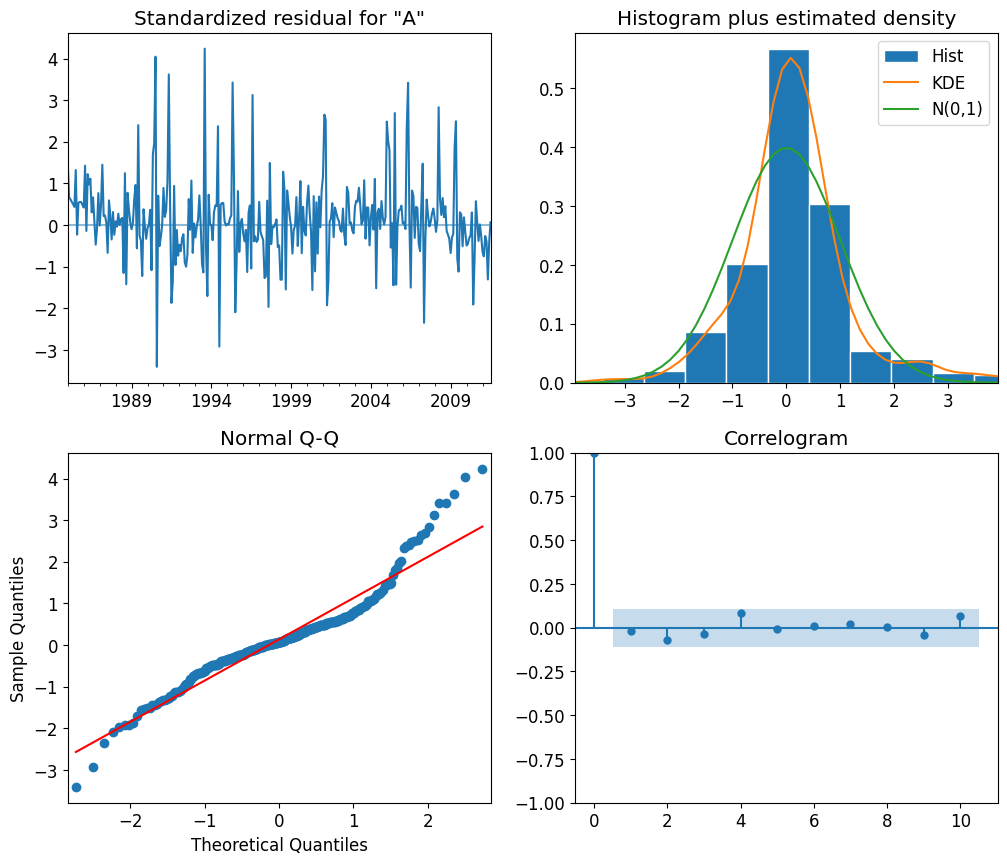
\includegraphics[scale=.52]{Figures/res_std_area.png}
\caption{Área: diagnóstico estándar de residuos (histograma, densidad, Q--Q, correlograma).}
\label{fig:std_area}
\end{figure}

\begin{figure}[H]\centering
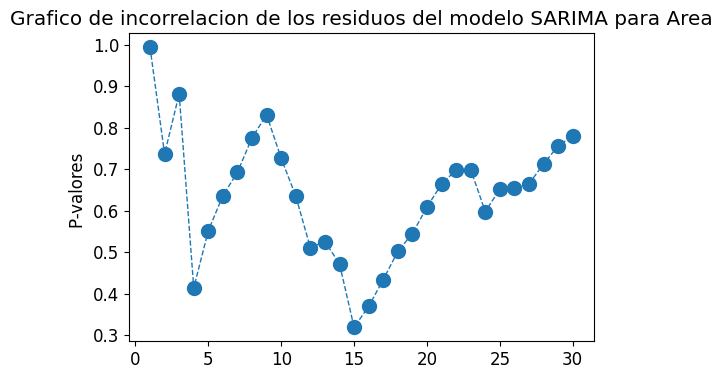
\includegraphics[scale=.52]{Figures/inco_area.png}
\caption{Área: gráfico de incorrelación (p--valores Ljung--Box por lag).}
\label{fig:inco_area}
\end{figure}

\begin{figure}[H]
    \centering
    \includegraphics[scale=.42]{Figures/facp_Area_dif.png}
    \caption{Funciones ACF y PACF de la serie Área (superficie de agua).}
    \label{fig:facp_area_dif}
\end{figure}

\begin{figure}[H]\centering
\includegraphics[scale=.52]{Figures/acf_pacf_res_area_d.png}
\caption{Área (diferenciada): ACF y PACF de los residuos.}
\label{fig:acf_pacf_res_area_d}
\end{figure}

\begin{figure}[H]\centering
\includegraphics[scale=.52]{Figures/res_std_area_d.png}
\caption{Área (diferenciada): diagnóstico estándar de residuos (histograma, densidad, Q--Q, correlograma).}
\label{fig:std_area_d}
\end{figure}

\begin{figure}[H]\centering
\includegraphics[scale=.52]{Figures/inco_area_d.png}
\caption{Área (diferenciada): gráfico de incorrelación (p--valores Ljung--Box por lag).}
\label{fig:inco_area_d}
\end{figure}

\begin{figure}[H]\centering
\includegraphics[scale=.30]{Figures/res_sarima_oni.png}
\caption{ONI: residuos del modelo SARIMA.}
\label{fig:res_oni}
\end{figure}

\begin{figure}[H]\centering
\includegraphics[scale=.42]{Figures/pred_oni.png}
\caption{ONI: observado (train+test) vs. predicciones con IC 95\%.}
\label{fig:pred_oni}
\end{figure}



\begin{figure}[H]\centering
\includegraphics[scale=.30]{Figures/res_sarima_soi.png}
\caption{SOI: residuos del modelo SARIMA.}
\label{fig:res_soi}
\end{figure}


\begin{figure}[H]\centering
\includegraphics[scale=.42]{Figures/pred_soi.png}
\caption{SOI: observado (train+test) vs. predicciones con IC 95\%.}
\label{fig:pred_soi}
\end{figure}

\begin{figure}[H]\centering
\includegraphics[scale=.30]{Figures/res_sarima_mei.png}
\caption{MEI: residuos del modelo SARIMA.}
\label{fig:res_mei}
\end{figure}


\begin{figure}[H]\centering
\includegraphics[scale=.42]{Figures/pred_mei.png}
\caption{MEI: observado (train+test) vs. predicciones con IC 95\%.}
\label{fig:pred_mei}
\end{figure}

\begin{figure}[H]\centering
\includegraphics[scale=.30]{Figures/res_sarima_area.png}
\caption{Área: residuos del modelo SARIMA.}
\label{fig:res_area}
\end{figure}

\begin{figure}[H]\centering
\includegraphics[scale=.42]{Figures/pred_area.png}
\caption{Área: observado (train+test) vs. predicciones con IC 95\%.}
\label{fig:pred_area}
\end{figure}


\begin{figure}[H]\centering
\includegraphics[scale=.30]{Figures/res_sarima_area_d.png}
\caption{Área (diferenciada): residuos del modelo SARIMA.}
\label{fig:res_area_d}
\end{figure}


\begin{figure}[H]\centering
\includegraphics[scale=.42]{Figures/pred_area_d.png}
\caption{Área (diferenciada): observado (train+test) vs. predicciones con IC 95\%.}
\label{fig:pred_area_d}
\end{figure}

\begin{figure}[H]
    \centering
    \includegraphics[scale=0.32]{Figures/var_pred.png}
    \caption{Predicciones del modelo VAR(3) frente a los valores reales de ONI, SOI, MEI y Área.}
    \label{fig:var_pred}
\end{figure}

%----------------------------------------------------------------------------------------
% Bibliografía
%----------------------------------------------------------------------------------------

\renewcommand{\bibname}{Bibliografía} % Para asegurarte de que el título sea correcto
\phantomsection % Necesario para que el enlace del marcador sea correcto

\printbibliography[heading=bibintoc]

\end{document}






